\documentclass[pdftex, a4paper, 10pt]{book}

\usepackage{amsmath}
\usepackage{graphicx}
\usepackage{hyperref}
\usepackage{listings}
\usepackage{makeidx}
\usepackage{plain}

\lstset{language=C++, basicstyle=\footnotesize, showstringspaces=false}

\newtheorem{definition}{Definition}
\newtheorem{theorem}{Theorem}
\newtheorem{example}{Example}
\newtheorem{problem}{Problem}

%\makeindex

\begin{document}

\vspace{5cm}

\begin{figure}[h!]
\begin{center}

\includegraphics[width=1.0\textwidth]{opennn_logo_name}
\end{center}
\href{http://www.intelnics.com/opennn}{http://www.intelnics.com/opennn}\newline

Version 1.0 manual\newline

January 2014.
\end{figure}

\begin{center}
\end{center}

\vspace{5cm}

{
\Large
\textbf{}\newline
\textbf{Roberto Lopez}\newline
Intelnics - \textit{The artificial intelligence company}\newline 
\href{mailto:robertolopez@intelnics.com}{\nolinkurl{robertolopez@intelnics.com}}
}

\vspace{5cm}


\begin{verbatim}
Copyright (c) 2014 Roberto Lopez.
Permission is granted to copy, distribute and/or modify this document
under the terms of the GNU Free Documentation License, Version 1.3
or any later version published by the Free Software Foundation;
A copy of the license is included in the OpenNN folder called "license". 
\end{verbatim}
      
\chapter*{Preface}	
Neural networks have found a wide range of applications,
which include function regression, pattern recognition, time series
prediction, optimal control, optimal shape
design or inverse problems. A neural network can learn either from data sets or from mathematical models. 

\texttt{OpenNN} is a comprehensive class library which implements neural networks
 in the C++ programming language. 
This software tool can be used
for the whole range of applications mentioned above. \texttt{OpenNN}
also provides a workaround for the solution of function optimization
problems. The library has been released as the open source GNU
Lesser General Public License.

This manual is organized as follows: 
Chapter \ref{Preliminaries} provides some guidelines for installing the software and using some basic data structures, 
such as vectors and matrices. 
In Chapter \ref{NeuralNetworksBasis}, a brief introduction to the principal concepts of neural networks is given. 
Also, in Chapter \ref{SoftwareModelBasis} the most general software model of \texttt{OpenNN} is presented.
Chapters \ref{NeuralNetwork}, \ref{PerformanceFunctional} and \ref{TrainingStrategy} state the learning problem for neural networks and provide a collection of related algorithms. 
In Chapters \ref{FunctionRegression}, \ref{PatternRecognition}, \ref{OptimalControl}, \ref{OptimalShapeDesign} and \ref{InverseProblems} the most important learning tasks for neural networks are formulated and several practical applications are also presented. 
Finally, Chapter \ref{FunctionOptimization} explains how to solve function optimization problems by means of \texttt{OpenNN}.

%Appendixes \ref{SoftwareModel} and \ref{UnitTesting} present some activities related to the software engineering process of \texttt{OpenNN}. 
%Finally, Appendix \ref{NumericalIntegration} introduces some numerical integration algorithms. 
	
 
\tableofcontents

%%%%%%%%%%%%%%%%%%%%%%%%%%%%%%%%%%%%%%%%%%%%%%%%%%%%%%%%%%%%%%%%%%%%%%%%%%%%%%%%%%%%

\chapter{Preliminaries}\label{Preliminaries}

\section{Building OpenNN}\label{BuildingOpenNN}
\texttt{OpenNN} has been written in ANSI C++. 
This means that the library can be built on any operating system with little effort. 
In this regard, project files of Qt Creator are included.
Nevertheless, \texttt{OpenNN} does not make use of the Qt Library. 
When working with another compiler is needed, a project for it must be created.

\subsection*{Compiling OpenNN}

Compiling \texttt{OpenNN} is easy, since it comes with project files for the latest version of Qt creator.
Qt Creator is a cross-platform IDE (integrated development environment), which is part of the Qt Project.
It can be downloaded from the following site:

\begin{flushleft}
\href{http://qt-project.org/downloads}{http://qt-project.org/downloads}
\end{flushleft}

Note that, although \texttt{OpenNN} comes with project files for Qt Creator, it does not make use of the Qt Library.
The \lstinline"opennn.pro" project file can be found in the \lstinline"opennn" folder.
To open the \texttt{OpenNN} project just double click on that file. 
A similar window than that depicted in Figure \ref{QtCreatorProject} should come up.

\begin{figure}[h!]
\begin{center}
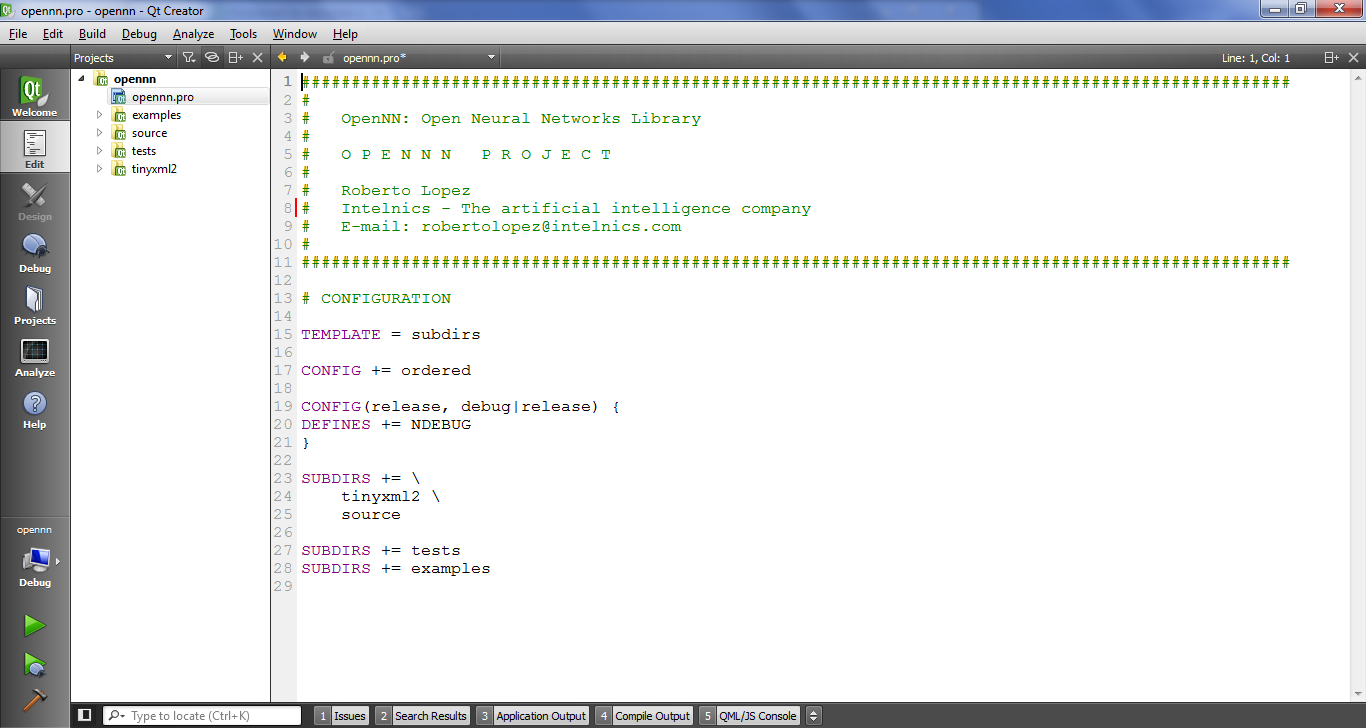
\includegraphics[width=1.0\textwidth]{preliminaries/qt_creator_project}
\caption{Qt Creator project view.}\label{QtCreatorProject}
\end{center}
\end{figure}


\subsubsection*{2. Running the test suite.}

From the \lstinline"opennn" project, select the \lstinline"test" subproject. 
That can be found at the bottom left of Qt Creator.   
Clicking on the play button or pressing \lstinline"Ctrl+R" will compile, build and run the test suite application. 
The terminal will show the following message:

\begin{lstlisting}
...

OpenNN test suite results:
Tests run: tests_run
Tests passed: tests_run
Tests failed: 0
Test OK
\end{lstlisting}

This guarantees that \texttt{OpenNN} has been compiled properly, together with all the libraries included.

\subsubsection*{3. Running an example.}

Many example subprojects are also included in the \texttt{OpenNN} distribution.
From the \lstinline"opennn" project select some example, for instance the \lstinline"simple_function_regression" subproject.  
Then run that example by clicking on the play button or pressing \lstinline"Ctrl+R".
Read the application code to see what the simple function regression example does. 


\section{OpenNN namespace}\label{OpenNNNamespace}
\index{namespace}
\index{OpenNN namespace}

Each set of definitions in the \texttt{OpenNN} library is `wrapped'
in the namespace \lstinline"OpenNN". In this way, if some other
definition has an identical name, but is in a different namespace,
then there is no conflict.

The \lstinline"using" directive makes a namespace available
throughout the file where it is written \cite{Eckel2000}. For the
\lstinline"OpenNN" namespace the following sentence can be written:

\begin{lstlisting}
using namespace OpenNN;
\end{lstlisting}



\section{Vector template}\label{VectorTemplate}
\index{Vector class}

The \lstinline"Vector" class is a template, which means that it
can be applied to different types \cite{Eckel2000}. That is, we
can create a \lstinline"Vector" or \lstinline"int" numbers, \lstinline"MyClass" objects, etc.

The \lstinline"Vector" in \texttt{OpenNN} is derived from the \lstinline"vector" in the Standard Template Library. 

\subsubsection*{Members}

The onl member of the \lstinline"Vector" class is:

\begin{itemize}
\item[-] A double pointer to some type. 
\end{itemize}

That two class members are declared as being private. 

\subsubsection*{File format}

Vector objects can be serialized or deserialized to or from a data file which contains the member values. The file format is as follows.

\begin{lstlisting}
element_0 element_1 ... element_N
\end{lstlisting}

\subsubsection*{Constructors}

Multiple constructors are defined in the \lstinline"Vector" class, where the different constructors take different parameters. 

% Default constructor

The easiest way of creating a vector object is by means of the default constructor, wich builds a vector of size zero.
For example, in order to construct an empty \lstinline"Vector" of
\lstinline"int" numbers we use

\begin{lstlisting}
Vector<int> v;
\end{lstlisting}

% Size constructor

The following sentence constructs a \lstinline"Vector" of $3$
\lstinline"double" numbers.

\begin{lstlisting}
Vector<double> v(3);
\end{lstlisting}

% Size initialization constructor

If we want to construct \lstinline"Vector" of $5$ \lstinline"bool"
variables and initialize all the elements to $false$, we can use

\begin{lstlisting}
Vector<bool> v(5, false);
\end{lstlisting}

% File constructor

It is also possible to construct an object of the \lstinline"Vector" class and at the same time 
load its members from a file. In order to do that we can do

\begin{lstlisting}
Vector<int> v(`Vector.dat');
\end{lstlisting}

The file `Vector.dat' contains a first row with the size of the vector and an aditional row for each element of the vector. 

% Copy constructor

The following sentence constructs a \lstinline"Vector" which is a copy of another \lstinline"Vector",

\begin{lstlisting}
Vector<MyClass> v(3);
Vector<MyClass> w(v);
\end{lstlisting}

\subsubsection*{Operators}

The \lstinline"Vector" class also implements different types of operators for assignment, reference, arithmetics or comparison. 

% Assignment operator 

The assignment operator copies a vector into another vector, 

\begin{lstlisting}
Vector<int> v;
Vector<int> w = v;
\end{lstlisting}

% Reference operator 

The following sentence constructs a vector and sets the values of their elements using the reference operator. Note
that indexing goes from $0$ to $n-1$, where $n$ is the
\lstinline"Vector" size.

\begin{lstlisting}
Vector<double> v(3);
v[0] = 1.0;
v[1] = 2.0;
v[2] = 3.0;
\end{lstlisting}

% Arithmetic operators 

Sum, difference, product and quotient operators are included in the \lstinline"Vector" class to perform arithmetic operations with a scalar or another \lstinline"Vector". Note that the arithmetic operators with another \lstinline"Vector" require that they have the same sizes. 

The following sentence uses the vector-scalar sum operator, 

\begin{lstlisting}
Vector<int> v(3, 1.0);
Vector<int> w = v + 3.1415926;
\end{lstlisting}

An example of the use of the vector-vector multiplication operator is given below, 

\begin{lstlisting}
Vector<double> v(3, 1.2);
Vector<double> w(3, 3.4);
Vector<double> x = v*w;
\end{lstlisting}

% Arithmetic and assignment operators

Assignment by sum, difference, product or quotient with a scalar or another \lstinline"Vector" is also possible by using the arithmetic and assignent operators. If another \lstinline"Vector" is to be used, it must have the same size.

For instance, to assign by difference with a scalar, we migh do

\begin{lstlisting}
Vector<int> v(3, 2);
v -= 1;
\end{lstlisting}
 
In order to assign by quotation with another \lstinline"Vector", we can write 

\begin{lstlisting}
Vector<double> v(3, 2.0);
Vector<double> w(3, 0.5);
v /= w;
\end{lstlisting}

% Equality and relational operators

Equality and relational operators are also implemented here. They can be used with a scalar or another \lstinline"Vector". For the last case the same sizes are assumed. 

An example of the equal to operator with a scalar is 

\begin{lstlisting}
Vector<bool> v(5, false);
bool is_equal = (v == false);
\end{lstlisting}

The less than operator with another \lstinline"Vector" can be used as follows,

\begin{lstlisting}
Vector<int> v(5, 2.3);
Vector<int> w(5, 3.2);
bool is_less = (v < w);
\end{lstlisting}

\subsubsection*{Methods}

Get and set methods for each member of this class are implemented to exchange information among objects. 

% Size and element methods

The method \lstinline"size" returns the size of a \lstinline"Vector".

\begin{lstlisting}
Vector<MyClass> v(3);
int size = v.size();
\end{lstlisting}

On the other hand, the method \lstinline"set" sets a new size to a \lstinline"Vector". 
Note that the element values of that \lstinline"Vector" are lost. 

\begin{lstlisting}
Vector<bool> v(3);
v.set(6);
\end{lstlisting}

% Initialization methods

If we want to initialize a vector at random we can use the \lstinline"initialize_uniform" or \lstinline"initialize_normal" methods, 

\begin{lstlisting}
Vector<double> v(5);
v.initialize_uniform();
Vector<double> w(3);
w.initialize_normal();
\end{lstlisting}

% Mathematical methods

The \lstinline"Vector" class also includes some mathematical methods which can be useful in the development of neural networks algorithms and applications. 

The \lstinline"calculate_norm" method calculates the norm of the vector, 

\begin{lstlisting}
Vector<double> v(5, 3.1415927);
double norm = v.calculate_norm();
\end{lstlisting}

In order to calculate the dot product between this \lstinline"Vector" and another \lstinline"Vector" we can do

\begin{lstlisting}
Vector<double> v(3, 2.0);
Vector<double> w(3, 5.0);
double dot = v.dot(w);
\end{lstlisting}

We can calculate the mean or the standard deviation values of the elements in a \lstinline"Vector" by using the \lstinline"calculate_mean" and \lstinline"calculate_standard_deviation" methods, respectively. For instance

\begin{lstlisting}
Vector<double> v(3, 4.0);
double mean = v.calculate_mean();
double standard_deviation = v.calculate_standard_deviation();
\end{lstlisting}

% Utility methods

Finally, utility methods for serialization or loading and saving the class members to a file are also included. 
In order to obtain a \lstinline"std::string" representation of a \lstinline"Vector" object we can make
 
\begin{lstlisting}
Vector<bool> v(1, false);
std::string vector_string = v.to_string();
\end{lstlisting}

To save a \lstinline"Vector" object to a file we can do

\begin{lstlisting}
Vector<int> v(2, 0);
v.save(`Vector.dat');
\end{lstlisting}

The first row of the file \lstinline"Vector.dat" is the size of the vector and the other rows contain the values of the elements of that vector. 

If we want to load a \lstinline"Vector" object from a data file we could write

\begin{lstlisting}
Vector<double> v;
v.load(`Vector.dat');
\end{lstlisting}

Where the format of the \lstinline"Vector.dat" file must be the same as that described above. 




\section{Matrix template}\label{MatrixTemplate}
\index{Matrix class}

As it happens with the \lstinline"Vector" class, the \lstinline"Matrix" class is also a template \cite{Eckel2000}. 
Therefore, a \lstinline"Matrix" of any type can be created. 

\subsubsection*{Members}

The \lstinline"Matrix" class has three members:

\begin{itemize}
\item[-] The number of rows. 
\item[-] The number of columns. 
\item[-] A double pointer to some type. 
\end{itemize}

That members are private. Private members can be accessed only within methods of the class itself.

\subsubsection*{File format}

The member values of a matrix object can be serialized or deserialized to or from a data file. 
The format is as follows. 

\begin{lstlisting}
element_00 ... element_0M
...
element_N0 ... element_NM
\end{lstlisting}

\subsubsection*{Constructors}

The \lstinline"Matrix" class also implements multiple constructors, with different parameters.

% Default constructor

The default constructor creates a matrix with zero rows and zero columns, 

\begin{lstlisting}
Matrix<MyClass> m;
\end{lstlisting}

% Rows and columns numbers constructor

In order to construct an empty \lstinline"Matrix" with a specified number of rows and columns we use

\begin{lstlisting}
Matrix<int> m(2, 3);
\end{lstlisting}

% Initialization constructor

We can specify the number of rows and columns and initialize the \lstinline"Matrix" elements at the same time by doing

\begin{lstlisting}
Matrix<double> m(1, 5, 0.0);
\end{lstlisting}

% File constructor

To build a \lstinline"Matrix" object by loading its members from a data file the following constructor is used, 

\begin{lstlisting}
Matrix<double> m(`Matrix.dat');
\end{lstlisting}

The format of a matrix data file is as follows: the first line contains the numbers of rows and columns separated by a blank space; the following data contains the matrix elements arranged in rows and columns. For instance, the next data will correspond to a \lstinline"Matrix" of zeros with 2 rows and 3 columns,

\begin{lstlisting}
2 3
0 0 0
0 0 0
\end{lstlisting}

% Copy constructor

The copy constructor builds an object which is a copy of another object, 

\begin{lstlisting}
Matrix<bool> a(3,5);
Matrix<bool> b(a);
\end{lstlisting}

\subsubsection*{Operators}

% Assignment operator 

The \lstinline"Matrix" class also implements the assignment operator, 


\begin{lstlisting}
Matrix<double> a(2,1);
Matrix<bool> b = a;
\end{lstlisting}

% Reference operator 

Below there is an usage example of the reference operator here. Note that row indexing goes from \lstinline"0" to
\lstinline"rows_number-1"  and column indexing goes from \lstinline"0" to \lstinline"columns_number-1".

% Arithmetic operators 

\begin{lstlisting}
Matrix<int> m(2, 2);
m[0][0] = 1;
m[0][1] = 2;
m[1][0] = 3;
m[1][1] = 4;
\end{lstlisting}

% Arithmetic operators

The use of the arithmetic operators for the \lstinline"Matrix" class are very similar to those for the \lstinline"Vector" class. The following sentence uses the scalar difference operator, 

\begin{lstlisting}
Matrix<double> a(5, 7, 2.5);
Matrix<double> b = a + 0.1;
\end{lstlisting}

% Arithmetic and assignment operators

Also, using the arithmetic and assignment operators with the \lstinline"Matrix" class is similar than with the \lstinline"Vector" class. For instance, to assign by sum with another \lstinline"Matrix" we can write

\begin{lstlisting}
Matrix<double> a(1, 2, 1.0);
Matrix<double> b(1, 2, 0.5);
a += b;
\end{lstlisting}

% Equality and relational operators

The not equal to operator with another \lstinline"Matrix" can be used in the following way, 

\begin{lstlisting}
Matrix<std::string> a(1, 1, `hello');
Matrix<std::string> b(1, 1, `good bye');
bool is_not_equal_to = (a != b);
\end{lstlisting}

The use of the greater than operator with a scalar is listed below

\begin{lstlisting}
Matrix<double> a(2, 3, 0.0);
bool is_greater_than = (a > 1.0);
\end{lstlisting}

\subsubsection*{Methods}

As it happens for the \lstinline"Vector" class, the \lstinline"Matrix" class implements get and set methods for all the members. 

The \lstinline"get_rows_number" and \lstinline"get_columns_number" methods are very useful, 

\begin{lstlisting}
Matrix<MyClass> m(4, 2);
int rows_number = m.get_rows_number();
int columns_number = m.get_columns_number();
\end{lstlisting}

In order to set a new number of rows or columns to a \lstinline"Matrix" object, the \lstinline"set_rows_number" or \lstinline"set_columns_number" methods are used,

\begin{lstlisting}
Matrix<bool> m(1, 1);
m.set_rows_number(2);
m.set_columns_number(3);
\end{lstlisting}

% Initialization methods

A \lstinline"Matrix" can be initialized with a given value, at random with an uniform distribution or at random with a normal distribution, 

\begin{lstlisting}
Matrix<double> m(4, 2);
m.initialize(0.0);
m.initialize_uniform(-0.2, 0.4);
m.initialize_normal(-1.0, 0.25);
\end{lstlisting}

% Mathematical methods

A set of mathematical methods are also implemented for convenience. For instance, the \lstinline"dot" method computes the dot product of this \lstinline"Matrix" with a \lstinline"Vector" or with another \lstinline"Matrix",

\begin{lstlisting}
Matrix<double> m(4, 2, 1.0);
Vector<double> v(4, 2.0);
Vector<double> dot_product = m.dot(v);
\end{lstlisting}

% Utility methods

Finally, string serializing, printing, saving or loading utility methods are also implemented. For example, the use of the \lstinline"print" method is

\begin{lstlisting}
Matrix<bool> m(1, 3, false);
m.print();
\end{lstlisting}


%%%%%%%%%%%%%%%%%%%%%%%%%%%%%%%%%%%%%%%%%%%%%%%%%%%%%%%%%%%%%%%%%%%%%%%%%%%%%%%%%%%%

\chapter{Neural networks basis}\label{NeuralNetworksBasis}
\index{neural networks}

In this Chapter we formulate the learning problem for neural networks and describe some learning tasks that they can solve. 


\section{Learning problem}\label{LearningProblem}
\index{neuron model}
\index{perceptron}

\index{network architecture}
\index{feed-forward architecture}

\index{objective functional}
\index{performance functional|see{objective functional}}

\index{training algorithm}
\index{learning algorithm|see{training algorithm}}

Any application for neural networks involves a neural network itself, a performance functional, and a training strategy. 
The learning problem is then formulated as to find a neural network which optimizes a performance functional by means of a training strategy.

\subsubsection*{Neural network}

A neuron model is a mathematical model of the behavior of a single neuron in a
biological nervous system. 
The most important neuron model is the so called perceptron. 
The perceptron neuron model receives information in the form of numerical inputs. 
This information is then combined with a set of parameters to produce a message in the form of a
single numerical output.

Most neural networks, even biological neural networks, exhibit a layered struc-
ture. In this work layers are the basis to determine the architecture of a
neural network. A layer of perceptrons taks a set of inputs in order to produce a set of outptus. 

A multilayer perceptron is
built up by organizing layers of perceptrons in a network architecture.
In this way, the architecture of a network refers to the number of
layers, their arrangement and connectivity. The characteristic
network architecture in \texttt{OpenNN} is the so called
feed-forward architecture. 
The multilayer perceptron can then be defined as a network architecture of perceptron layers. 
This neural network represents a parameterized function of several variables with very good approximation properties. 

In order to solve practical applications, different extensions must be added to the multilayer perceptron. 
Some of them include scaling, unscaling, bounding, probabilistic or conditions layers.
Therefore, the neural network in \texttt{OpenNN} is composed by a mutlilayer perceptron plus some additional layers. 

\subsubsection*{Performance functional}

The performance functional plays an important role in the use of a neural
network. It defines the task the neural network is required to do
and provides a measure of the quality of the representation that the
neural network is required to learn. The choice of a suitable performance
functional depends on the particular application.

A performance functional in \texttt{OpenNN} is composed of three different terms: objective, regularization and constraints. 
Most of the times, a single objective term will be enough, but some applications will require regularize solutions 
or will be defined by constraints on the solutions. 

Learning tasks such as function regression and pattern recognition will have performance functionals measured on data sets. 
On the other hand, learning tasks such ase optimal control or optimal shape design will have performance functionasl measured on mathematical models.
Finally, the performance functionals in another learning tasks, such ase inverse problems, will be measured in both data sets and mathematical models.  

\subsubsection*{Training strategy}

The procedure
used to carry out the learning process is called training (or learning) strategy.
The training strategy is applied to the neural 
network to in order to obtain the best possible performance. The type of
training is determined by the way in which the adjustment of the
parameters in the neural network takes place.

The most general training strategy in \texttt{OpenNN} will include three different training algorithms: initialization, main and refinement. 
Most applications will only need one training algorithm, but some complex problems might require the combination of two or three of them. 

A generally good training strategy includes the quasi-Newton method. 
However, noisy problems might require an evolutionary algorithm. 
The first cited training algorithm is several orders of magnitude faster than the second one. 

\subsubsection*{Learning activity diagram}

The learning problem for neural networks is formulated from a
variational point of view. Indeed, learning tasks lie in terms
of finding a function which causes some functional to assume an
extreme value. Neural networks provide a
general framework for solving variational problems.

Figure \ref{LearningActivityDiagram} depicts an activity diagram for the learning problem. 
The solving approach
here consists of three steps. The first step is to choose a suitable
neural network which will approximate the solution to the problem. 
In the second step the
variational problem is formulated by selecting an appropriate
performance functional.
The third step is to solve the reduced function optimization
problem with a training strategy capable of
finding an optimal set of parameters.

\begin{figure}[h!]
\begin{center}
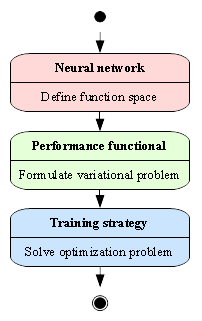
\includegraphics[width=0.35\textwidth]{neural_networks_basis/learning_problem}
\caption{Learning problem for neural networks.}\label{LearningActivityDiagram}
\end{center}
\end{figure}


\section{Learning tasks}\label{LearningTasks}
\index{function regression}
\index{pattern recognition}
\index{optimal control}
\index{inverse problems}
\index{optimal shape design}
\index{function optimization}

Learning tasks for neural networks can be classified according to the source of information for them. 
There are basically two sources of information: data sets and mathematical models. 
In this way, some classes of learning tasks which learn from data sets are function regression, pattern recognition or time series prediction. 
On the other hand, learning tasks in which learning is performed from mathematical models are optimal control or optimal shape design. 
Finally, in inverse problems the neural network learns from both data sets and mathematical models.

\subsubsection*{Function regression}

Function regression is the most popular learning task for neural networks. 
It is also called modelling. The function regression problem can be regarded as the problem of
approximating a function from a data set consisting of input-target instances
\cite{Haykin1994}. The targets are a specification
of what the response to the inputs should be \cite{Bishop1995}. 
While input variables might be quantitative or qualitative, in function regression target variables are quantitative. 

Performance measures for function regression are based on a sum of errors between the outputs from the neural network and the targets in the training data. 
As the training data is usually defficient, a regularization term might be required in order to solve the problem correctly.  

An example is to design an instrument that can determine serum cholesterol levels from
measurements of spectral content of a blood sample. There are a number of 
patients for which there are measurements of several wavelengths of the spectrum.
For the same patients there are also measurements of several
cholesterol levels, based on serum separation \cite{Demuth2009}. 

\subsubsection*{Pattern recognition}

The learning task of pattern recognition gives raise to artificial intelligence. That problem can be stated as
the process whereby a received pattern, characterized by a distinct
set of features, is assigned to one of a prescribed number of
classes \cite{Haykin1994}. Pattern recognition is also known as classification. Here
the neural network learns from knowledge represented by a training
data set consisting of input-target instances. The inputs include a
set of features which characterize a pattern, and they can be quantitative or qualitative. The targets specify
the class that each pattern belongs to and therefore are qualitative \cite{Bishop1995}.

Classification problems can be, in fact, formulated as being modelling problems. 
As a consequence, performance functionals used here are also based on the sum squared error. 
Anyway, the learning task of pattern recognition is more difficult to solve than that of function regression. 
This means that a good knowledge of the state of the technique is recommended for success. 

A typical example is to disinguish hand-written versions of characters. 
Images of the characters might be captured and fed to a computer. 
An algorithm is then seek to which can distinguish as reliably as possible between the characters \cite{Bishop1995}. 

\subsubsection*{Optimal control}

Optimal control is playing an increasingly important role in the
design of modern engineering systems. The aim
here is the optimization, in some defined sense, of a physical
process. More specifically, the objective of these problems is to
determine the control signals that will cause a process to satisfy
the physical constraints and at the same time minimize or maximize
some performance criterion \cite{Kirk1970} \cite{BalsaCanto2001}. 

The knowledge in optimal control problems is not represented in the form of a data set, it is given by a mathematical model. 
These objective functionals are often defined by integrals, ordinary differential equations or partial differential equations. 
In this way, and in order to evaluate them, we might need to apply Simpon methods, Runge-Kutta methods or finite element methods. 
Optimal control problems often include constraints. 

As a simple example, consider the problem of a rocket launching a
satellite into an orbit around the earth. An associated optimal
control problem is to choose the controls (the thrust attitude angle
and the rate of emission of the exhaust gases) so that the rocket
takes the satellite into its prescribed orbit with minimum
expenditure of fuel or in minimum time.

\subsubsection*{Optimal shape design}

Optimal shape design is a very interesting field for industrial
applications. The goal in these problems
is to computerize the development process of some tool, and
therefore shorten the time it takes to create or to improve the
existing one. Being more precise, in an optimal shape design process
one wishes to optimize some performance criterium involving the
solution of a mathematical model with respect to its domain of
definition \cite{Bucur2005}. 

As in the previous case, the neural network here learns from a mathematical model. 
Evaluation of the performance functional here might also need the integration of functions, ordinary differential equations or partial differential equations. 
Optimal shape design problems defined by partial differential equations are challenging applications. 

One example is the design of airfoils,
which proceeds from a knowledge of computational fluid dynamics
\cite{Eyi1994} \cite{Mohammadi2004}. The performance goal here might
vary, but increasing lift and reducing drag are among the most common. Other objectives as weight reduction, stress reinforcement and
even noise reduction can be obtained. On the other hand, the airfoil
may be required to achieve this performance with constraints on
thickness, pitching moment, etc.

\subsubsection*{Inverse problems}

Inverse problems can be described as being opposed to direct
problems. In a direct problem the cause is given, and the effect is
determined. In an inverse problem the effect is given, and the cause
is estimated \cite{Kirsch1996} \cite{Sabatier2000} \cite{Ramm2005}.
There are two main types of inverse problems: input estimation, in
which the system properties and output are known and the input is to
be estimated; and properties estimation, in which the the system
input and output are known and the properties are to be estimated.
Inverse problems can be found in many areas of science and
engineering. 

This type of problems is of great interest from both a theoretical and practical perspectives. 
From a theoretical point of view, the neural network here needs both mathematical models and data sets. 
The aim is usually formulated as to find properties or inputs which make a mathematical model to comply with the data set. 
From a practical point of view, most numerical software must be tuned up before being on production. 
That means that the particular properties of a system must be properly estimated in order to simulate it well.

A typical inverse problem in geophysics is to find the 
subsurface inhomogeneities from collected scattered fields caused by
acoustic waves sent at the surface and a mathematical model of soil mechanics.  

\subsubsection*{Tasks companion diagram}

As we have said, the knowledge for a neural network can be represented in the form of data sets or mathematical models. 
The neural network learns from data sets in function regression and pattern recognition; 
it learns from mathematical models in optimal control and optimal shape design; 
and it learns from both mathematical models and data sets in inverse problems. 
Please note that other possible applications can be added to these learning tasks. 

Figure \ref{LearningTasksFigure} shows the learning tasks for neural networks described in this section. 
As we can see, they are capable of dealing with a great range of applications. 
Any of that learning tasks is formulated as being a variational problem. 
All of them are solved using the three step approach described in the previous section. 
Modelling and classification are the most traditional; 
optimal control, optimal shape design and inverse problems can also be very useful. 

\begin{figure}[h!]
\begin{center}
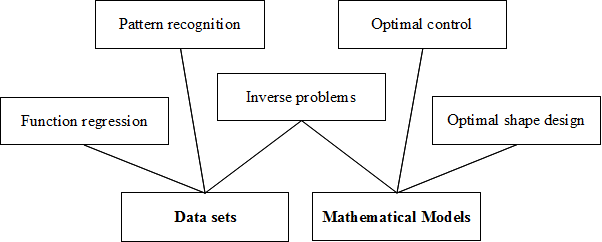
\includegraphics[width=1.0\textwidth]{neural_networks_basis/learning_tasks}
\caption{Learning tasks for neural networks.}\label{LearningTasksFigure}
\end{center}
\end{figure}


%%%%%%%%%%%%%%%%%%%%%%%%%%%%%%%%%%%%%%%%%%%%%%%%%%%%%%%%%%%%%%%%%%%%%%%%%%%%%%%%%%%%

\chapter{Software model basis}\label{SoftwareModelBasis}
In this Chapter we present the software model of \texttt{OpenNN}. 
The whole process is carried out in the Unified Modeling Language (UML).
The final implementation is written in the C++ Programming Language.

\section{Unified Modeling Language (UML)}

The Unified Modeling Language (UML) is a general purpose visual
modeling language that is used to specify, visualize, construct,
and document the artifacts of a software system
\cite{Rumbaugh1999}.

In order to construct a model for \texttt{OpenNN}, we
follow a top-down development. This approach to the problem begins
at the highest conceptual level and works down to the details. In
this way, to create and evolve a conceptual class diagram, we iteratively model:

\begin{enumerate}
\item Classes.
\item Associations.
\item Compositions.
\item Derived classes.
\item Members.
\item Methods.
\end{enumerate}

\section{Classes}\index{class, object oriented programming}

% Introduction

In colloquial terms a concept is an idea or a thing. In
object-oriented modeling concepts are represented by means of
classes \cite{Stroustrup2000}. Therefore, a prime task is to
identify the main concepts (or classes) of the problem domain. In
UML class diagrams, classes are depicted as boxes
\cite{Rumbaugh1999}.

% OpenNN

Through all this work, we have seen that general problemss can be solved 
with three elements: a neural network, a
performance functional and a training strategy. The characterization
in classes of these three concepts for \texttt{OpenNN} is
as follows:

\begin{description}

\item[NeuralNetwork] 

The class representing the concept of neural network is called \lstinline"NeuralNetwork".

\item[Performance functional]

The class which represents the concept of performance functional is called \lstinline"PerformanceFunctional".

\item[Training strategy]

The class representing the concept of training strategy is called \lstinline"TrainingStrategy".

\end{description}

Figure \ref{ConceptDiagram} depicts a starting UML class diagram
for the conceptual model of \texttt{OpenNN}.

\begin{figure}[h!]
\begin{center}
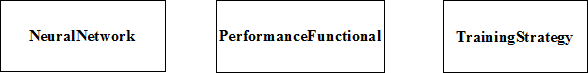
\includegraphics[width=0.975\textwidth]{software_model_basis/concept_diagram}
\caption{Conceptual diagram for \texttt{OpenNN}.}\label{ConceptDiagram}
\end{center}
\end{figure}


\section{Associations}
\index{association, object oriented programming}

% Introduction

Once identified the main concepts in the model it is necessary to
aggregate the associations among them. An association is a
relationship between two concepts which points some significative
or interesting information \cite{Stroustrup2000}. In UML class
diagrams, an association is shown as a line connecting two
classes. It is also possible to assign a label to an association.
The label is typically one or two words describing the association
\cite{Rumbaugh1999}.

% OpenNN

The appropriate associations among the main concepts of \texttt{OpenNN} are next identified to
be included to the UML class diagram of the system:

\begin{description}
\item[Neural network- Performance functional]
A neural network \textit{has assigned} a performance
functional.
\item[Performance functional - Training strategy]
A performance functional \textit{is improved by} a training
strategy.
\end{description}

Figure \ref{AssociationDiagram} shows the above UML class diagram
with these associations aggregated.

\begin{figure}[h!]
\begin{center}
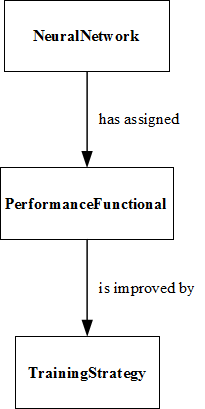
\includegraphics[width=0.35\textwidth]{software_model_basis/association_diagram}
\caption{Aggregation of associations to the conceptual diagram.}\label{AssociationDiagram}
\end{center}
\end{figure}

\section{Composition}

% Introduction

Classes are usually composed of another classes. The higher level classes manage the lower level ones. 

% OpenNN

Regarding \texttt{OpenNN}, the three main concepts described above are quite high level structures. 
This means that the neural network, performance functional and training algorithm classes are composed by different elements. 
In the next chapters the composition of the high level objects is explained in some detail. 

\section{Derived classes}\index{derived class, object oriented programming}

% Introduction

In object-oriented programming, some classes are designed only as
a parent from which sub-classes may be derived, but which is not
itself suitable for instantiation. This is said to be an
\textit{abstract class}\index{abstract class, object oriented
programming}, as opposed to a \textit{concrete
class}\index{concrete class, object oriented programming}, which
is suitable to be instantiated. The derived class contains all the
features of the base class, but may have new features added or
redefine existing features \cite{Stroustrup2000}. Associations
between a base class an a derived class are of the kind \textit{is
a} \cite{Rumbaugh1999}.

% OpenNN

Some \texttt{OpenNN} classes are abstract, and concrete classes are derived from them. 
In the next chapters we will describe the intheritance of the main components 
of \texttt{OpenNN}: the neural network, the performance functional and the training strategy.  

\section{Members and methods} 
\index{attribute, object oriented programming}
\index{operation, object oriented programming}

A member (or attribute) is a named value or relationship that exists for all or some instances of a class. 
A method (or operation) is a procedure associated with a class \cite{Stroustrup2000}. 
In UML class diagrams, classes are depicted as boxes with three sections: the
top one indicates the name of the class, the one in the middle
lists the attributes of the class, and the bottom one lists the
operations \cite{Rumbaugh1999}.

The main members and methodss of the different \texttt{OpenNN} classes are described throughout all this manual. 


%%%%%%%%%%%%%%%%%%%%%%%%%%%%%%%%%%%%%%%%%%%%%%%%%%%%%%%%%%%%%%%%%%%%%%%%%%%%%%%%%%%%

\chapter{Neural network}\label{NeuralNetwork}
The class of neural network implemented in \texttt{OpenNN} is based on the multilayer perceptron.  
That model is extended here to contain scaling, unscaling, bounding, probabilistic and conditions layers. 
A set of independent parameters associated to the neural network is also included here for convenience. 


\section{Basic theory}\label{NeuralNetworkBasicTheory}
As we saw in the previous chapter the performance functional has a performance
function associated. 
The performance function for a neural network can be visualized as a hypersurface,
with the parameters as coordinates, see Figure
\ref{PerformanceFunctionFigure}.

\begin{figure}[h!]
\begin{center}
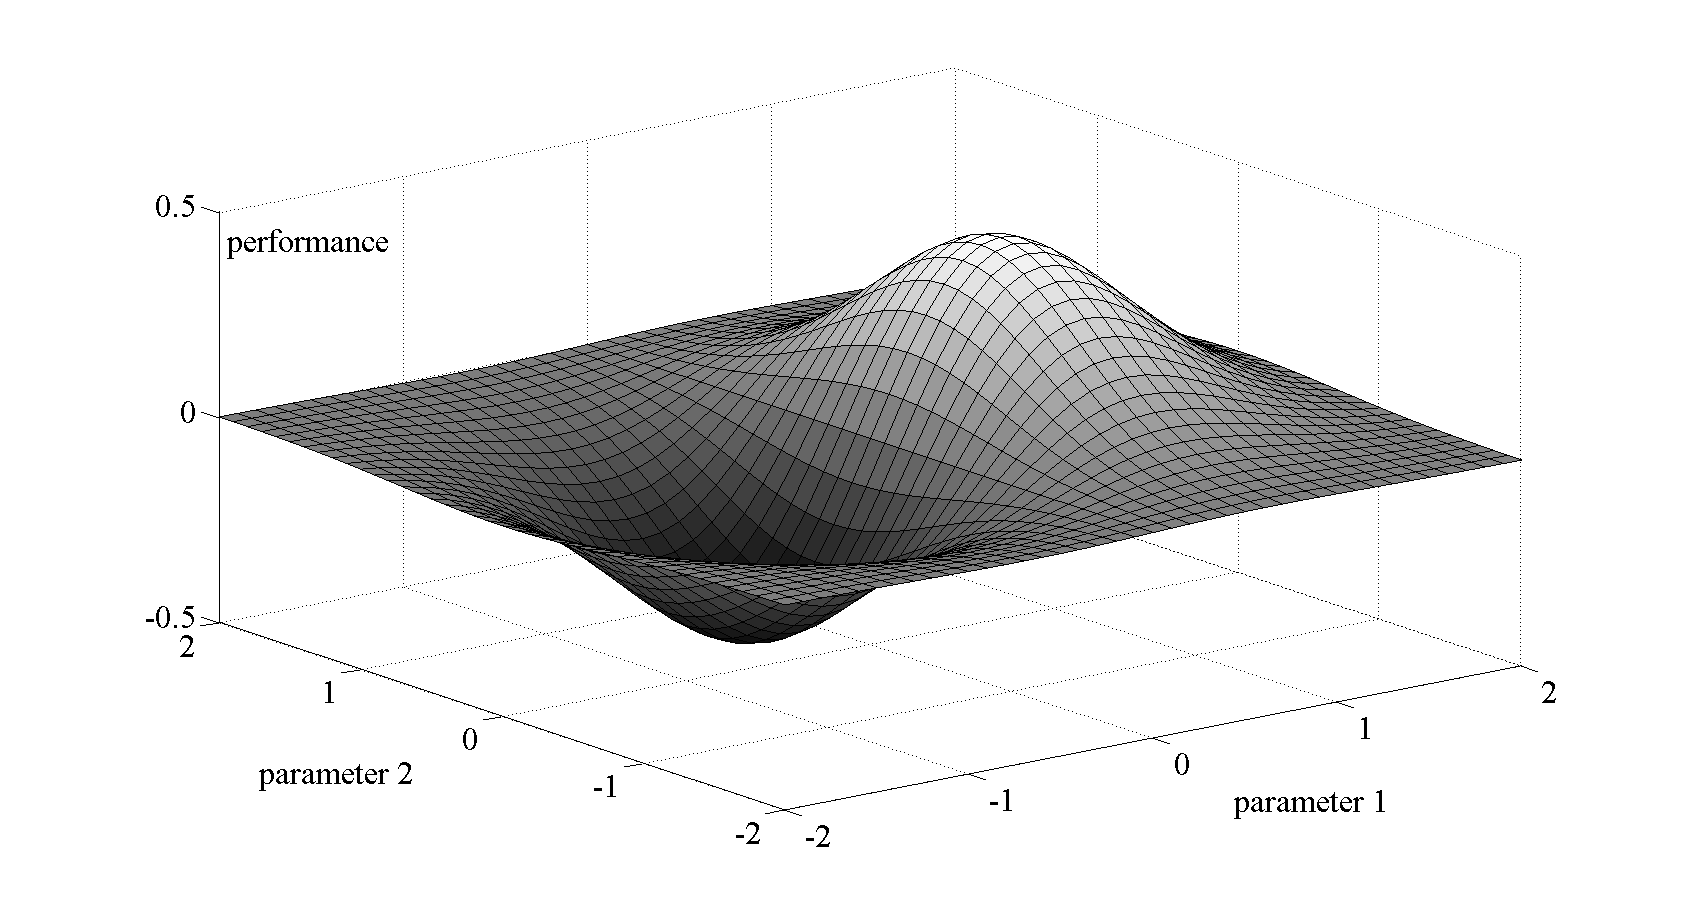
\includegraphics[width=1.0\textwidth]{training_strategy/performance_function.png}
\caption{Geometrical representation of the performance function.}\label{PerformanceFunctionFigure}
\end{center}
\end{figure}

The minimum or maximum value of the performance functional is
achieved for a vector of parameters at which the performance
function takes on a minimum or maximum value. Therefore, the
learning problem for neural networks, formulated as a
variational problem, can be reduced to a function optimization
problem \cite{Lopez2006ICANN}.

In this sense, a variational formulation for neural networks provides a direct method for solving variational 
problems. The universal approximation 
properties for the multilayer perceptron cause neural computation to
be a very appropriate paradigm for the solution of these problems.

\subsubsection{One-dimensional optimization}
\index{one dimensional optimization} 
\index{line search|see{one dimensional optimization}}

\index{relative minimum}
\index{local minimum}

\index{relative maximum}
\index{local maximum}

\index{absolute minimum}
\index{global minimum}

\index{absolute maximum}
\index{global maximum}

\index{first training rate}

Although the performance function is multidimensional, one-dimensional optimization methods are of great importance. 
Indeed, one-dimensional optimization algorithms are very often used inside multidimensional optimization algorithms. 

A function is said to have a relative or local minimum at some point if the function is always greater within some neighbourhood of that point. 
Similarly, a point is called a relative or local maximum if the function is always lesser within some neighbourhood of that point. 

The function is said to have a global or absolute minimum at some point if the function is always greater within the whole domain. 
Similarly, a point will be a global maximum if the function is always greater within the whole domain. 
Finding a global optimum is, in general, a very difficult problem \cite{Wolpert1997}. 

On the other hand, the tasks of maximization and minimization are trivially related to
each other, since maximization of a function is
equivalent to minimization of its negative, and vice
versa.

In this regard, a one-dimensional optimization problem is one in which the argument which minimizes the performance function is to be found. 

The necessary condition states that if the directional performance function has a relative optimum  and if the derivative exists as a finite number. 
The condition for the optimum to be a minimum is that the second derivative is greater than zero, and vice versa. 

The most elementary approach for one-dimensional optimization problems is to use a fixed step size or training rate. 
More sophisticated algorithms which are are widely used are the golden section method and the
Brent's method. Both of the two later algortims begin by bracketing a minimum. 

%\subsubsection{Fixed training rate}
%\index{fixed training rate}
%\index{fixed step size|see fixed training rate}

%The most elementary approach for such a problem is to use a fixed step size, or training rate, and move
%from an initial guess point in a favorable direction (positive or negative). The step size
%used must be small in relation to the final accuracy desired. Although this method is
%very simple to implement, it is not efficient in many cases.

The golden section method brackets that minimum until the distance
between the two outer points in the bracket is less than a defined
tolerance \cite{Press2002}.

The Brent's method performs a parabolic
interpolation until the distance between the two outer points
defining the parabola is less than a tolerance \cite{Press2002}.


\subsubsection{Multi-dimensional optimization}

\index{function optimization problem}
\index{performance function}
\index{global minimum, performance function}
\index{local minimum, performance function}

\index{global minimum condition}
\index{local minimum condition}

\index{epoch}
\index{iteration|see{epoch}}

\index{parameters increment}
\index{training direction}
\index{training rate}

\index{evaluation improvement}

\index{stopping criteria}

\index{minimum parameters increment norm}

\index{evaluation goal}
\index{minimum evaluation improvement}
\index{gradient norm goal}

\index{maximum time}
\index{maximum epochs number}

\index{early stopping}

\index{zero order method}
\index{random search}
\index{evolutionary algorithm}
\index{genetic algorithm|see{evolutionary algorithm}}

\index{first order method}
\index{gradient descent method}
\index{conjugate gradient method}
\index{scaled conjugate gradient}
\index{quasi-Newton method} 

\index{second order method}
\index{Newton's method}
\index{Levenberg-Marquardt algorithm}

As it was shown in Chapter \ref{PerformanceFunctional}, the learning problem for neural networks is reduced 
to the searching for a parameter vector at which the performance function takes
a maximum or a minimum value.

The concepts of relative or local and absolute or global optima for the multidimensional case apply in the same way as for the one-dimensional case. The tasks of maximization and minimization are also trivially related here. 

The necessary condition states that if the neural network is at a minimum of the performance function, 
then the gradient is the zero vector. 

The performance function is, in general, a non linear function of the
parameters. As a consequence, it is not possible to find closed
training algorithms for the minima. Instead, we consider a search
through the parameter space consisting of a succession of steps, or
epochs. 

At each epoch, the performance will increase by adjusting the neural network parameters. 
The change of parameters between two epochs is called the parameters increment. 

In this way, to train a neural network we start with some parameters vector 
(often chosen at random) and we generate a sequence of parameter vectors, so
that the performance function is reduced at each iteration of the algorithm. 
The change of performance between two epochs is called the performance improvement. 

The training algorithm stops when a specified condition is satisfied. 
Some stopping criteria commonly used are \cite{Demuth2009}:

\begin{enumerate}
\item The parameters increment norm is less than a minimum value. 
\item The performance improvement in one epoch is less than a set value.
\item Performance has been minimized to a goal value.
\item The norm of the performance function gradient falls below a goal.
\item A maximum number of epochs is reached.
\item A maximum amount of computing time has been exceeded.
\end{enumerate}

A stopping criterium of different nature is early stopping. 
This method is used in ill-possed problems in order to control the effective complexity of the neural network. 
Early stopping is a very common practice in neural networks and often produces good solutions to ill-possed problems. 

Figure \ref{TrainingProcess} is a state diagram of the training
procedure, showing states and transitions in the training process
of a neural network.

\begin{figure}[h!]
\begin{center}
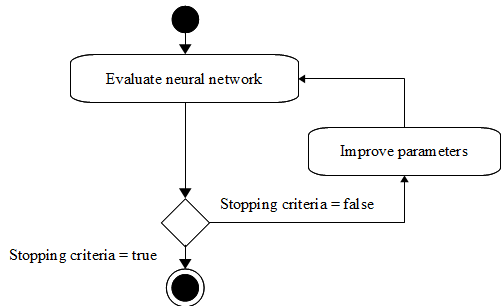
\includegraphics[width=0.8\textwidth]{training_strategy/training_process.png}
\caption{Training process.}\label{TrainingProcess}
\end{center}
\end{figure}

The training process is determined by the way in which the
adjustment of the parameters in the neural network takes place.
There are many different training algorithms, which have a variety
of different computation and storage requirements. Moreover, there
is not a training algorithm best suited to all locations
\cite{Wolpert1997}.

Training algorithms might require information from the performance
function only, the gradient vector of the performance function or the
Hessian matrix of the performance function \cite{Press2002}. These
methods, in turn, can perform either global or local optimization.

Zero-order training algorithms make use of the performance function
only. The most significant zero-order
training algorithms are stochastic, which involve randomness in the
optimization process. Examples of these are random
search and evolutionary
algorithms \cite{Goldberg1988}
\cite{Fogel1994} or particle swarm optimization \cite{Kennedy1995},
which are global optimization methods .

First-order training algorithms use the performance function and its
gradient vector \cite{Battiti1992}.
Examples of these are gradient descent methods, conjugate gradient methods, scaled conjugate gradient methods \cite{Moller1993} or quasi-Newton
methods. Gradient descent, conjugate
gradient, scaled conjugate gradient and quasi-Newton methods are
local optimization methods \cite{Luenberger1984}.

Second-order training algorithms make use of the performance function,
its gradient vector and its Hessian matrix \cite{Battiti1992}. Examples for second-order methods are
Newton's method and the Levenberg-Marquardt
algorithm \cite{Hagan1994}.
Both of them are local optimization methods \cite{Luenberger1984}.

\subsubsection{Training strategy}

Most of the times, application of a single training algorithm is enough to properly train a neural network. 
The quasi-Newton method is in general a good choice, since it provides good training times and deals successfully with most of the performance functions. 
The Levenberg-Marquardt algorithm could be also recommended for small and medium-sized data modelling problems. 
 
However, some applications might need more training effort. 
In that cases we can combine different algorithms in order to do our best. 
In problems defined by mathematical models, with constraints, etc. a single training algorithm might fail. 

Therefore, for difficult problems, we can try two use two or three different training algorithms. 
A general strategy consists on applying three different training algorithms: 

\begin{enumerate}
\item Initialization training algorithm. 
\item Main training algorithm. 
\item Refinement training algorithm. 
\end{enumerate}

The initialization training algorithm is used to bring the neural network to a stable region of the performance function.
Near the optimum, the performance function usually behaves better than far away. 
Zero order training algorithms, such as random search or the evolutionary algorithm might good for this initialization process. 
Indeed, they are very robust algorithms. 

The main training algorithm does most of the job. The training strategy relies on them. 
First order training algorithms, such as the quasi-Newton method are a good choce here. 

Finally, a refinement training algorithm can be used when a big accuracy is required. 
Second orden training algorithms, such as the Newton-method, require the most exact information of the performance function. Therefore they can perform better for refinement. 



\section{Software model}\label{NeuralNetworkSoftwareModel}
%\section{Derived classes}\index{derived class, object oriented programming}

As we have seen, the \texttt{OpenNN} neural network is composed by a multilayer perceptron plus some other kinds of layers. 
In this section we study the software model of the \lstinline"NeuralNetwork" class. 


\subsection*{Classes}

The characterization in classes of the concepts studied in the previous section is as follows:

\begin{description}

\item[Perceptron] The class which represents the concept of perceptron neuron model is called \lstinline"Perceptron".

\item[PerceptronLayer] The class representing a layer of perceptrons is called \lstinline"PerceptronLayer".

\item[MultilayerPerceptron] The class which represents a feed-forward architecture of perceptron layers is called \lstinline"MultilayerPerceptron".

\item[Scaling layer] The class which represents a layer for scaling variables is called \lstinline"ScalingLayer".

\item[Unscaling layer] The class which represents an unscaling layer is called \lstinline"UnscalingLayer".
 
\item[Bounding layer] The class representing a layer of bounding neurons is called \lstinline"BoundingLayer".

\item[Conditions layer] The class wich applies input-output conditions is called \lstinline"ConditionsLayer".

\item[Independent parameters] A class containing parameters not belonging to the multilayer perceptron is called \lstinline"IndependentParameters".

\item[Neural network] The class which aggregates all the different neural network concepts is called \lstinline"NeuralNetwork".

\end{description}

\subsection*{Associations}

The appropriate associations between all the neural networks classes in the system are next identified to be included
to the association diagram:

\begin{description}

\item[Perceptron layer - perceptron] A layer of perceptrons is composed of perceptrons.

\item[Multilayer perceptron - perceptron layer] A multilayer perceptron is composed of layers of perceptrons.

\item[Neural network - Multilayer perceptron] A neural network very probably contains a multilayer perceptron.

\item[Neural network - Scaling layer] A multilayer perceptron usually contains a scaling layer. 

\item[Neural network - Unscaling layer] A multilayer perceptron usually contains an unscaling layer. 

\item[Neural network - Bounding layer] A multilayer perceptron sometimes contains a bounding layer.

\item[Neural network - Probabilistic layer] A multilayer perceptron sometimes contains a probabilistic layer.

\item[Neural network - Conditions layer] A multilayer perceptron might contain a conditions layer.

\item[Neural network - Independent parameters] A multilayer percetpron might contain a set of independent parameters.    

\end{description}

Figure \ref{NeuralNetworkAssociationDiagram} depicts an association diagram
for the neural network class. 

\begin{figure}[h!]
\begin{center}
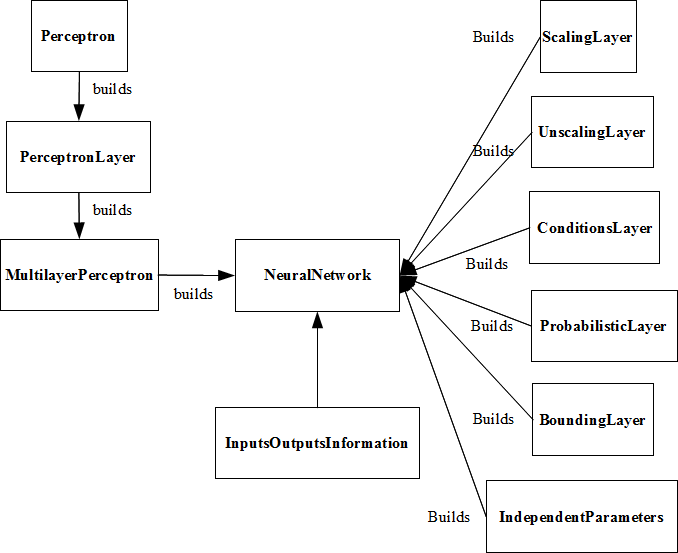
\includegraphics[width=1.1\textwidth]{neural_network/association_diagram}
\caption{Association diagram for the \lstinline'NeuralNetwork' class.}\label{NeuralNetworkAssociationDiagram}
\end{center}
\end{figure}

\subsection*{Derived classes}

The next task is then to establish which classes are abstract and
to derive the necessary concrete classes to be added to the
system. 

The neural network class in \texttt{OpenNN} will be intensively used by any application. 
Therefore, for performance reasons, all the composing classes have been designed to be concrete. 

Let us then examine the classes we have so far:

\begin{description}

\item[Perceptron] The class \lstinline"Perceptron" is concrete,
and can implement different activation functions. 

\item[Perceptron layer] The class \lstinline"PerceptronLayer" is also concrete,
since it is defined as a vector of perceptrons.

\item[Multilayer perceptron] The class \lstinline"MultilayerPerceptron" is a concrete class and is
itself suitable for instantiation. This class is implemented as a vector of layers of perceptrons. 

\item[Scaling layer] The class \lstinline"ScalingLayer" is concrete, and implements the minimum-maximum and mean-standard deviation scaling methods.

\item[Unscaling layer] The class \lstinline"UnscalingLayer" is also concrete, and implements the minimum-maximum and mean-standard deviation unscaling methods.

\item[Bounding layer] The class \lstinline"BoundingLayer" is concrete. It sets to their bound values those inputs which are below or above them. 

\item[Probabilistic layer] The class \lstinline"ProbabilisticLayer" is concrete, and implements the competitive and softmax methods.

\item[Conditions layer] The class \lstinline"ConditionsLayer" has also been designed to be concrete. It implements methods to hold one or two condions. For more difficult situations, further classes must be derived. 

\item[Inputs-outputs information] The class \lstinline"InputsOutputsInformation" is concrete. It mainly stores a few strings with the names, units and descriptions of the neural network variables. 

\item[Independent parameters] The class \lstinline"IndependentParameters" is concrete. It contains other adjustable parameters 
than those belonging to the multilayer perceptron. 

\end{description}

\subsection*{Attributes and operations}

An attribute is a named value or relationship that exists for all
or some instances of a class. An operation is a procedure
associated with a class \cite{Stroustrup2000}. 

In UML class
diagrams, classes are depicted as boxes with three sections: the
top one indicates the name of the class, the one in the middle
lists the attributes of the class, and the bottom one lists the
operations \cite{Rumbaugh1999}.


\begin{description}

\item[Perceptron] A perceptron neuron model has the following attributes:

\begin{itemize}
\item[-] A bias.
\item[-] A set of synaptic weights.
\item[-] The activation function.
\end{itemize}

It performs the following main operations:

\begin{itemize}
\item[-] Calculate the neuron output for a given input.
\item[-] Calculate the derivatives of the output with respect to the inputs.
\end{itemize}


\item[Perceptron layer] The perceptron layer has the following members:

\begin{itemize}
\item[-] A set of perceptrons.
\end{itemize}
 
It performs the following methods:

\begin{itemize}
\item[-] Calculate the layer output for a given input.
\item[-] Calculate the derivatives of the outputs with respect to the inputs.
\end{itemize}

\item[Multilayer perceptron] A multilayer perceptron has the following attributes:

\begin{itemize}
\item[-] A set of layers of perceptrons.
\end{itemize}

It performs the following main operations:

\begin{itemize}
\item[-] Calculate the output for a given input.
\item[-] Calculate the Jacobian for a given input.
\item[-] Calculate the Hessian form for a given input.
\end{itemize}

\item[Scaling layer] The scaling layer has the following members:

\begin{itemize}
\item[-] The main statistics of the variables.
\item[-] The scaling method.
\end{itemize}

It implements the following main members:

\begin{itemize}
\item[-] Calculate the scaled variables for unscaled variables.
\item[-] Calculate the derivatives of the scaling function.
\end{itemize}

\item[Unscaling layer] The unscaling layer is similar to the scaling layer, 
with the following members:

\begin{itemize}
\item[-] The main statistics of the variables.
\item[-] The unscaling method.
\end{itemize}

It implements the following main members:

\begin{itemize}
\item[-] Calculate the unscaled variables for scaled variables.
\item[-] Calculate the derivatives of the unscaling function.
\end{itemize}

\item[Bounding layer] The bounding layer contains the following attributes:

\begin{itemize}
\item[-] The lower and upper bounds of the variables.
\end{itemize}

It performs the following main operations:

\begin{itemize}
\item[-] Calculate bounded variables for unbounded ones.
\item[-] Calculate the derivatives of the bounding function.
\end{itemize}

\item[Probabilistic layer] The probabilist layer contains:

\begin{itemize}
\item[-] The probabilistic method.
\end{itemize}

It computes the following functions:

\begin{itemize}
\item[-] Calculate probabilistic variables for non-probabilistic ones.
\item[-] Calculate also the derivatives.
\end{itemize}

\item[Conditions layer] The conditions layer contains the following:

\begin{itemize}
\item[-] The conditions values.
\item[-] The conditions method.
\end{itemize}

   
It performs the following:

\begin{itemize}
\item[-] Calculate outputs holding some conditions. 
\item[-] Calculate also the derivatives of that conditioned outputs.
\end{itemize}

\item[Inputs-outputs information] This class stores the following data:

\begin{itemize}
\item[-] The names, units and descriptions of the input and output variables.
\end{itemize}

It performs the following:

\begin{itemize}
\item[-] Write default names for the inputs and the outputs. 
\end{itemize}

\item[Independent parameters] The class representing independent parameters contains the following main members:

\begin{itemize}
\item[-] A set of parameters.
\item[-] Information and statistics on the parameters.
\item[-] Scaling/Unscaling and bounding methods. 
\end{itemize}

The independent parameters class can perform the follwoing operations:

\begin{itemize}
\item[-] Scale and unscale the parameters.
\item[-] Bounding the parameters. 
\end{itemize}

\end{description}





\section{NeuralNetwork classes}\label{NeuralNetworkClassese}
\index{NeuralNetwork class}

As it has been said, \texttt{OpenNN} implements quite a general neural network in the class \lstinline"NeuralNetwork". 
It contains a multilayer perceptron with an arbitrary number of layers of perceptrons. 
On the other hand, it includes aditional layers for inputs scaling, outputs unscaling, outputs bouding, outputs probabilizing
or outputs holding some other conditions. 
This neural network can deal with a wide range of problems. 
Finally this class includes independent parameters, which can be useful for some problems. 

The \lstinline"NeuralNetwork" class is one of the most important in \texttt{OpenNN}, having many different members, constructors and methods. 

\subsection*{Members}

The \lstinline"NeuralNetwork" class contains:

\begin{itemize}
\item[-] A pointer to a multilayer perceptron.
\item[-] A pointer to a scaling layer.
\item[-] A pointer to an unscaling layer.
\item[-] A pointer to a bounding layer.
\item[-] A pointer to a probabilistic layer.
\item[-] A pointer to a conditions layer.
\item[-] A pointer to an inputs-outputs information object.
\item[-] A pointer to a set of independent parameters.
\end{itemize}

All that members are declared as private, and they can only be used with their corresponding get or set methods. 

\subsection*{Constructors}

There are several constructors for the \lstinline"NeuralNetwork" class, with different arguments. 

The default activation function for the hidden layers is the hyperbolic tangent, and for the output layer is the linear. No default information, statistics, scaling, boundary conditions or bounds are set.

% Default constructor

The easiest way of creating a neural object is by means of the default constructor, which creates an empty neural network. 

\begin{lstlisting}
NeuralNetwork nn;
\end{lstlisting}

% One layer constructor

To construct neural network having a multilayer perceptron with, for example, $3$
inputs and $2$ output neurons, we use the one layer constructor

\begin{lstlisting}
NeuralNetwork nn(3, 2);
\end{lstlisting}

All the parameters in the multilayer perceptron object that
we have constructed so far are initialized with random values chosen
from a normal distribution with mean $0$ and standard deviation $1$.
By default, this one-layer perceptron will have linear activation function.

% One hidden layer constructor

To construct a neural network containing a multilayer perceptron object with, for example, $1$
input, a single hidden layer of $3$ neurons and an output layer with
$2$ neurons, we use the two layers constructor

\begin{lstlisting}
NeuralNetwork nn(1,6,2);
\end{lstlisting}

All the parameters here are also initialized at random. 
By default, the hidden layer will have hyperbolic tangent activation function 
and the output layer will have linear activation function.

% Architecture constructor 

In order to construct a neural network with a more complex multilayer perceptron,
its architecture must be specified in a vector of unsigned integers. 
For instance, to construct a multilayer
perceptron with $1$ input, $3$ hidden layers with $2$, $4$ and $3$ neurons and
an output layer with $1$ neuron we can write

\begin{lstlisting}
Vector<unsigned int> architecture(5);
architecture[0] = 1;
architecture[1] = 2;
architecture[2] = 4;
architecture[3] = 3;
architecture[4] = 1;

NeuralNetwork nn(architecture);
\end{lstlisting}

The network parameters here are also initialized at random. 

% Independent parameters constructor

The independent parameters constructor creates a neural network object without a multilayer perceptron but with a given number of independent parameters, 

\begin{lstlisting}
NeuralNetwork nn(3);
\end{lstlisting}

The above object can be used, for instance, as the basis for solving a function optimization problem not related to neural networks. 

% File constructor

It is possible to construct a neural network by loading its members from a XML file. 
That is done in the following way, 

\begin{lstlisting}
NeuralNetwork nn(`neural_network.xml');
\end{lstlisting}

Please follow strictly the format of the neural network file. 

% Copy constructor

Finally, the copy constructor can be used to create an object by copying the members from another object, 

\begin{lstlisting}
NeuralNetwork nn1(2, 4, 3);
NeuralNetwork nn2(&nn1);
\end{lstlisting}

\subsection*{Methods}

This class implements get and set methods for each member. 
The following sentences show the use of some of them,

\begin{lstlisting}
NeuralNetwork nn(3, 2);

MultilayerPerceptronPointer* mlpp = nn.get_multilayer_perceptron_pointer();

unsigned int inputs_number = mlpp.count_inputs_number();
unsigned int outputs_number = mlpp.count_outputs_number();

\end{lstlisting}

% Get methods

The number of parameters of the neural network above can be accessed as follows

\begin{lstlisting}
unsigned int parameters_number = nn.count_parameters_number();
\end{lstlisting}

% Initialization methods

The network parameters can be initialized with a given value by using the \lstinline"initialize" method, 

\begin{lstlisting}
NeuralNetwork nn(4, 3, 2);

nn.initialize(0.0);
\end{lstlisting}

% Parameters norm methods

% Output methods

To calculate the output \lstinline"Vector" of the network in
response to an input \lstinline"Vector" we use the method
\lstinline"calculate_outputs". For instance, the
sentence

\begin{lstlisting}
Vector<double> inputs(1); 
inputs[0] = 0.5;

Vector<double> outputs = nn.calculate_outputs(inputs);
\end{lstlisting}

\noindent returns the neural network output value for an input value.

% Jacobian matrix methods

To calculate the Jacobian \lstinline"Matrix" of the network in
response to an input \lstinline"Vector" we use the method  the
method \lstinline"calculate_Jacobian". For instance,
the sentence

\begin{lstlisting}
Matrix<double> Jacobian = nn.calculate_Jacobian(inputs);
\end{lstlisting}

\noindent returns the partial derivatives of the outputs with respect to the inputs.

% Sensitivity matrix methods 

% Independent parameters methods

% Serialization methods

We can save a neural network object to a data file by using the method \lstinline"save". For instance,

\begin{lstlisting}
NeuralNetwork nn;

nn.save(`neural_network.xml');
\end{lstlisting}

\noindent saves the neural network object to the file \lstinline"neural_network.xml".

We can also load a neural network object from a data file by
using the method  \lstinline"load". Indeed, the sentence

\begin{lstlisting}
nn.load(`neural_network.xml');
\end{lstlisting}

\noindent loads the neural network object from the file \lstinline"neural_network.xml".

\subsection*{XML formats}

\subsubsection*{Multilayer perceptron}

The format of a XML multilayer perceptron element is the following,

\begin{lstlisting}
<MultilayerPerceptron>
   <Architecture>vector</Architecture>
   <Parameters>vector</Parameters>
   <ActivationFunctions>vector</ActivationFunctions>
   <Display>bool</Display>
</MultilayerPerceptron>
\end{lstlisting}

\subsubsection*{Scaling layer}

The format of a XML scaling layer element is the following,

\begin{lstlisting}
<ScalingLayer>
   <Minimums>vector</Minimums>
   <Maximums>vector</Maximums>
   <Means>vector</Means>
   <StandardDeviations>vector</StandardDeviations>
   <ScalingMethod>string</ScalingMethod>
   <Display>bool</Display>
</ScalingLayer>
\end{lstlisting}

\subsubsection*{Unscaling layer}

The format of a XML unscaling layer element is the following,

\begin{lstlisting}
<UnscalingLayer>
   <Minimums>vector</Minimums>
   <Maximums>vector</Maximums>
   <Means>vector</Means>
   <StandardDeviations>vector</StandardDeviations>
   <UnscalingMethod>string</UnscalingMethod>
   <Display>bool</Display>
</UnscalingLayer>
\end{lstlisting}

\subsubsection*{Bounding layer}

The format of a XML bounding layer element is the following,

\begin{lstlisting}
<BoundingLayer>
   <LowerBounds>vector</LowerBounds>
   <UpperBounds>vector</UpperBounds>
   <Display>bool</Display>
</BoundingLayer>
\end{lstlisting}


\subsubsection*{Probabilistic layer}

The format of a XML probabilistic layer element is the following,

\begin{lstlisting}
<ProbabilisticLayer>
   <ProbabilisticNeuronsNumber>integer</ProbabilisticNeuronsNumber>
   <ProbabilisticMethod>string</ProbabilisticMethod>
   <Display>bool</Display>
</ProbabilisticLayer>
\end{lstlisting}


\subsubsection*{Conditions layer}

The format of a XML conditions layer element is the following,

\begin{lstlisting}
<ConditionsLayer>
   <InputsNumber>integer</InputsNumber>
   <ConditionsNeuronsNumber>integer</ConditionsNeuronsNumber>
   <ConditionsMethod>string</ConditionsMethod>
   <Display>bool</Display>
</ConditionsLayer>
\end{lstlisting}

\subsubsection*{Inputs-outputs information}

\begin{lstlisting}
<InputsOutputsInformation>
   <InputsName>
      <InputName Index="1">string</InputName>
      ...
      <InputName Index="N">string</InputName>   
   </InputsName>
   <InputsUnits>
      <InputUnits Index="1">string</InputUnits>
      ...
      <InputUnits Index="N">string</InputUnits>   
   </InputsUnits>
   <InputsDescription>
      <InputDescription Index="1">string</InputDescription>
      ...
      <InputDescription Index="N">string</InputDescription>   
   </InputsDescription>
   <OutputsName>
      <OutputName Index="1">string</OutputName>
      ...
      <OutputName Index="N">string</OutputName>   
   </OutputsName>
   <OutputsUnits>
      <OutputUnits Index="1">string</OutputUnits>
      ...
      <OutputUnits Index="N">string</OutputUnits>   
   </OutputsUnits>
   <OutputsDescription>
      <OutputDescription Index="1">string</OutputDescription>
      ...
      <OutputDescription Index="M">string</OutputDescription>   
   </OutputsDescription>
</InputsOutputsInformation>
\end{lstlisting}

\subsubsection*{Independent parameters}

The format of a XML independent parameters element is the following,

\begin{lstlisting}
<IndependentParameters>
   <Parameters>vector</Parameters>
   <Names> 
      <Name Index="1">string</Name>
      ...
      <Name Index="NIP">string</Name>   
   </Names> 
   <Units> 
      <Unit Index="1">string</Unit>
      ...
      <Unit Index="NIP">string</Unit>   
   </Units> 
   <Descriptions> 
      <Description Index="1">string</Description>
      ...
      <Description Index="NIP">string</Description>   
   </Units> 
   <Minimums>vector</Minimums>
   <Maximums>vector</Maximums>
   <Means>vector</Means>
   <StandardDeviations>vector</StandardDeviations>
   <LowerBounds>vector</LowerBounds>
   <UpperBounds>vector</UpperBounds>
   <ScalingMethod>string</ScalingMethod>
   <ScalingFlag>boolean</ScalingFlag>
   <BoundingFlag>boolean</BoundingFlag>
   <DisplayRangeWarning>bool</DisplayRangeWarning>
   <Display>bool</Display>
</IndependentParameters>
\end{lstlisting}


\subsubsection*{Neural network}

Finally, the format of a XML independent parameters element is the following,

\begin{lstlisting}
<NeuralNetwork>
   <MultilayerPerceptron>
   multilayer_perceptron_element
   </MultilayerPerceptron>
   <ScalingLayer>
   scaling_layer_element
   </ScalingLayer>
   <UnscalingLayer>
   unscaling_layer_element
   </UnscalingLayer>
   <BoundingLayer>
   bounding_layer_element
   </BoundingLayer>
   <ProbabilisticLayer>
   probabilistic_layer_element
   </ProbabilisticLayer>
   <ConditionsLayer>
   conditions_layer_element
   </ConditionsLayer>
   <MultilayerPerceptronFlag>
   bool
   </MultilayerPerceptronFlag>
   <ScalingLayerFlag>
   bool
   </ScalingLayerFlag>
   <UnscalingLayerFlag>
   bool
   </UnscalingLayerFlag>
   <BoundingLayerFlag>
   bool
   </BoundingLayerFlag>
   <ProbabilisticLayerFlag>
   bool
   </ProbabilisticLayerFlag>
   <ConditionsLayerFlag>
   bool
   </ConditionsLayerFlag>
   <Display>
   bool
   </Display>
</NeuralNetwork>
\end{lstlisting}



%%%%%%%%%%%%%%%%%%%%%%%%%%%%%%%%%%%%%%%%%%%%%%%%%%%%%%%%%%%%%%%%%%%%%%%%%%%%%%%%%%%%
 
\chapter{Performance functional}\label{PerformanceFunctional}
\index{performance functional class}

The performance functional defines the learning task for a neural network. 
In \texttt{OpenNN}, a performance functional consists of three different terms: objective, 
regularization and constraints.




\section{Basic theory}\label{PerformanceFunctionalBasicTheory}
As we saw in the previous chapter the performance functional has a performance
function associated. 
The performance function for a neural network can be visualized as a hypersurface,
with the parameters as coordinates, see Figure
\ref{PerformanceFunctionFigure}.

\begin{figure}[h!]
\begin{center}
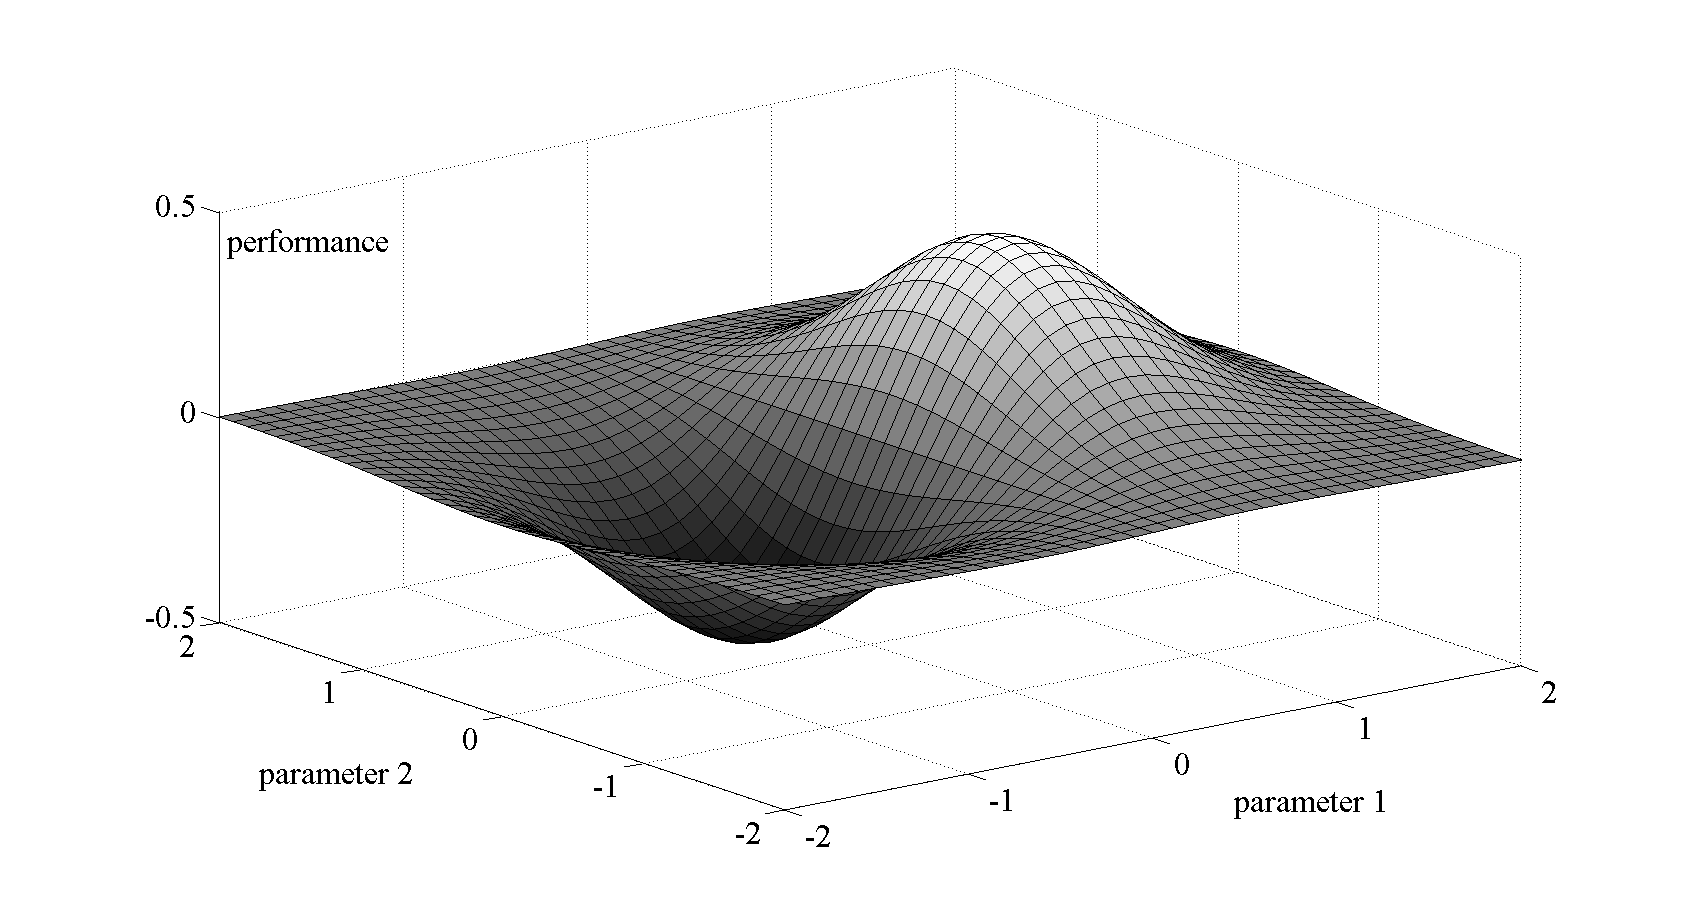
\includegraphics[width=1.0\textwidth]{training_strategy/performance_function.png}
\caption{Geometrical representation of the performance function.}\label{PerformanceFunctionFigure}
\end{center}
\end{figure}

The minimum or maximum value of the performance functional is
achieved for a vector of parameters at which the performance
function takes on a minimum or maximum value. Therefore, the
learning problem for neural networks, formulated as a
variational problem, can be reduced to a function optimization
problem \cite{Lopez2006ICANN}.

In this sense, a variational formulation for neural networks provides a direct method for solving variational 
problems. The universal approximation 
properties for the multilayer perceptron cause neural computation to
be a very appropriate paradigm for the solution of these problems.

\subsubsection{One-dimensional optimization}
\index{one dimensional optimization} 
\index{line search|see{one dimensional optimization}}

\index{relative minimum}
\index{local minimum}

\index{relative maximum}
\index{local maximum}

\index{absolute minimum}
\index{global minimum}

\index{absolute maximum}
\index{global maximum}

\index{first training rate}

Although the performance function is multidimensional, one-dimensional optimization methods are of great importance. 
Indeed, one-dimensional optimization algorithms are very often used inside multidimensional optimization algorithms. 

A function is said to have a relative or local minimum at some point if the function is always greater within some neighbourhood of that point. 
Similarly, a point is called a relative or local maximum if the function is always lesser within some neighbourhood of that point. 

The function is said to have a global or absolute minimum at some point if the function is always greater within the whole domain. 
Similarly, a point will be a global maximum if the function is always greater within the whole domain. 
Finding a global optimum is, in general, a very difficult problem \cite{Wolpert1997}. 

On the other hand, the tasks of maximization and minimization are trivially related to
each other, since maximization of a function is
equivalent to minimization of its negative, and vice
versa.

In this regard, a one-dimensional optimization problem is one in which the argument which minimizes the performance function is to be found. 

The necessary condition states that if the directional performance function has a relative optimum  and if the derivative exists as a finite number. 
The condition for the optimum to be a minimum is that the second derivative is greater than zero, and vice versa. 

The most elementary approach for one-dimensional optimization problems is to use a fixed step size or training rate. 
More sophisticated algorithms which are are widely used are the golden section method and the
Brent's method. Both of the two later algortims begin by bracketing a minimum. 

%\subsubsection{Fixed training rate}
%\index{fixed training rate}
%\index{fixed step size|see fixed training rate}

%The most elementary approach for such a problem is to use a fixed step size, or training rate, and move
%from an initial guess point in a favorable direction (positive or negative). The step size
%used must be small in relation to the final accuracy desired. Although this method is
%very simple to implement, it is not efficient in many cases.

The golden section method brackets that minimum until the distance
between the two outer points in the bracket is less than a defined
tolerance \cite{Press2002}.

The Brent's method performs a parabolic
interpolation until the distance between the two outer points
defining the parabola is less than a tolerance \cite{Press2002}.


\subsubsection{Multi-dimensional optimization}

\index{function optimization problem}
\index{performance function}
\index{global minimum, performance function}
\index{local minimum, performance function}

\index{global minimum condition}
\index{local minimum condition}

\index{epoch}
\index{iteration|see{epoch}}

\index{parameters increment}
\index{training direction}
\index{training rate}

\index{evaluation improvement}

\index{stopping criteria}

\index{minimum parameters increment norm}

\index{evaluation goal}
\index{minimum evaluation improvement}
\index{gradient norm goal}

\index{maximum time}
\index{maximum epochs number}

\index{early stopping}

\index{zero order method}
\index{random search}
\index{evolutionary algorithm}
\index{genetic algorithm|see{evolutionary algorithm}}

\index{first order method}
\index{gradient descent method}
\index{conjugate gradient method}
\index{scaled conjugate gradient}
\index{quasi-Newton method} 

\index{second order method}
\index{Newton's method}
\index{Levenberg-Marquardt algorithm}

As it was shown in Chapter \ref{PerformanceFunctional}, the learning problem for neural networks is reduced 
to the searching for a parameter vector at which the performance function takes
a maximum or a minimum value.

The concepts of relative or local and absolute or global optima for the multidimensional case apply in the same way as for the one-dimensional case. The tasks of maximization and minimization are also trivially related here. 

The necessary condition states that if the neural network is at a minimum of the performance function, 
then the gradient is the zero vector. 

The performance function is, in general, a non linear function of the
parameters. As a consequence, it is not possible to find closed
training algorithms for the minima. Instead, we consider a search
through the parameter space consisting of a succession of steps, or
epochs. 

At each epoch, the performance will increase by adjusting the neural network parameters. 
The change of parameters between two epochs is called the parameters increment. 

In this way, to train a neural network we start with some parameters vector 
(often chosen at random) and we generate a sequence of parameter vectors, so
that the performance function is reduced at each iteration of the algorithm. 
The change of performance between two epochs is called the performance improvement. 

The training algorithm stops when a specified condition is satisfied. 
Some stopping criteria commonly used are \cite{Demuth2009}:

\begin{enumerate}
\item The parameters increment norm is less than a minimum value. 
\item The performance improvement in one epoch is less than a set value.
\item Performance has been minimized to a goal value.
\item The norm of the performance function gradient falls below a goal.
\item A maximum number of epochs is reached.
\item A maximum amount of computing time has been exceeded.
\end{enumerate}

A stopping criterium of different nature is early stopping. 
This method is used in ill-possed problems in order to control the effective complexity of the neural network. 
Early stopping is a very common practice in neural networks and often produces good solutions to ill-possed problems. 

Figure \ref{TrainingProcess} is a state diagram of the training
procedure, showing states and transitions in the training process
of a neural network.

\begin{figure}[h!]
\begin{center}
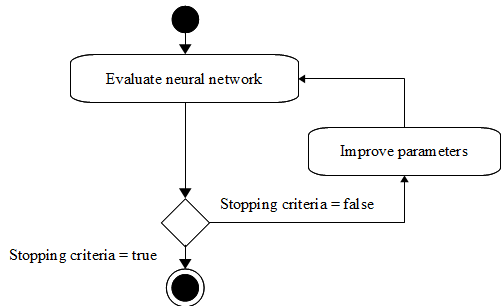
\includegraphics[width=0.8\textwidth]{training_strategy/training_process.png}
\caption{Training process.}\label{TrainingProcess}
\end{center}
\end{figure}

The training process is determined by the way in which the
adjustment of the parameters in the neural network takes place.
There are many different training algorithms, which have a variety
of different computation and storage requirements. Moreover, there
is not a training algorithm best suited to all locations
\cite{Wolpert1997}.

Training algorithms might require information from the performance
function only, the gradient vector of the performance function or the
Hessian matrix of the performance function \cite{Press2002}. These
methods, in turn, can perform either global or local optimization.

Zero-order training algorithms make use of the performance function
only. The most significant zero-order
training algorithms are stochastic, which involve randomness in the
optimization process. Examples of these are random
search and evolutionary
algorithms \cite{Goldberg1988}
\cite{Fogel1994} or particle swarm optimization \cite{Kennedy1995},
which are global optimization methods .

First-order training algorithms use the performance function and its
gradient vector \cite{Battiti1992}.
Examples of these are gradient descent methods, conjugate gradient methods, scaled conjugate gradient methods \cite{Moller1993} or quasi-Newton
methods. Gradient descent, conjugate
gradient, scaled conjugate gradient and quasi-Newton methods are
local optimization methods \cite{Luenberger1984}.

Second-order training algorithms make use of the performance function,
its gradient vector and its Hessian matrix \cite{Battiti1992}. Examples for second-order methods are
Newton's method and the Levenberg-Marquardt
algorithm \cite{Hagan1994}.
Both of them are local optimization methods \cite{Luenberger1984}.

\subsubsection{Training strategy}

Most of the times, application of a single training algorithm is enough to properly train a neural network. 
The quasi-Newton method is in general a good choice, since it provides good training times and deals successfully with most of the performance functions. 
The Levenberg-Marquardt algorithm could be also recommended for small and medium-sized data modelling problems. 
 
However, some applications might need more training effort. 
In that cases we can combine different algorithms in order to do our best. 
In problems defined by mathematical models, with constraints, etc. a single training algorithm might fail. 

Therefore, for difficult problems, we can try two use two or three different training algorithms. 
A general strategy consists on applying three different training algorithms: 

\begin{enumerate}
\item Initialization training algorithm. 
\item Main training algorithm. 
\item Refinement training algorithm. 
\end{enumerate}

The initialization training algorithm is used to bring the neural network to a stable region of the performance function.
Near the optimum, the performance function usually behaves better than far away. 
Zero order training algorithms, such as random search or the evolutionary algorithm might good for this initialization process. 
Indeed, they are very robust algorithms. 

The main training algorithm does most of the job. The training strategy relies on them. 
First order training algorithms, such as the quasi-Newton method are a good choce here. 

Finally, a refinement training algorithm can be used when a big accuracy is required. 
Second orden training algorithms, such as the Newton-method, require the most exact information of the performance function. Therefore they can perform better for refinement. 



\section{Software model}\label{PerformanceFunctionalModel}
%\section{Derived classes}\index{derived class, object oriented programming}

As we have seen, the \texttt{OpenNN} neural network is composed by a multilayer perceptron plus some other kinds of layers. 
In this section we study the software model of the \lstinline"NeuralNetwork" class. 


\subsection*{Classes}

The characterization in classes of the concepts studied in the previous section is as follows:

\begin{description}

\item[Perceptron] The class which represents the concept of perceptron neuron model is called \lstinline"Perceptron".

\item[PerceptronLayer] The class representing a layer of perceptrons is called \lstinline"PerceptronLayer".

\item[MultilayerPerceptron] The class which represents a feed-forward architecture of perceptron layers is called \lstinline"MultilayerPerceptron".

\item[Scaling layer] The class which represents a layer for scaling variables is called \lstinline"ScalingLayer".

\item[Unscaling layer] The class which represents an unscaling layer is called \lstinline"UnscalingLayer".
 
\item[Bounding layer] The class representing a layer of bounding neurons is called \lstinline"BoundingLayer".

\item[Conditions layer] The class wich applies input-output conditions is called \lstinline"ConditionsLayer".

\item[Independent parameters] A class containing parameters not belonging to the multilayer perceptron is called \lstinline"IndependentParameters".

\item[Neural network] The class which aggregates all the different neural network concepts is called \lstinline"NeuralNetwork".

\end{description}

\subsection*{Associations}

The appropriate associations between all the neural networks classes in the system are next identified to be included
to the association diagram:

\begin{description}

\item[Perceptron layer - perceptron] A layer of perceptrons is composed of perceptrons.

\item[Multilayer perceptron - perceptron layer] A multilayer perceptron is composed of layers of perceptrons.

\item[Neural network - Multilayer perceptron] A neural network very probably contains a multilayer perceptron.

\item[Neural network - Scaling layer] A multilayer perceptron usually contains a scaling layer. 

\item[Neural network - Unscaling layer] A multilayer perceptron usually contains an unscaling layer. 

\item[Neural network - Bounding layer] A multilayer perceptron sometimes contains a bounding layer.

\item[Neural network - Probabilistic layer] A multilayer perceptron sometimes contains a probabilistic layer.

\item[Neural network - Conditions layer] A multilayer perceptron might contain a conditions layer.

\item[Neural network - Independent parameters] A multilayer percetpron might contain a set of independent parameters.    

\end{description}

Figure \ref{NeuralNetworkAssociationDiagram} depicts an association diagram
for the neural network class. 

\begin{figure}[h!]
\begin{center}
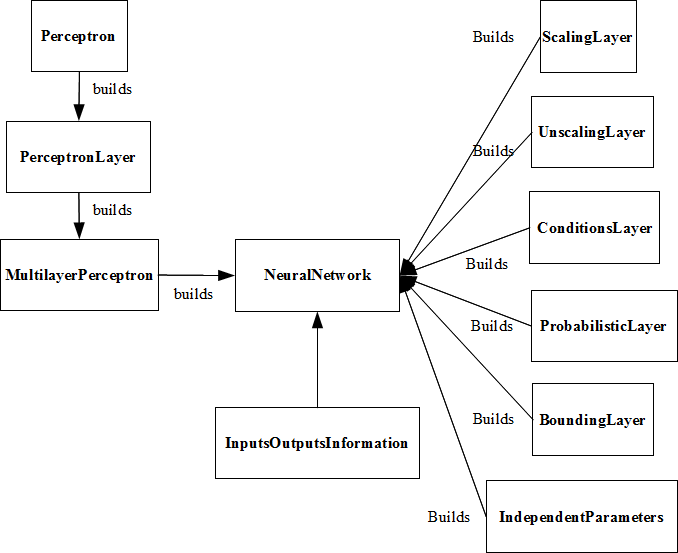
\includegraphics[width=1.1\textwidth]{neural_network/association_diagram}
\caption{Association diagram for the \lstinline'NeuralNetwork' class.}\label{NeuralNetworkAssociationDiagram}
\end{center}
\end{figure}

\subsection*{Derived classes}

The next task is then to establish which classes are abstract and
to derive the necessary concrete classes to be added to the
system. 

The neural network class in \texttt{OpenNN} will be intensively used by any application. 
Therefore, for performance reasons, all the composing classes have been designed to be concrete. 

Let us then examine the classes we have so far:

\begin{description}

\item[Perceptron] The class \lstinline"Perceptron" is concrete,
and can implement different activation functions. 

\item[Perceptron layer] The class \lstinline"PerceptronLayer" is also concrete,
since it is defined as a vector of perceptrons.

\item[Multilayer perceptron] The class \lstinline"MultilayerPerceptron" is a concrete class and is
itself suitable for instantiation. This class is implemented as a vector of layers of perceptrons. 

\item[Scaling layer] The class \lstinline"ScalingLayer" is concrete, and implements the minimum-maximum and mean-standard deviation scaling methods.

\item[Unscaling layer] The class \lstinline"UnscalingLayer" is also concrete, and implements the minimum-maximum and mean-standard deviation unscaling methods.

\item[Bounding layer] The class \lstinline"BoundingLayer" is concrete. It sets to their bound values those inputs which are below or above them. 

\item[Probabilistic layer] The class \lstinline"ProbabilisticLayer" is concrete, and implements the competitive and softmax methods.

\item[Conditions layer] The class \lstinline"ConditionsLayer" has also been designed to be concrete. It implements methods to hold one or two condions. For more difficult situations, further classes must be derived. 

\item[Inputs-outputs information] The class \lstinline"InputsOutputsInformation" is concrete. It mainly stores a few strings with the names, units and descriptions of the neural network variables. 

\item[Independent parameters] The class \lstinline"IndependentParameters" is concrete. It contains other adjustable parameters 
than those belonging to the multilayer perceptron. 

\end{description}

\subsection*{Attributes and operations}

An attribute is a named value or relationship that exists for all
or some instances of a class. An operation is a procedure
associated with a class \cite{Stroustrup2000}. 

In UML class
diagrams, classes are depicted as boxes with three sections: the
top one indicates the name of the class, the one in the middle
lists the attributes of the class, and the bottom one lists the
operations \cite{Rumbaugh1999}.


\begin{description}

\item[Perceptron] A perceptron neuron model has the following attributes:

\begin{itemize}
\item[-] A bias.
\item[-] A set of synaptic weights.
\item[-] The activation function.
\end{itemize}

It performs the following main operations:

\begin{itemize}
\item[-] Calculate the neuron output for a given input.
\item[-] Calculate the derivatives of the output with respect to the inputs.
\end{itemize}


\item[Perceptron layer] The perceptron layer has the following members:

\begin{itemize}
\item[-] A set of perceptrons.
\end{itemize}
 
It performs the following methods:

\begin{itemize}
\item[-] Calculate the layer output for a given input.
\item[-] Calculate the derivatives of the outputs with respect to the inputs.
\end{itemize}

\item[Multilayer perceptron] A multilayer perceptron has the following attributes:

\begin{itemize}
\item[-] A set of layers of perceptrons.
\end{itemize}

It performs the following main operations:

\begin{itemize}
\item[-] Calculate the output for a given input.
\item[-] Calculate the Jacobian for a given input.
\item[-] Calculate the Hessian form for a given input.
\end{itemize}

\item[Scaling layer] The scaling layer has the following members:

\begin{itemize}
\item[-] The main statistics of the variables.
\item[-] The scaling method.
\end{itemize}

It implements the following main members:

\begin{itemize}
\item[-] Calculate the scaled variables for unscaled variables.
\item[-] Calculate the derivatives of the scaling function.
\end{itemize}

\item[Unscaling layer] The unscaling layer is similar to the scaling layer, 
with the following members:

\begin{itemize}
\item[-] The main statistics of the variables.
\item[-] The unscaling method.
\end{itemize}

It implements the following main members:

\begin{itemize}
\item[-] Calculate the unscaled variables for scaled variables.
\item[-] Calculate the derivatives of the unscaling function.
\end{itemize}

\item[Bounding layer] The bounding layer contains the following attributes:

\begin{itemize}
\item[-] The lower and upper bounds of the variables.
\end{itemize}

It performs the following main operations:

\begin{itemize}
\item[-] Calculate bounded variables for unbounded ones.
\item[-] Calculate the derivatives of the bounding function.
\end{itemize}

\item[Probabilistic layer] The probabilist layer contains:

\begin{itemize}
\item[-] The probabilistic method.
\end{itemize}

It computes the following functions:

\begin{itemize}
\item[-] Calculate probabilistic variables for non-probabilistic ones.
\item[-] Calculate also the derivatives.
\end{itemize}

\item[Conditions layer] The conditions layer contains the following:

\begin{itemize}
\item[-] The conditions values.
\item[-] The conditions method.
\end{itemize}

   
It performs the following:

\begin{itemize}
\item[-] Calculate outputs holding some conditions. 
\item[-] Calculate also the derivatives of that conditioned outputs.
\end{itemize}

\item[Inputs-outputs information] This class stores the following data:

\begin{itemize}
\item[-] The names, units and descriptions of the input and output variables.
\end{itemize}

It performs the following:

\begin{itemize}
\item[-] Write default names for the inputs and the outputs. 
\end{itemize}

\item[Independent parameters] The class representing independent parameters contains the following main members:

\begin{itemize}
\item[-] A set of parameters.
\item[-] Information and statistics on the parameters.
\item[-] Scaling/Unscaling and bounding methods. 
\end{itemize}

The independent parameters class can perform the follwoing operations:

\begin{itemize}
\item[-] Scale and unscale the parameters.
\item[-] Bounding the parameters. 
\end{itemize}

\end{description}





\section{PerformanceFunctional classes}\label{PerformanceFunctionalClasses}
\index{Performance functional class}
\index{Objective functional classes}

\texttt{OpenNN} implements the \lstinline"PerformanceFunctional" concrete class. 
This class manages different objective, regularization and constraints terms in order to construct a 
performance functional suitable for our problem. 

\subsection*{Members}

The \lstinline"PerformanceFunctional" class contains:

\begin{itemize}
\item[-] The type of objective term.
\item[-] The type of regularization term.
\item[-] The type of constraints term.
\item[-] A pointer to an objective performance term.
\item[-] A pointer to a regularization performance term.
\item[-] A pointer to a constraints performance term.
\end{itemize}

All that members are declared as private, and they can only be used with their corresponding get or set methods. 

\subsection*{Constructors}

As it has been said, the choice of the performance functional depends on the particular application. 
A default performance functional is not associated to a neural network, it is not measured on a data set or a mathematical model,

\begin{lstlisting}
PerformanceFunctional pf;
\end{lstlisting}

The default objective functional in the performance functional above is a normalized squared error. 
This is very used in function regression, pattern recognition and time series prediction. 

That performance functional does not contain any regularization or constraints terms by default. Also, it does not have  numerical differentiation utilities. 

The following sentence constructs a performance functional associated to a neural network and to be measured on a data set.

\begin{lstlisting}
NeuralNetwork nn(1, 1);

DataSet ds(1, 1, 1);
ds.initialize_data(0.0);

PerformanceFunctional pf(&nn, &ds);
\end{lstlisting}

As before the default objective functional is the normalized squared error. 

\subsubsection*{Methods}

% Evaluation

The \lstinline"calculate_performance" method calculates the performance of some neural network. 
It is called as follows, 

\begin{lstlisting}
double performance = pf.calculate_performance();
\end{lstlisting}

Note that the evaluation of the performance functional is the sum of the objective, regularization and constraints terms. 

% Gradient

The \lstinline"calculate_gradient" method calculates the partial derivatives of the performance with respect to the neural network parameters. 

\begin{lstlisting}
PerformanceFunctional pf;

Vector<double> gradient = pf.calculate_gradient();
\end{lstlisting}

As before, the gradient of the performance functional is the sum of the objective, the regularization and the constraints gradients. 

Note that, most of the times, an analytical solution for the gradient is achieved.
An example is the normalized squared error. 
On the other hand, some applications might need numerical differentiation. 
An example is the outputs integrals performance term.

% Hessian

Similarly, the Hessian matrix can be computed using the \lstinline"calculate_Hessian" method, 

\begin{lstlisting}
Matrix<double> Hessian = pf.calculate_Hessian();
\end{lstlisting}

The Hessian of the objective functional is also the sum of the objective, regularization and constraints matrices of second derivatives. 

% Objective method

If the user wants another objective functional than the default, he can writte

\begin{lstlisting}
pf.construct_objective_term('MEAN_SQUARED_ERROR');
\end{lstlisting}

The above sets the objective functional to be the mean squared error. 

% Regularization method

The performance functional is not regularized by default. 
To change that, the following can be used

\begin{lstlisting}
pf.construct_regularization_term('NEURAL_PARAMETERS_NORM');
\end{lstlisting}

The above sets the default regularization method to be the multilayer perceptron parameters norm. 
Also, it sets the weight for that regularization term. 

% Constraints method

Finally, the performance functional does not include a constraints term by default. 
The use of constrains might be difficult, so the interested reader is referred to look at the examples included in OpenNN.  

% Numerical differentiation method

%The default method for numerical differentiation is central differences. If you want to use forward differences instead, you %can write

%\begin{lstlisting}
%MockObjectiveFunctional mof;
%mof.set_numerical_differentiation_method
%(ObjectiveFunctional::ForwardDifferences);
%\end{lstlisting}
%
%
%\subsubsection*{Derived classes}
%\index{SumSquaredError class}
%\index{MeanSquaredError class}
%\index{RootMeanSquaredError class}
%\index{NormalizedSquaredError class}
%\index{MinkowskiError class}
%%\index{CrossEntropyError class}
%
%\index{GeodesicProblem class}
%\index{BrachistochroneProblem class}
%\index{CatenaryProblem class}
%\index{IsoperimetricProblem class}
%
%\index{CarProblem example}
%\index{CarProblemNeurocomputing example}
%\index{FedBatchFermenterProblem example}
%\index{AircraftLandingProblem example}
%
%\index{PrecipitateDissolutionModeling example}
%
%\index{MinimumDragProblem example}
%
%\index{DeJongFunction example}
%\index{RosenbrockFunction example}
%\index{RastriginFunction example}
%\index{PlaneCylinder example}
%%\index{WeldedBeam example}
%
%For data modeling problems, such as function regression or pattern
%recognition, \texttt{OpenNN} includes the
%classes \lstinline"SumSquaredError", \lstinline"MeanSquaredError",
%\lstinline"RootMeanSquaredError",
%\lstinline"NormalizedSquaredError" and \lstinline"MinkowskiError". Read Chapters
%\ref{FunctionRegression} and \ref{PatternRecognition} to learn about modeling of data and the use of that classes.
%
%On the other hand, other types of variational problems require
%programming another derived class. As a way of illustration,
%\texttt{OpenNN} includes the examples \lstinline"GeodesicProblem",
%\lstinline"BrachistochroneProblem", \lstinline"CatenaryProblem" and
%\lstinline"IsoperimetricProblem", which are classical problems in
%the calculus of variations.
%
%Examples for optimal control problems included are
%\lstinline"CarProblem",
%\lstinline"CarProblemNeurocomputing",
%\lstinline"FedBatchFermenterProblem" and
%\lstinline"AircraftLandingProblem", see Chapter
%\ref{OptimalControl}.
%
%Regarding inverse problems, \texttt{OpenNN} includes the example
%\lstinline"PrecipitateDissolutionModeling". Read Chapter
%\ref{InverseProblems} to see how this type of problems are
%formulated and how to solve them by means of a neural network.
%
%As an example of optimal shape design, the
%\lstinline"MinimumDragProblem" example is
%included. All these is explained in
%Chapter \ref{OptimalShapeDesign}.
%
%Finally, \texttt{OpenNN} can be used as a software tool for function
%optimization problems. Some examples included are
%\lstinline"DeJongFunction", \lstinline"RosenbrockFunction",
%\lstinline"RastriginFunction", \lstinline"PlaneCylinder" and \lstinline"WeldedBeam". Please
%read Chapter \ref{FunctionOptimization} if you are
%interested on that.

\subsection*{XML formats}


\subsubsection*{Sum squared error}

The XML format of a sum squared error is as follows.

\begin{lstlisting}
<SumSquaredError>
   <Display>boolean</Display>
</SumSquaredError>
\end{lstlisting}

\subsubsection*{Mean squared error}

The XML format of the mean squared error is very similar to that of the sum squared error.

\begin{lstlisting}
<MeanSquaredError>
   <Display>boolean</Display>
</MeanSquaredError>
\end{lstlisting}

\subsubsection*{Root mean squared error}

The XML format of the root mean squared error is very similar to that of the sum squared error.

\begin{lstlisting}
<RootMeanSquaredError>
   <Display>boolean</Display>
</RootMeanSquaredError>
\end{lstlisting}

\subsubsection*{Normalized squared error}

The XML format of the normalized squared error is very similar to that of the sum squared error.

\begin{lstlisting}
<NormalizedSquaredError>
   <Display>boolean</Display>
</NormalizedSquaredError>
\end{lstlisting}

\subsubsection*{Minkowski squared error}

The XML format of the root mean squared error is as follows.

\begin{lstlisting}
<MinkowskiError>
   <MinkowskiParameter>real</MinkowskiParameter>
   <Display>boolean</Display>
</MinkowskiError>
\end{lstlisting}

\subsubsection*{Cross entropy error}

The XML format of the cross entropy error is very similar to that of the sum squared error.

\begin{lstlisting}
<CrossEntropyError>
   <Display>boolean</Display>
</CrossEntropyError>
\end{lstlisting}

\subsubsection*{Neural parameters norm}

The XML format of the neural parameters norm performance term is as follows.

\begin{lstlisting}
<NeuralParametersNorm>
   <NeuralParametersNormWeight>real</NeuralParametersNormWeight>
   <Display>boolean</Display>
</NeuralParametersNorm>
\end{lstlisting}

\subsubsection*{Outputs integrals}

The XML format of the outputs integrals performance term is as follows.

\begin{lstlisting}
<OutputsIntegrals>
   <NumericalIntegration>
   numerical_integration_element
   </NumericalIntegration>
   <OutputsIntegralsWeights>real_vector</OutputsIntegralsWeights>
   <Display>boolean</Display>
</OutputsIntegrals>
\end{lstlisting}

\subsubsection*{Final solutions error}

The XML format of the final solutions error performance term is as follows.

\begin{lstlisting}
<FinalSolutionsError>
   <NumericalDifferentiation>
   numerical_differentiation_element
   </NumericalDifferentiation>
   <TargetFinalSolutions>real_vector</TargetFinalSolutions>
   <FinalSolutionsErrorsWeights>real_vector</FinalSolutionsErrorsWeights>
   <Display>boolean</Display>
</FinalSolutionsError>
\end{lstlisting}

\subsubsection*{Solutions error}

The XML format of the solutions error performance term is as follows.

\begin{lstlisting}
<FinalSolutionsError>
   <NumericalDifferentiation>
   numerical_differentiation_element
   </NumericalDifferentiation>
   <SolutionsErrorMethod>string</SolutionsErrorMethod>
   <SolutionsErrorsWeights>real_vector</SolutionsErrorsWeights>
   <Display>boolean</Display>
</FinalSolutionsError>
\end{lstlisting}

\subsubsection*{Independent parameters error}

The XML format of the independent parameters error performance term is as follows.

\begin{lstlisting}
<IndependentParametersError>
   <NumericalDifferentiation>
   numerical_differentiation_element
   </NumericalDifferentiation>
   <TargetIndependentParameters>real_vector</TargetIndependentParameters>
   <IndependentParametersErrorsWeights>real_vector</IndependentParametersErrorsWeights>
   <Display>boolean</Display>
</IndependentParametersError>
\end{lstlisting}

\subsubsection*{Inverse sum squared error}

The XML format of the independent parameters error performance term is as follows.

\begin{lstlisting}
<InverseSumSquaredError>
   <NumericalDifferentiation>
   numerical_differentiation_element
   </NumericalDifferentiation>
   <Display>boolean</Display>
</InverseSumSquaredError>
\end{lstlisting}

\subsubsection{Performance functional}

The XML format of a complete performance functional object is as follows.

\begin{lstlisting}
<PerformanceFunctional>
   <ObjectiveTermType>string</ObjectiveTermType>
   <RegularizationTermType>string</RegularizationTermType>
   <ConstraintsTermType>string</ConstraintsTermType>
   <ObjectiveTermFlag>boolean</ObjectiveTermFlag>
   <RegularizationTermFlag>boolean</RegularizationTermFlag>
   <ConstraintsTermFlag>boolean</ConstraintsTermFlag>
   <ObjectiveTerm>   
   objective_term_element
   </ObjectiveTerm>   
   <RegularizationTerm>   
   regularization_term_element
   </RegularizationTerm>   
   <ConstraintsTerm>   
   constraints_term_element
   </ConstraintsTerm>   
   <Display>boolean</Display>
</PerformanceFunctional>
\end{lstlisting}



%%%%%%%%%%%%%%%%%%%%%%%%%%%%%%%%%%%%%%%%%%%%%%%%%%%%%%%%%%%%%%%%%%%%%%%%%%%%%%%%%%%%
 
\chapter{Training strategy}\label{TrainingStrategy}
The procedure used to carry out the learning process in a neural network is called the
training strategy. A training strategy might be composed of different training algorithms. 




\section{Basic theory}\label{TrainingStrategyBasicTheory}
As we saw in the previous chapter the performance functional has a performance
function associated. 
The performance function for a neural network can be visualized as a hypersurface,
with the parameters as coordinates, see Figure
\ref{PerformanceFunctionFigure}.

\begin{figure}[h!]
\begin{center}
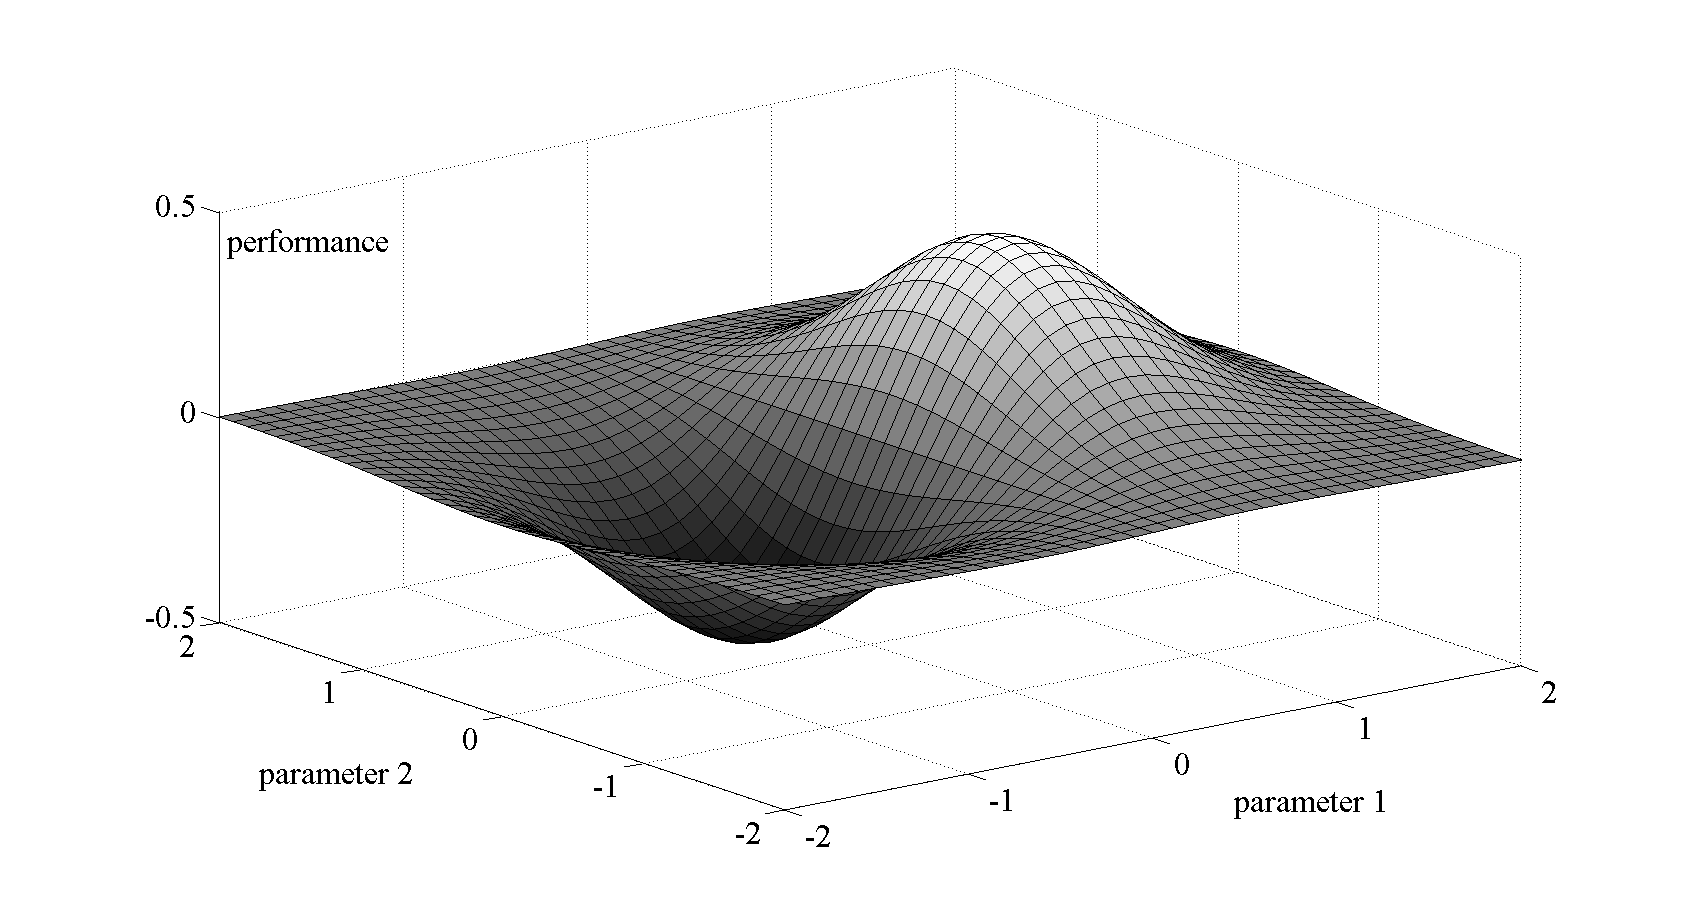
\includegraphics[width=1.0\textwidth]{training_strategy/performance_function.png}
\caption{Geometrical representation of the performance function.}\label{PerformanceFunctionFigure}
\end{center}
\end{figure}

The minimum or maximum value of the performance functional is
achieved for a vector of parameters at which the performance
function takes on a minimum or maximum value. Therefore, the
learning problem for neural networks, formulated as a
variational problem, can be reduced to a function optimization
problem \cite{Lopez2006ICANN}.

In this sense, a variational formulation for neural networks provides a direct method for solving variational 
problems. The universal approximation 
properties for the multilayer perceptron cause neural computation to
be a very appropriate paradigm for the solution of these problems.

\subsubsection{One-dimensional optimization}
\index{one dimensional optimization} 
\index{line search|see{one dimensional optimization}}

\index{relative minimum}
\index{local minimum}

\index{relative maximum}
\index{local maximum}

\index{absolute minimum}
\index{global minimum}

\index{absolute maximum}
\index{global maximum}

\index{first training rate}

Although the performance function is multidimensional, one-dimensional optimization methods are of great importance. 
Indeed, one-dimensional optimization algorithms are very often used inside multidimensional optimization algorithms. 

A function is said to have a relative or local minimum at some point if the function is always greater within some neighbourhood of that point. 
Similarly, a point is called a relative or local maximum if the function is always lesser within some neighbourhood of that point. 

The function is said to have a global or absolute minimum at some point if the function is always greater within the whole domain. 
Similarly, a point will be a global maximum if the function is always greater within the whole domain. 
Finding a global optimum is, in general, a very difficult problem \cite{Wolpert1997}. 

On the other hand, the tasks of maximization and minimization are trivially related to
each other, since maximization of a function is
equivalent to minimization of its negative, and vice
versa.

In this regard, a one-dimensional optimization problem is one in which the argument which minimizes the performance function is to be found. 

The necessary condition states that if the directional performance function has a relative optimum  and if the derivative exists as a finite number. 
The condition for the optimum to be a minimum is that the second derivative is greater than zero, and vice versa. 

The most elementary approach for one-dimensional optimization problems is to use a fixed step size or training rate. 
More sophisticated algorithms which are are widely used are the golden section method and the
Brent's method. Both of the two later algortims begin by bracketing a minimum. 

%\subsubsection{Fixed training rate}
%\index{fixed training rate}
%\index{fixed step size|see fixed training rate}

%The most elementary approach for such a problem is to use a fixed step size, or training rate, and move
%from an initial guess point in a favorable direction (positive or negative). The step size
%used must be small in relation to the final accuracy desired. Although this method is
%very simple to implement, it is not efficient in many cases.

The golden section method brackets that minimum until the distance
between the two outer points in the bracket is less than a defined
tolerance \cite{Press2002}.

The Brent's method performs a parabolic
interpolation until the distance between the two outer points
defining the parabola is less than a tolerance \cite{Press2002}.


\subsubsection{Multi-dimensional optimization}

\index{function optimization problem}
\index{performance function}
\index{global minimum, performance function}
\index{local minimum, performance function}

\index{global minimum condition}
\index{local minimum condition}

\index{epoch}
\index{iteration|see{epoch}}

\index{parameters increment}
\index{training direction}
\index{training rate}

\index{evaluation improvement}

\index{stopping criteria}

\index{minimum parameters increment norm}

\index{evaluation goal}
\index{minimum evaluation improvement}
\index{gradient norm goal}

\index{maximum time}
\index{maximum epochs number}

\index{early stopping}

\index{zero order method}
\index{random search}
\index{evolutionary algorithm}
\index{genetic algorithm|see{evolutionary algorithm}}

\index{first order method}
\index{gradient descent method}
\index{conjugate gradient method}
\index{scaled conjugate gradient}
\index{quasi-Newton method} 

\index{second order method}
\index{Newton's method}
\index{Levenberg-Marquardt algorithm}

As it was shown in Chapter \ref{PerformanceFunctional}, the learning problem for neural networks is reduced 
to the searching for a parameter vector at which the performance function takes
a maximum or a minimum value.

The concepts of relative or local and absolute or global optima for the multidimensional case apply in the same way as for the one-dimensional case. The tasks of maximization and minimization are also trivially related here. 

The necessary condition states that if the neural network is at a minimum of the performance function, 
then the gradient is the zero vector. 

The performance function is, in general, a non linear function of the
parameters. As a consequence, it is not possible to find closed
training algorithms for the minima. Instead, we consider a search
through the parameter space consisting of a succession of steps, or
epochs. 

At each epoch, the performance will increase by adjusting the neural network parameters. 
The change of parameters between two epochs is called the parameters increment. 

In this way, to train a neural network we start with some parameters vector 
(often chosen at random) and we generate a sequence of parameter vectors, so
that the performance function is reduced at each iteration of the algorithm. 
The change of performance between two epochs is called the performance improvement. 

The training algorithm stops when a specified condition is satisfied. 
Some stopping criteria commonly used are \cite{Demuth2009}:

\begin{enumerate}
\item The parameters increment norm is less than a minimum value. 
\item The performance improvement in one epoch is less than a set value.
\item Performance has been minimized to a goal value.
\item The norm of the performance function gradient falls below a goal.
\item A maximum number of epochs is reached.
\item A maximum amount of computing time has been exceeded.
\end{enumerate}

A stopping criterium of different nature is early stopping. 
This method is used in ill-possed problems in order to control the effective complexity of the neural network. 
Early stopping is a very common practice in neural networks and often produces good solutions to ill-possed problems. 

Figure \ref{TrainingProcess} is a state diagram of the training
procedure, showing states and transitions in the training process
of a neural network.

\begin{figure}[h!]
\begin{center}
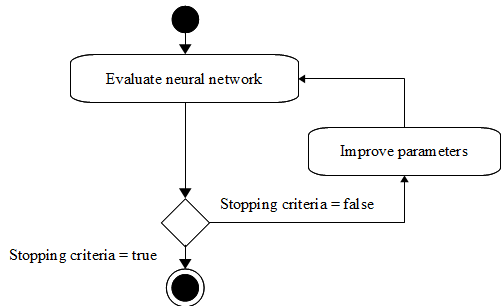
\includegraphics[width=0.8\textwidth]{training_strategy/training_process.png}
\caption{Training process.}\label{TrainingProcess}
\end{center}
\end{figure}

The training process is determined by the way in which the
adjustment of the parameters in the neural network takes place.
There are many different training algorithms, which have a variety
of different computation and storage requirements. Moreover, there
is not a training algorithm best suited to all locations
\cite{Wolpert1997}.

Training algorithms might require information from the performance
function only, the gradient vector of the performance function or the
Hessian matrix of the performance function \cite{Press2002}. These
methods, in turn, can perform either global or local optimization.

Zero-order training algorithms make use of the performance function
only. The most significant zero-order
training algorithms are stochastic, which involve randomness in the
optimization process. Examples of these are random
search and evolutionary
algorithms \cite{Goldberg1988}
\cite{Fogel1994} or particle swarm optimization \cite{Kennedy1995},
which are global optimization methods .

First-order training algorithms use the performance function and its
gradient vector \cite{Battiti1992}.
Examples of these are gradient descent methods, conjugate gradient methods, scaled conjugate gradient methods \cite{Moller1993} or quasi-Newton
methods. Gradient descent, conjugate
gradient, scaled conjugate gradient and quasi-Newton methods are
local optimization methods \cite{Luenberger1984}.

Second-order training algorithms make use of the performance function,
its gradient vector and its Hessian matrix \cite{Battiti1992}. Examples for second-order methods are
Newton's method and the Levenberg-Marquardt
algorithm \cite{Hagan1994}.
Both of them are local optimization methods \cite{Luenberger1984}.

\subsubsection{Training strategy}

Most of the times, application of a single training algorithm is enough to properly train a neural network. 
The quasi-Newton method is in general a good choice, since it provides good training times and deals successfully with most of the performance functions. 
The Levenberg-Marquardt algorithm could be also recommended for small and medium-sized data modelling problems. 
 
However, some applications might need more training effort. 
In that cases we can combine different algorithms in order to do our best. 
In problems defined by mathematical models, with constraints, etc. a single training algorithm might fail. 

Therefore, for difficult problems, we can try two use two or three different training algorithms. 
A general strategy consists on applying three different training algorithms: 

\begin{enumerate}
\item Initialization training algorithm. 
\item Main training algorithm. 
\item Refinement training algorithm. 
\end{enumerate}

The initialization training algorithm is used to bring the neural network to a stable region of the performance function.
Near the optimum, the performance function usually behaves better than far away. 
Zero order training algorithms, such as random search or the evolutionary algorithm might good for this initialization process. 
Indeed, they are very robust algorithms. 

The main training algorithm does most of the job. The training strategy relies on them. 
First order training algorithms, such as the quasi-Newton method are a good choce here. 

Finally, a refinement training algorithm can be used when a big accuracy is required. 
Second orden training algorithms, such as the Newton-method, require the most exact information of the performance function. Therefore they can perform better for refinement. 



\section{Software model}\label{TrainingStrategySoftwareModel}
%\section{Derived classes}\index{derived class, object oriented programming}

As we have seen, the \texttt{OpenNN} neural network is composed by a multilayer perceptron plus some other kinds of layers. 
In this section we study the software model of the \lstinline"NeuralNetwork" class. 


\subsection*{Classes}

The characterization in classes of the concepts studied in the previous section is as follows:

\begin{description}

\item[Perceptron] The class which represents the concept of perceptron neuron model is called \lstinline"Perceptron".

\item[PerceptronLayer] The class representing a layer of perceptrons is called \lstinline"PerceptronLayer".

\item[MultilayerPerceptron] The class which represents a feed-forward architecture of perceptron layers is called \lstinline"MultilayerPerceptron".

\item[Scaling layer] The class which represents a layer for scaling variables is called \lstinline"ScalingLayer".

\item[Unscaling layer] The class which represents an unscaling layer is called \lstinline"UnscalingLayer".
 
\item[Bounding layer] The class representing a layer of bounding neurons is called \lstinline"BoundingLayer".

\item[Conditions layer] The class wich applies input-output conditions is called \lstinline"ConditionsLayer".

\item[Independent parameters] A class containing parameters not belonging to the multilayer perceptron is called \lstinline"IndependentParameters".

\item[Neural network] The class which aggregates all the different neural network concepts is called \lstinline"NeuralNetwork".

\end{description}

\subsection*{Associations}

The appropriate associations between all the neural networks classes in the system are next identified to be included
to the association diagram:

\begin{description}

\item[Perceptron layer - perceptron] A layer of perceptrons is composed of perceptrons.

\item[Multilayer perceptron - perceptron layer] A multilayer perceptron is composed of layers of perceptrons.

\item[Neural network - Multilayer perceptron] A neural network very probably contains a multilayer perceptron.

\item[Neural network - Scaling layer] A multilayer perceptron usually contains a scaling layer. 

\item[Neural network - Unscaling layer] A multilayer perceptron usually contains an unscaling layer. 

\item[Neural network - Bounding layer] A multilayer perceptron sometimes contains a bounding layer.

\item[Neural network - Probabilistic layer] A multilayer perceptron sometimes contains a probabilistic layer.

\item[Neural network - Conditions layer] A multilayer perceptron might contain a conditions layer.

\item[Neural network - Independent parameters] A multilayer percetpron might contain a set of independent parameters.    

\end{description}

Figure \ref{NeuralNetworkAssociationDiagram} depicts an association diagram
for the neural network class. 

\begin{figure}[h!]
\begin{center}
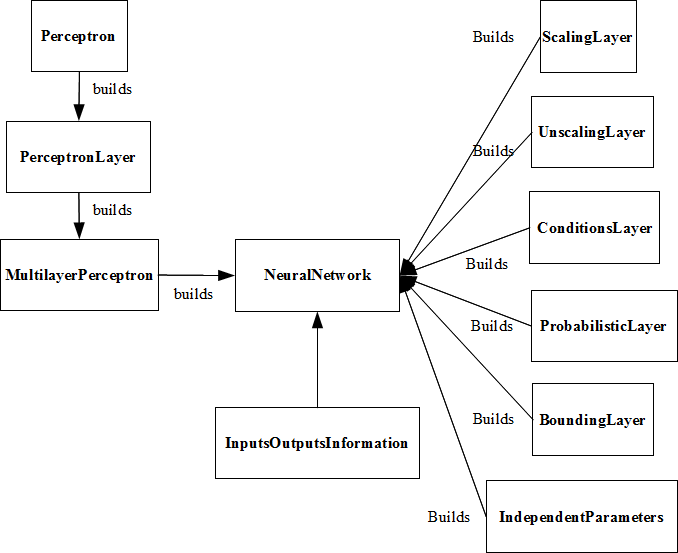
\includegraphics[width=1.1\textwidth]{neural_network/association_diagram}
\caption{Association diagram for the \lstinline'NeuralNetwork' class.}\label{NeuralNetworkAssociationDiagram}
\end{center}
\end{figure}

\subsection*{Derived classes}

The next task is then to establish which classes are abstract and
to derive the necessary concrete classes to be added to the
system. 

The neural network class in \texttt{OpenNN} will be intensively used by any application. 
Therefore, for performance reasons, all the composing classes have been designed to be concrete. 

Let us then examine the classes we have so far:

\begin{description}

\item[Perceptron] The class \lstinline"Perceptron" is concrete,
and can implement different activation functions. 

\item[Perceptron layer] The class \lstinline"PerceptronLayer" is also concrete,
since it is defined as a vector of perceptrons.

\item[Multilayer perceptron] The class \lstinline"MultilayerPerceptron" is a concrete class and is
itself suitable for instantiation. This class is implemented as a vector of layers of perceptrons. 

\item[Scaling layer] The class \lstinline"ScalingLayer" is concrete, and implements the minimum-maximum and mean-standard deviation scaling methods.

\item[Unscaling layer] The class \lstinline"UnscalingLayer" is also concrete, and implements the minimum-maximum and mean-standard deviation unscaling methods.

\item[Bounding layer] The class \lstinline"BoundingLayer" is concrete. It sets to their bound values those inputs which are below or above them. 

\item[Probabilistic layer] The class \lstinline"ProbabilisticLayer" is concrete, and implements the competitive and softmax methods.

\item[Conditions layer] The class \lstinline"ConditionsLayer" has also been designed to be concrete. It implements methods to hold one or two condions. For more difficult situations, further classes must be derived. 

\item[Inputs-outputs information] The class \lstinline"InputsOutputsInformation" is concrete. It mainly stores a few strings with the names, units and descriptions of the neural network variables. 

\item[Independent parameters] The class \lstinline"IndependentParameters" is concrete. It contains other adjustable parameters 
than those belonging to the multilayer perceptron. 

\end{description}

\subsection*{Attributes and operations}

An attribute is a named value or relationship that exists for all
or some instances of a class. An operation is a procedure
associated with a class \cite{Stroustrup2000}. 

In UML class
diagrams, classes are depicted as boxes with three sections: the
top one indicates the name of the class, the one in the middle
lists the attributes of the class, and the bottom one lists the
operations \cite{Rumbaugh1999}.


\begin{description}

\item[Perceptron] A perceptron neuron model has the following attributes:

\begin{itemize}
\item[-] A bias.
\item[-] A set of synaptic weights.
\item[-] The activation function.
\end{itemize}

It performs the following main operations:

\begin{itemize}
\item[-] Calculate the neuron output for a given input.
\item[-] Calculate the derivatives of the output with respect to the inputs.
\end{itemize}


\item[Perceptron layer] The perceptron layer has the following members:

\begin{itemize}
\item[-] A set of perceptrons.
\end{itemize}
 
It performs the following methods:

\begin{itemize}
\item[-] Calculate the layer output for a given input.
\item[-] Calculate the derivatives of the outputs with respect to the inputs.
\end{itemize}

\item[Multilayer perceptron] A multilayer perceptron has the following attributes:

\begin{itemize}
\item[-] A set of layers of perceptrons.
\end{itemize}

It performs the following main operations:

\begin{itemize}
\item[-] Calculate the output for a given input.
\item[-] Calculate the Jacobian for a given input.
\item[-] Calculate the Hessian form for a given input.
\end{itemize}

\item[Scaling layer] The scaling layer has the following members:

\begin{itemize}
\item[-] The main statistics of the variables.
\item[-] The scaling method.
\end{itemize}

It implements the following main members:

\begin{itemize}
\item[-] Calculate the scaled variables for unscaled variables.
\item[-] Calculate the derivatives of the scaling function.
\end{itemize}

\item[Unscaling layer] The unscaling layer is similar to the scaling layer, 
with the following members:

\begin{itemize}
\item[-] The main statistics of the variables.
\item[-] The unscaling method.
\end{itemize}

It implements the following main members:

\begin{itemize}
\item[-] Calculate the unscaled variables for scaled variables.
\item[-] Calculate the derivatives of the unscaling function.
\end{itemize}

\item[Bounding layer] The bounding layer contains the following attributes:

\begin{itemize}
\item[-] The lower and upper bounds of the variables.
\end{itemize}

It performs the following main operations:

\begin{itemize}
\item[-] Calculate bounded variables for unbounded ones.
\item[-] Calculate the derivatives of the bounding function.
\end{itemize}

\item[Probabilistic layer] The probabilist layer contains:

\begin{itemize}
\item[-] The probabilistic method.
\end{itemize}

It computes the following functions:

\begin{itemize}
\item[-] Calculate probabilistic variables for non-probabilistic ones.
\item[-] Calculate also the derivatives.
\end{itemize}

\item[Conditions layer] The conditions layer contains the following:

\begin{itemize}
\item[-] The conditions values.
\item[-] The conditions method.
\end{itemize}

   
It performs the following:

\begin{itemize}
\item[-] Calculate outputs holding some conditions. 
\item[-] Calculate also the derivatives of that conditioned outputs.
\end{itemize}

\item[Inputs-outputs information] This class stores the following data:

\begin{itemize}
\item[-] The names, units and descriptions of the input and output variables.
\end{itemize}

It performs the following:

\begin{itemize}
\item[-] Write default names for the inputs and the outputs. 
\end{itemize}

\item[Independent parameters] The class representing independent parameters contains the following main members:

\begin{itemize}
\item[-] A set of parameters.
\item[-] Information and statistics on the parameters.
\item[-] Scaling/Unscaling and bounding methods. 
\end{itemize}

The independent parameters class can perform the follwoing operations:

\begin{itemize}
\item[-] Scale and unscale the parameters.
\item[-] Bounding the parameters. 
\end{itemize}

\end{description}





\section{TrainingStrategy classes}\label{TrainingStrategyClasses}
\texttt{OpenNN} includes the class \lstinline"TrainingStrategy" to represent the concept of training strategy. 

\subsection*{Members}

The training strategy class contains:

\begin{itemize}
\item[-] A pointer to a performance functional object.
\item[-] A pointer to an initialization training algorithm.
\item[-] A pointer to a main training algorithm.
\item[-] A pointer to a refinement training algorithm.
\item[-] The type of initialization training algorithm.
\item[-] The type of main training algorithm.
\item[-] The type of refinement training algorithm.
\item[-] A flag for using the initialization training algorithm.
\item[-] A flag for using the main training algorithm.
\item[-] A flag for using the refinement training algorithm.
\end{itemize}

All members are private, and must be accessed or modified by means of get and set methods, respectively. 

\subsection*{Constructors}

To construct a training strategy object associated to a performance functional object we do the following:

\begin{lstlisting}
TrainingStrategy ts(&pf);
\end{lstlisting}

\noindent where \lstinline"pf" is some performance functional object. 

\subsection*{Methods}

The default training strategy consists on a main training algorithm of the quasi-Newton method type. 
The next sentence sets a different training strategy.

\begin{lstlisting}
RandomSearch* rsp = new RandomSearch(&pf);
rsp->set_epochs_number(10);
ts.set_initialization_training_algorithm(rsp);


GradientDescent* gdp = new GradientDescent(&pf);
gdp->set_epochs_number(25);
ts.set_main_training_algorithm(gdp);
\end{lstlisting}


The most important method of a training strategy is called \lstinline"perform_training". 
The use is as follows:

\begin{lstlisting}
ts.perform_training();
\end{lstlisting}

\noindent where \lstinline"ts" is some training strategy object. 

We can save the above object to a XML file. 

\begin{lstlisting}
ts.save("training_strategy.xml");
\end{lstlisting}


\subsection*{XML formats}

In this section we list the XML formats of the training strategy classes in \texttt{OpenNN}. 

\subsubsection*{Training rate algorithm}

Some training algorithms contain a training rate object inside. 
The format of this object is listed below. 

\begin{lstlisting}
<TrainingRateAlgorithm>
   <TrainingRateMethod>string</TrainingRateMethod>
   <BracketingFactor>real</BracketingFactor>
   <FirstTrainingRate>real</FirstTrainingRate>
   <Display>boolean</Display>
</TrainingRateAlgorithm> 
\end{lstlisting}

\subsubsection*{Gradient descent}
   
The file format of this class is listed below. 

\begin{lstlisting}
<GradientDescent>
   <TrainingRate>
   training_rate_element
   </TrainingRate>
   <WarningTrainingRate>real</WarningTrainingRate>
   <ErrorTrainingRate>real<ErrorTrainingRate>
   
   <MinimumParametersIncrementNorm>real</MinimumParametersIncrementNorm>
   <EvaluationGoal>real</EvaluationGoal>
   <MinimumEvaluationImprovement>real</MinimumEvaluationImprovement>
   <GradientNormGoal>real</GradientNormGoal>
   <MaximumEpochsNumber>integer</MaximumEpochsNumber>
   <MaximumTime>real</MaximumTime>
   
   <ReserveElapsedTimeHistory>boolean</ReserveElapsedTimeHistory>
   <ReserveParametersHistory>boolean</ReserveParametersHistory>
   <ReserveParametersNormHistory>boolean</ReserveParametersNormHistory>
   <ReservePerformanceHistory>boolean</ReserveEvaluationHistory>
   <ReserveValidationErrorHistory>boolean</ReserveValidationErrorHistory>
   <ReserveGradientHistory>boolean</ReserveGradientHistory>
   <ReserveGradientNormHistory>boolean</ReserveGradientNormHistory>
   <ReserveTrainingDirectionHistory>boolean</ReserveTrainingDirectionHistory>
   <ReserveTrainingDirectionNormHistory>boolean</ReserveTrainingDirectionNormHistory>
   <ReserveTrainingRateHistory>boolean</ReserveTrainingRateHistory>
   
   <WarningParametersNorm>real</WarningParametersNorm>
   <WarningGradientNorm>real</WarningGradientNorm>
   <Display>boolean</Display>
   <DisplayPeriod>integer</DisplayPeriod>
</GradientDescent>   
\end{lstlisting}

\subsubsection*{Newton method}

The file format of this class is listed below. 

\begin{lstlisting}
<NewtonMethod>
   <TrainingRateMethod>
   training_rate_method
   </TrainingRateMethod>
         
   <WarningParametersNorm>real</WarningParametersNorm>
   <WarningGradientNorm>real</WarningGradientNorm>
   <WarningTrainingRate>real</WarningTrainingRate>
   
   <ErrorParametersNorm>real</ErrorParametersNorm>
   <ErrorGradientNorm>real</ErrorGradientNorm>
   <ErrorTrainingRate>real</ErrorTrainingRate>
   
   <MinimumParametersIncrementNorm>real</MinimumParametersIncrementNorm>
 
   <MinimumEvaluationImprovement>real</MinimumEvaluationImprovement>
   <EvaluationGoal>real</EvaluationGoal>
 
   <GradientNormGoal>real</GradientNormGoal>
   
   <MaximumEpochsNumber>integer</MaximumEpochsNumber>
   
   <MaximumTime>real</MaximumTime>
   
   <ReserveParametersHistory>boolean</ReserveParametersHistory>   
   <ReserveParametersNormHistory>boolean</ReserveParametersNormHistory>

   <ReserveEvaluationHistory>boolean</ReserveEvaluationHistory>   
   <ReserveGeneralizationErrorHistory>boolean</ReserveGeneralizationErrorHistory>
   <ReserveGradientHistory>boolean</ReserveGradientHistory>
   <ReserveGradientNormHistory>boolean</ReserveGradientNormHistory>
   <ReserveInverseHessianHistory>boolean</ReserveInverseHessianHistory>
   
   <ReserveTrainingDirectionHistory>boolean</ReserveTrainingDirectionHistory>
   <ReserveTrainingDirectionNormHistory>boolean</ReserveTrainingDirectionNormHistory>
   <ReserveTrainingRateHistory>boolean</ReserveTrainingRateHistory>
   <ReserveElapsedTimeHistory>boolean</ReserveElapsedTimeHistory>
   
   <Display>boolean</Display>
   <DisplayPeriod>integer</DisplayPeriod>
</NewtonMethod>
\end{lstlisting}


\subsubsection*{Conjugate gradient}

The file format of the conjugate gradien object is as follows:

\begin{lstlisting}
<ConjugateGradient>
   <TrainingDirectionMethod>string</TrainingDirectionMethod>
   
   <TrainingRateAlgorithm>
   training_rate_algorithm_element
   </TrainingRateAlgorithm>
      
   <WarningParametersNorm>real</WarningParametersNorm>
   <WarningGradientNorm>real</WarningGradientNorm>
   <WarningTrainingRate>real</WarningTrainingRate>
   
   <ErrorParametersNorm>real</ErrorParametersNorm>
   <ErrorGradientNorm>real</ErrorGradientNorm>
   <ErrorTrainingRate>real</ErrorTrainingRate>
   
   <MinimumParametersIncrementNorm>real</MinimumParametersIncrementNorm>
  
   <MinimumEvaluationImprovement>real</MinimumEvaluationImprovement> 
   <EvaluationGoal>real</EvaluationGoal>
   <GradientNormGoal>real</GradientNormGoal>
   
   <MaximumEpochsNumber>integer</MaximumEpochsNumber>
   <MaximumTime>real</MaximumTime>
   
   <ReserveParametersHistory>boolean</ReserveParametersHistory>
   <ReserveParametersNormHistory>boolean</ReserveParametersNormHistory>
   
   <ReserveEvaluationHistory>boolean</ReserveEvaluationHistory>
   <ReserveGeneralizationEvaluationHistory>boolean</ReserveGeneralizationEvaluationHistory>
   <ReserveGradientHistory>boolean</ReserveGradientHistory>
   <ReserveGradientNormHistory>boolean</ReserveGradientNormHistory>
   
   <ReserveTrainingDirectionHistory>boolean</ReserveTrainingDirectionHistory>
   <ReserveTrainingDirectionNormHistory>boolean</ReserveTrainingDirectionNormHistory>
   <ReserveTrainingRateHistory>boolean</ReserveTrainingRateHistory>
   <ReserveElapsedTimeHistory>boolean</ReserveElapsedTimeHistory>
   
   <DisplayPeriod>integer</DisplayPeriod>
   <Display>boolean</Display>
</ConjugateGradient>
\end{lstlisting}


\subsubsection*{Quasi-Newton method XML format}

See below for the format of a quasi-Newton method XML-type file in \texttt{OpenNN}.

\begin{lstlisting}
<QuasiNewtonMethod version="3.0">

   <TrainingRateAlgorithm>
   training_rate_algorithm_element
   </TrainingRateAlgorithm>
   
   <WarningParametersNorm>real</WarningParametersNorm>
   <WarningGradientNorm>real</WarningGradientNorm>
   <WarningTrainingRate>real</WarningTrainingRate>
   
   <ErrorParametersNorm>real</ErrorParametersNorm>
   <ErrorGradientNorm>real</ErrorGradientNorm>   
   <ErrorTrainingRate>real</ErrorTrainingRate>
   
   <MinimumParametersIncrementNorm>real</MinimumParametersIncrementNorm>
   
   <MinimumEvaluationImprovement>real</MinimumEvaluationImprovement>
   <EvaluationGoal>real</EvaluationGoal>
   <GradientNormGoal>real</GradientNormGoal>
   
   <MaximumEpochsNumber>integer</MaximumEpochsNumber>
   <MaximumTime>real</MaximumTime>
   
   <ReserveParametersHistory>boolean</ReserveParametersHistory>
   <ReserveParametersNormHistory>boolean</ReserveParametersNormHistory>
   
   <ReserveEvaluationHistory>boolean</ReserveEvaluationHistory>
   <ReserveGeneralizationEvaluationHistory>boolean</ReserveGeneralizationEvaluationHistory>
   <ReserveGradientHistory>boolean</ReserveGradientHistory>   
   <ReserveGradientNormHistory>boolean</ReserveGradientNormHistory>
   <ReserveInverseHessianHistory>boolean</ReserveInverseHessianHistory>
   
   <ReserveTrainingDirectionHistory>boolean</ReserveTrainingDirectionHistory>
   <ReserveTrainingDirectionNormHistory>boolean</ReserveTrainingDirectionNormHistory>
   <ReserveTrainingRateHistory>boolean</ReserveTrainingRateHistory>
   <ReserveElapsedTimeHistory>boolean</ReserveElapsedTimeHistory>
   
   <Display>boolean</Display>
   
   <DisplayPeriod>integer</DisplayPeriod>
</QuasiNewtonMethod>
\end{lstlisting}

\subsubsection*{Levenberg Marquardt algorithm}

The file format of this class is listed below. 

\begin{lstlisting}
<LevenbergMarquardtAlgorithm>
   <LinearAlgebraicEquations>
   linear_algebraic_equations_element
   </LinearAlgebraicEquations>
   <DampingParameter>real</DampingParameter>
   <MinimumDampingParameter>real</MinimumDampingParameter>
   <MaximumDampingParameter>real</MaximumDampingParameter>
   <DampingParameterFactor>real</DampingParameterFactor>

   <WarningParametersNorm>real</WarningParametersNorm>
   <WarningGradientNorm>real</WarningGradientNorm>

   <ErrorParametersNorm>real</ErrorParametersNorm>
   <ErrorGradientNorm>real</ErrorGradientNorm>
 
   <MinimumParametersIncrementNorm>real</MinimumParametersIncrementNorm>
   <EvaluationGoal>real</EvaluationGoal>
   <MinimumEvaluationImprovement>real</MinimumEvaluationImprovement>
   <GradientNormGoal>real</GradientNormGoal>
   <MaximumEpochsNumber>integer</MaximumEpochsNumber>
   <MaximumTime>real</MaximumTime>
   
   <ReserveParametersHistory>boolean</ReserveParametersHistory>
   <ReserveParametersNormHistory>boolean</ReserveParametersNormHistory>

   <ReserveEvaluationHistory>boolean</ReserveEvaluationHistory>
   <ReserveGeneralizationEvaluationHistory>boolean</ReserveGeneralizationEvaluationHistory>
   <ReserveGradientHistory>boolean</ReserveGradientHistory>
   <ReserveGradientNormHistory>boolean</ReserveGradientNormHistory>
   
   <ReserveTrainingDirectionHistory>boolean</ReserveTrainingDirectionHistory>
   <ReserveTrainingDirectionNormHistory>boolean</ReserveTrainingDirectionNormHistory>
   <ReserveTrainingRateHistory>boolean</ReserveTrainingRateHistory>
   <ReserveElapsedTimeHistory>boolean</ReserveElapsedTimeHistory>
   
   <WarningGradientNorm>real</WarningGradientNorm>
   <Display>boolean</Display>
   <DisplayPeriod>integer</DisplayPeriod>
</LevenbergMarquardtAlgorithm>   
\end{lstlisting}

\subsubsection*{Random search}

The file format of this class is listed below. 

\begin{lstlisting}
<RandomSearch>

   <FirstTrainingRate>double</FirstTrainingRate>
   <TrainingRateReductionFactor>double</TrainingRateReductionFactor>
   <TrainingRateReductionPeriod>unsigned int</TrainingRateReductionPeriod>
   <WarningParametersNorm>double</WarningParametersNorm>
   <WarningTrainingRate>double</WarningTrainingRate>
   <ErrorParametersNorm>double</ErrorParametersNorm>
   <ErrorTrainingRate>double</ErrorTrainingRate>
   
   <MinimumParametersIncrementNorm>double</MinimumParametersIncrementNorm>
   <MinimumPerformanceIncrease>double</MinimumPerformanceIncrease>
   <PerformanceGoal>double</PerformanceGoal>
   <MaximumGeneralizationEvaluationDecreases>unsigned int</MaximumGeneralizationEvaluationDecreases>
   <MaximumEpochsNumber>unsigned int</MaximumEpochsNumber>
   <MaximumTime>double</MaximumTime>
   
   <ReserveParametersHistory>bool</ReserveParametersHistory>
   <ReserveParametersNormHistory>bool</ReserveParametersNormHistory>
   <ReserveEvaluationHistory>bool</ReserveEvaluationHistory>
   <ReserveGeneralizationEvaluationHistory>bool</ReserveGeneralizationEvaluationHistory>
   <ReserveTrainingDirectionHistory>bool</ReserveTrainingDirectionHistory>
   <ReserveTrainingDirectionNormHistory>bool</ReserveTrainingDirectionNormHistory>
   <ReserveTrainingRateHistory>bool</ReserveTrainingRateHistory>
   <ReserveElapsedTimeHistory>bool</ReserveElapsedTimeHistory>
   
   <DisplayPeriod>unsigned int</DisplayPeriod>
   <Display>bool</Display>
</RandomSearch>

\end{lstlisting}

\subsubsection*{Evolutionary algorithm}

The next listing shows the format of an evolutionary algorithm data file in \texttt{OpenNN}. 
It is of XML-type. 

\begin{lstlisting}
<EvolutionaryAlgorithm>

   Training operators

   <FitnessAssignmentMethod>string</FitnessAssignmentMethod>
   <SelectionMethod>string</SelectionMethod>
   <RecombinationMethod>string</RecombinationMethod>
   <MutationMethod>string</MutationMethod>
      
   Training parameters
   
   <PopulationSize>integer</PopulationSize>
   <Elitism>boolean</Elitism>
   <SelectivePressure>real</SelectivePressure>
   <RecombinationSize>real</RecombinationSize>
   <MutationRate>real</MutationRate>
   <MutationRange>real</MutationRange>
   
   Stopping criteria
   
   <EvaluationGoal>real</EvaluationGoal>
   <MeanEvaluationGoal>real</MeanEvaluationGoal>
   <StandardDeviationEvaluationGoal>real</StandardDeviationEvaluationGoal>
   
   <MaximumGenerationsNumber>real</MaximumGenerationsNumber>
   <MaximumTime>real</MaximumTime>
      
   Training history
   
   <ReservePopulationHistory>boolean</ReservePopulationHistory>
   <ReserveMeanNormHistory>boolean</ReserveMeanNormHistory>
   <ReserveStandardDeviationNormHistory>boolean</ReserveStandardDeviationNormHistory>
   <ReserveBestNormHistory>boolean</ReserveBestNormHistory>
   
   <ReserveMeanEvaluationHistory>boolean</ReserveMeanEvaluationHistory>
   <ReserveStandardDeviationEvaluationHistory>boolean</ReserveStandardDeviationEvaluationHistory>
   <ReserveBestEvaluationHistory>boolean</ReserveBestEvaluationHistory>
      
   <Display>boolean</Display>
   <DisplayPeriod>integer</DisplayPeriod>
   
</EvolutionaryAlgorithm>
\end{lstlisting}


\subsubsection*{Training strategy}

The XML format of a training strategy class is listed below.
It might contain up to three training algorithms. 

\begin{lstlisting}
<TrainingStrategy>

   <InitializationTrainingAlgorithm>
   initialization_training_algorithm_element
   </InitializationTrainingAlgorithm>
   <MainTrainingAlgorithm>
   main_training_algorithm_element
   </MainTrainingAlgorithm>
   <RefinementTrainingAlgorithm>
   refinement_training_algorithm_element
   </RefinementTrainingAlgorithm>

   <InitializationTrainingAlgorithmFlag>boolean</InitializationTrainingAlgorithmFlag>
   <MainTrainingAlgorithmFlag>boolean</MainTrainingAlgorithmFlag>
   <RefinementTrainingAlgorithmFlag>boolean</RefinementTrainingAlgorithmFlag>
       
   <Display>boolean</Display>
</TrainingStrategy>
\end{lstlisting}



%%%%%%%%%%%%%%%%%%%%%%%%%%%%%%%%%%%%%%%%%%%%%%%%%%%%%%%%%%%%%%%%%%%%%%%%%%%%%%%%%%%%

\chapter{Function regression}\label{FunctionRegression}
Many classes included with \texttt{OpenNN} are related to the problem of function regression, since these type of problems are traditional learning tasks for neural networks. The C++ code here include the
data set classes, a number of performance terms, the model selection class and some testing methods for function regression. 



\section{Basic theory}\label{BasicTheoryFunctionRegression}
\index{regression function}
\index{generalization}

\subsection*{Introduction}

Here the neural network learns from knowledge represented by a data set consisting of input-target instances. The targets
are a specification of what the response to the inputs should be, and are represented as continuous variables. 

The basic goal in a function regression problem is to model the
conditional distribution of the target variables, conditioned on
the input variables \cite{Bishop1995}. This function is called the
regression function.

The formulation of a function regression problem requires:

\begin{itemize}
\item[-] A data set. 
\item[-] A neural network.
\item[-] A performance functional.
\item[-] A training strategy.
\item[-] A model selection algorithm.
\item[-] A testing method.
\end{itemize}

A common feature of most data sets is that the data
exhibits an underlying systematic aspect, represented by some
function, but is corrupted with random noise. 

The central goal is to produce a model which exhibits good generalization, or in other words, one which makes good predictions for new data. The best generalization to new data is obtained when the mapping represents the underlying
systematic aspects of the data, rather capturing the specific
details (i.e. the noise contribution) of the particular input-target
set. 

\subsection*{Data set}

\index{data set}
\index{training data set}
\index{generalization data set}
\index{testing data set}

Table \ref{DataSetFunctionRegressionTable} shows the format of a data set for function regression. 
It consists $q$ instances consisting of $n$ input variables and $m$ target variables. 
All input and targets are real values. 

\begin{table}[h!]
\begin{center}
\begin{tabular}{|ccc|ccc|}
\hline
$input_{1,1}$ & $\ldots$ & $input_{1,n}$ & $target_{1,1}$ & $\ldots$ & $target_{1,m}$\\
$input_{2,1}$ & $\ldots$ & $input_{2,n}$ & $target_{2,1}$ & $\ldots$ & $target_{2,m}$\\
$\vdots$ &  & $\vdots$ & $\vdots$ &  & $\vdots$\\ 
$input_{q,1}$ & $\ldots$ & $input_{q,n}$ & $target_{q,1}$ & $\ldots$ & $target_{q,m}$\\
\hline
\end{tabular}\caption{Data set for function regression.}
\label{DataSetFunctionRegressionTable}
\end{center}
\end{table}

When solving function regression problems it is always convenient to split the data set into a training, a generalization and a testing subsets. The size of each subset is up to the designer. Some default values could be to use $60\%$, $20\%$ and $20\%$ of the instances for training, generalization and testing, respectively. 

There are several data splitting methods. Two common approaches are to generate random indices or to specify the required indices for the training, generalization and testing instances.

A simple statistical analysis must be always performed in order to chech for data consistency. Basic statistics of a data set include the mean, standard deviation, minimum and maximum values of input and target variables for the whole data set and the training, generalization and testing subsets. An histogram of each input and target variables should also be plot in order to check the distribution of the available data. 

Also, it is a must to scale the data with the data statistics. 
There are two main data scaling methods, the mean and standard deviation and the minimum and maximum. 

The mean and standard deviation method scales the data for mean $0$ and standard deviation $1$. 
The minimum and maximum method scales the data for minimum $-1$ and maximum $1$. 

\subsection*{Neural network}
\index{neural network}

A neural network is used to represent the regression function. 
The number of inputs must be equal to the number of inputs in the data set, $n$, and the number of outputs must be the number of targets, $m$. 
This neural network will contain a scaling layer, a multilayer perceptron and an unscaling layer. 
It might optionally contain a bounding layer. 
Figure \ref{NeuralNetworkFunctionRegressionFigure} shows a general neural network for solving function regression problems. 

\begin{figure}[h!]
\begin{center}
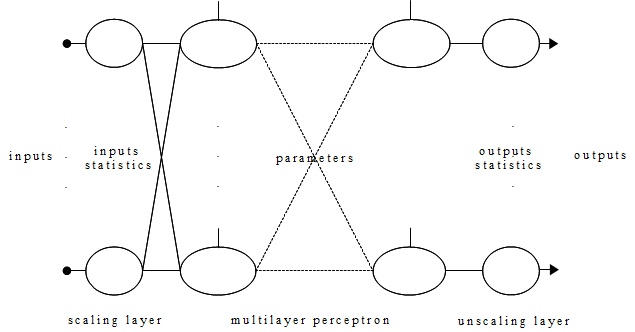
\includegraphics[width=1.2\textwidth]{function_regression/neural_network_function_regression.png}
\caption{Neural network for function regression.}\label{NeuralNetworkFunctionRegressionFigure}
\end{center}
\end{figure}

In general, using a multilayer perceptron with a one hidden layer will be enough. 
A default value to start with for the size of that layer could be 

\begin{eqnarray}\nonumber
\text{hidden neurons number}=\frac{\text{inputs number + outputs number}}{2}. 
\end{eqnarray}

Please note that the complexity which is needed depends very much on the problem at hand, and the above equation is just a rule of thumb. 
However, there are standard methods to find the correct complexity of a neural network for function regression problems. 
The most common is called model selection, which is described later in this section.  

The activation functions for the hidden layers and the output layer are also design variables. 
However, hyperbolic tangent activation function for the hidden layers and linear activation function for the output layer are widely used when solving function regression problems. 

Scaling of inputs and unscaling of outputs should not be used in the design phase, since the data set has been scaled already. When moving to a production phase, the inputs scaling and outputs unscaling methods should be coherent with the scaling method used for the data. 

The neural network in Figure \ref{NeuralNetworkFunctionRegressionFigure} spans a parameterized function space. 
That parameterized space of functions will be the basis to aproximate the regression function. 

\subsection*{Performance functional}
\index{performance functional, function regression}
\index{error functional}

The regression function can be evaluated quantitatively by means of a performance functional of the form

\begin{eqnarray}\nonumber
\text{Performance functional = objective term + regularization term}. 
\end{eqnarray}

For function regression problems, the objective term is measures the error between the outputs from the neural network and the targets in the data set.

In function regression problems, regularization is normally used when the number of instances in the data set 
is small or when the data is noisy. In other situations, regularization might not be necessary.    
  
The solution approach to a function regression problem for is to obtain a neural network which minimizes the performance functional. 
Note that neural networks represent functions. 
In that way, the function regression problem is formulated as a variational problem.


\subsection*{Training strategy}
\index{training algorithm, function regression}

The training strategy is entrusted to solve the reduced function optimization problem by minimizing the performance function. 

In general, evaluation, gradient and Hessian of the error function can be computed analytically. 
Zero order training algorithms, such as the evolutionary algorithm, converge extremely slowly and they are not a good choice. 

On the other hand, second order training algorithms, such as the Newton's method, need evaluation of the Hessian and are neither a good choice. 

In practice, first order algorithms are recommended for solving function regression problems. The Levenberg-Marquardt is a good choice for small and medium sized problems. Due to storage requirements, that algorithm is not recommended for big sized problems, and a quasi-Newton method with BFGS training direction and Brent training rate is preferable. 

In order to study the convergence of the optimization process, it is useful to plot the behaviour of some variables related to the multilayer perceptron, the error functional or the training algorithm as a function of the iteration step. 
Some common training history variables are: 

\begin{itemize}
\item[-] Parameters norm history. 
\item[-] Evaluation history. 
\item[-] Generalization evaluation history. 
\item[-] Gradient norm history. 
\item[-] Training direction norm history. 
\item[-] Training rate history. 
\item[-] Elapsed time history.
\end{itemize}

Form all the training history variables, may be the most important one is the evaluation history. 
Also, it is important to analyze the final values of some variables. 
The most important training results numbers are: 

\begin{itemize}
\item[-] Final parameters. 
\item[-] Final parameters norm. 
\item[-] Final error. 
\item[-] Final generalization error. 
\item[-] Final gradient. 
\item[-] Final gradient norm. 
\item[-] Number of iterations. 
\item[-] Training time. 
\end{itemize}

\subsection*{Model selection}
\index{model selection}

Two frequent problems in function regression are called underfitting and overfitting. 
The best generalization is achieved by using a model whose complexity is the most appropriate to produce an adequate fit of the data \cite{Bishop1995}. 
In this way underfitting is defined as the effect of a generalization error increasing due to a too simple model, 
whereas overfitting is defined as the effect of a generalization error increasing due to a too complex model.

%Figure XXX shows an underfitting case for a function regression problem. 
%In this case we have used a neural network which is too simple to produce an adequate fit. 

%Figure XXX. Underfitting illustration.

%Figure XXX shows an overfitting case for a function regression problem. 
%Here the error on the training data set is very small, but when new data is presented to the neural network the error is large. The neural network has memorized the training examples, but it has not learned to generalize to new situations. 
%The model is too complex to produce an adequate fit.
%Figure XXX. Overfitting illustration.

%Finally, Figure XXX shows a case in which the neural network has a proper complexity to produce a good fit of the data.
%Figure XXX. Good fitting illustration.

While underfitting can be prevented by simply increasing the complexity of the neural network, it is more difficult in advance to prevent overfitting.

A common method for preventing overfitting is to use a regularization term in the performance functional expression. 

However, the best method for avoiding underfitting and overfitting is to use a neural network that is just large enough to provide an adequate fit. 
Such a neural network will not have enough power to overfit the data. 
Unfortunately, it is difficult to know beforehand how large a neural network should be for a specific application.
A technique for that is called model selection. 

In this technique the data set is divided into a training and a generalization subsets. 
The training subset is used for training the neural network by means of the training strategy. 
On the other hand, the error on the generalization subset is monitored during the training process. 
The generalization error normally decreases during the initial phase of training, as it does the training error.

However, when the neural network begins to overfit the data, the error on the generalization subset typically begins to rise. 
When the generalization error increases for a specified number of iterations, the training is stopped, and the parameters at the minimum of the generalization error are set to the neural network.

This process is repeated for several network architectures, and the final training and generalization errors are plotted. 
The optimal network architecture will be that providing minimal generalization error. 
Figure \ref{ModelSelectionFunctionRegression} illustrates this generalization analysis. 

\begin{figure}[h!]
\begin{center}
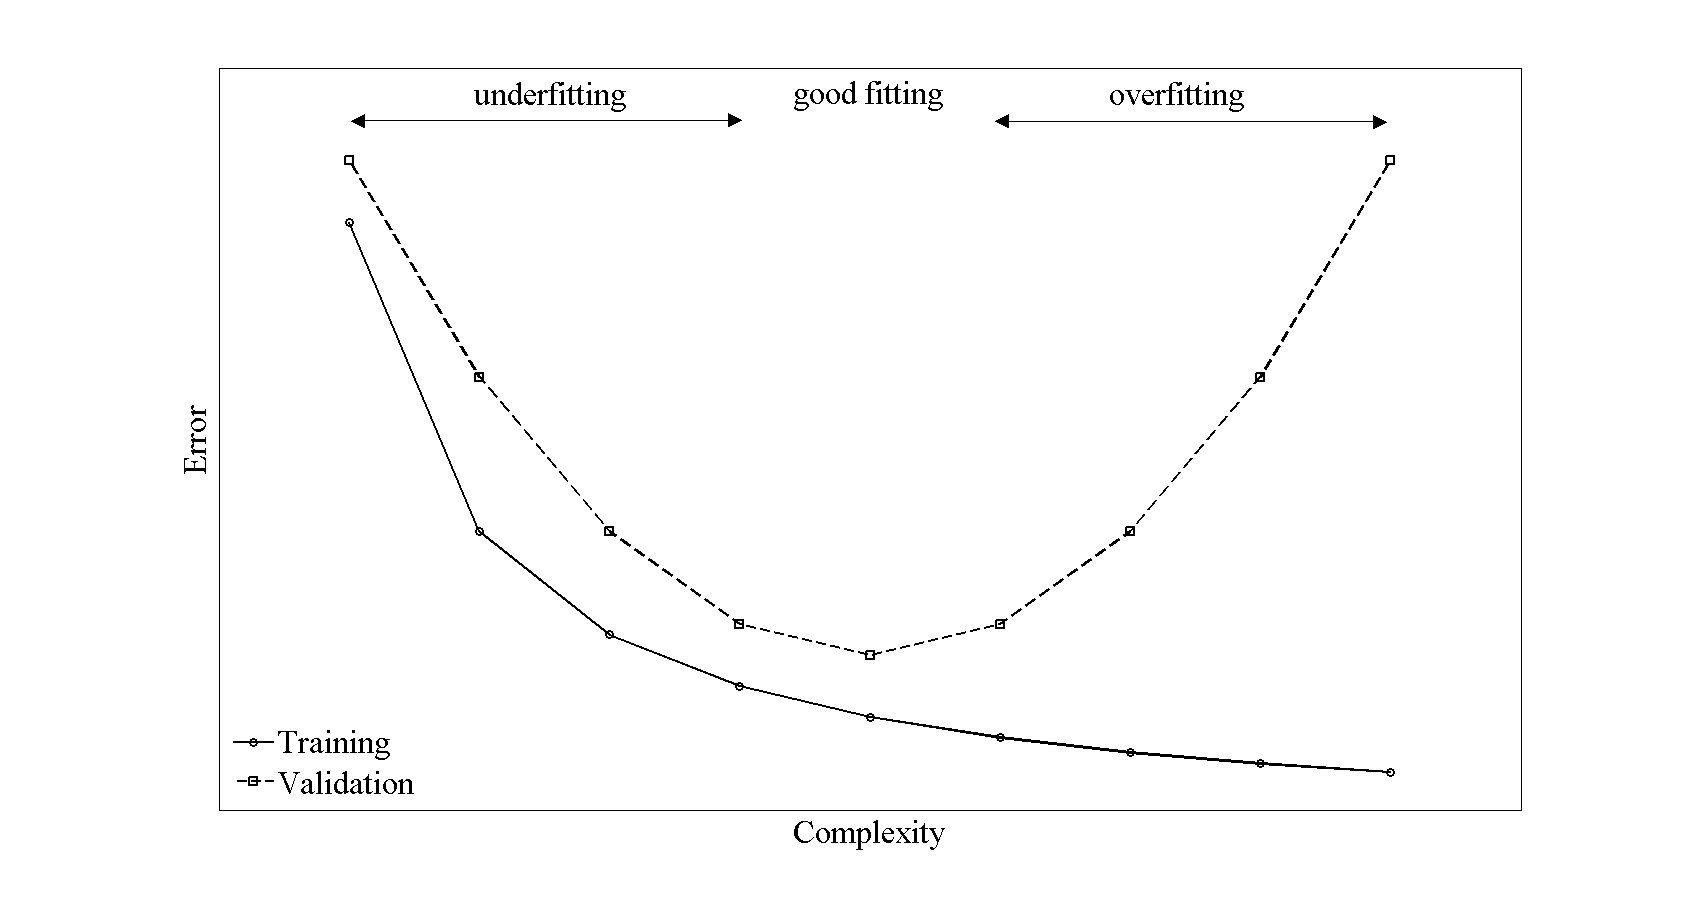
\includegraphics[width=1.0\textwidth]{function_regression/model_selection.png}
\caption{Model selection plot for function regression.}\label{ModelSelectionFunctionRegression}
\end{center}
\end{figure}


\subsection*{Testing analysis}
\index{linear regression analysis}

The performance of a neural network can be measured to some extent
by the performance evaluation on the testing set, but it is useful to
investigate the response in more detail. One option is to perform
a regression analysis between the network response and the
corresponding targets for an independent testing subset.

This analysis leads to $3$ parameters for each output variable. The first two parameters, $a$ and $b$,
correspond to the y-intercept and the slope of the best linear
regression relating outputs and targets. The third parameter, $R^{2}$,  is the correlation coefficient between the outputs and the targets. 

If we had a perfect fit (outputs exactly equal to targets), the slope would be $1$, and the
y-intercept would be $0$. If the correlation coefficient is equal to $1$, then there is perfect correlation between
the outputs from the neural network and the targets in the testing subset. 

Figure \ref{LinearRegressionAnalysis} illustrates a linear regression analysis.  

\begin{figure}[h!]
\begin{center}
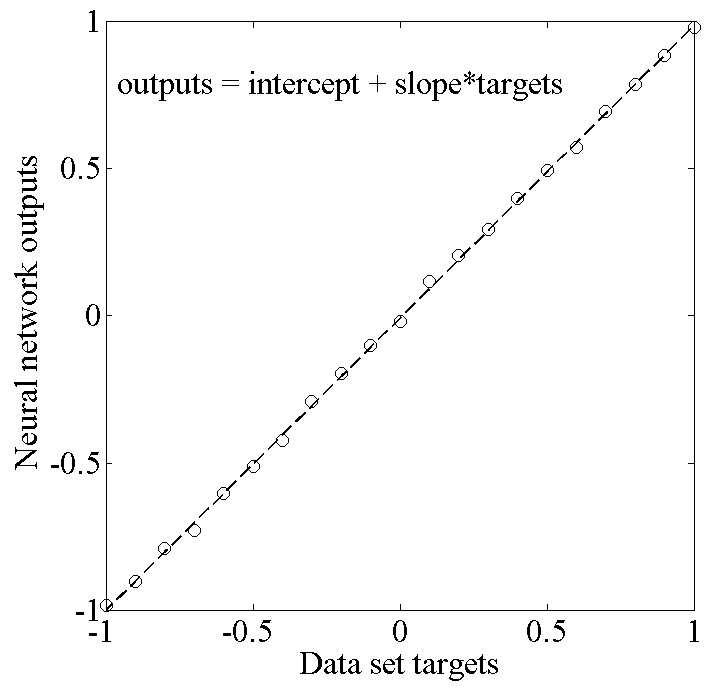
\includegraphics[width=0.6\textwidth]{function_regression/linear_regression_analysis.png}
\caption{Linear regression analysis.}\label{LinearRegressionAnalysis}
\end{center}
\end{figure}


 
\section{Examples}\label{ExamplesFunctionRegression}
\subsection*{Simple function regression}

In this example we have a data set with $1$ input variable, $x$, $1$ target variable, $y$, and $101$ instances. 
The aim is to design a neural network that can predict $y$ values for given $x$ values. 
Figure \ref{SimpleFunctionRegressionDataSet} shows this data set.

\begin{figure}[!hbp]
\begin{center}
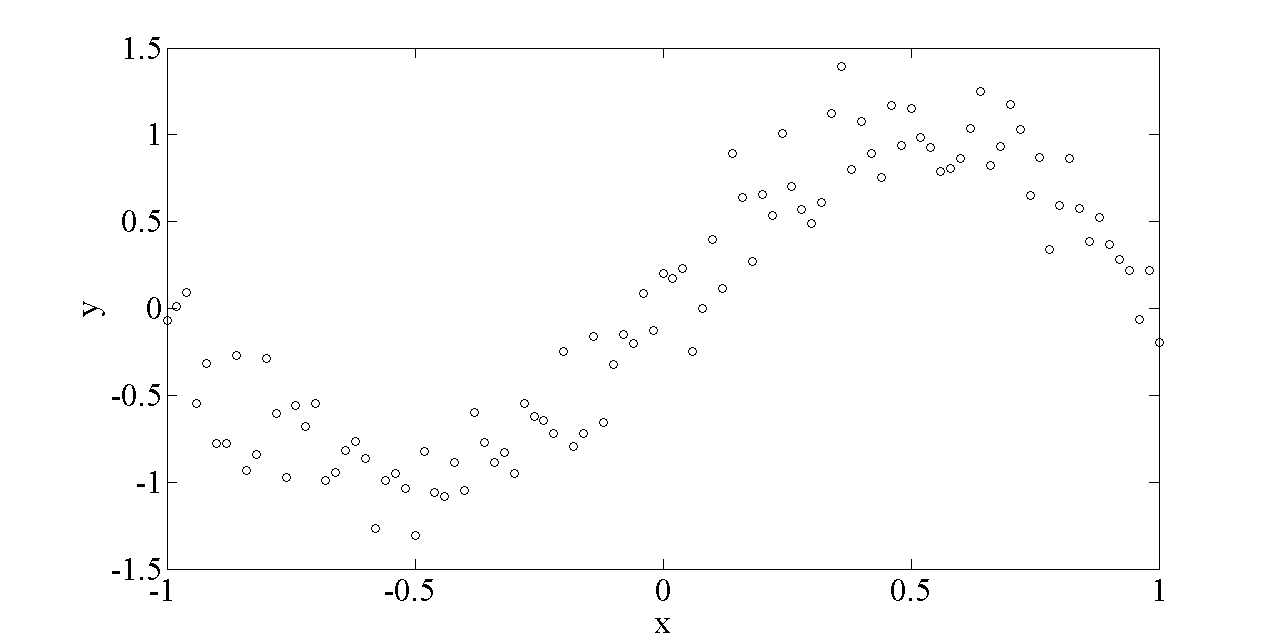
\includegraphics[width=1.0\textwidth]{function_regression/simple_function_regression_data_set.png}
\caption{Simple function regression data set.}\label{SimpleFunctionRegressionDataSet}
\end{center}
\end{figure}

Here the neural network composed of a multilayer perceptron. 
The performance functional is composed of an objective term, the normalized squared error. 
Finally, the training strategy is composed of a main training algorithm, the quasi-Newton method. 

\subsection*{Yacht resistance}

Prediction of residuary resistance of sailing yachts at the
initial design stage is of a great value for evaluating the ship's
performance and for estimating the required propulsive power.
Essential inputs include the basic hull dimensions and the boat
velocity. 
Figure \ref{SailingYatchsFigure} illustrates this example. 
That picture has been taken from Wikipedia. 

\begin{figure}[!hbp]
\begin{center}
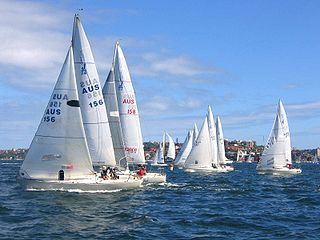
\includegraphics[width=0.7\textwidth]{function_regression/sailing_yatchs.jpg}
\caption{Sailing yatchs.}\label{SailingYatchsFigure}
\end{center}
\end{figure}

The Delft series are a semi-empirical model developed for that
purpose from an extensive collection of full-scale experiments. They
are expressed as a set of polynomials, and provide a prediction of
the residuary resistance per unit weight of displacement, with hull
geometry coefficients as variables and for discrete values of the
Froude number \cite{Gerritsma1981}. The Delft series are widely used
in the sailing yacht industry.

The Delft data set comprises 308 full-scale experiments, which were
performed at the Delft Ship Hydromechanics Laboratory
\cite{Gerritsma1981}. These experiments include 22 different hull
forms, derived from a parent form closely related to the `Standfast
43' designed by Frans Maas. 

As it has been said, variations concern hull geometry coefficients and the
Froude number:

\begin{enumerate}
\item Longitudinal position of the center of buoyancy, adimensional.
\item Prismatic coefficient, adimensional.
\item Length-displacement ratio, adimensional.
\item Beam-draught ratio, adimensional.
\item Length-beam ratio, adimensional.
\item Froude number, adimensional.
\end{enumerate}

Also, the measured variable is the residuary resistance per unit weight of
displacement:

\begin{enumerate}
\item Residuary resistance per unit weight of displacement, adimensional.
\end{enumerate}

In this example, the neural network is composed by a multilayer perceptron with scaling and unscaling layers. 
The performance functional is composed of just an objective term, the normalized squared error. 
Finally, the training strategy is only composed of a main training algorithm, the quasi-Newton method. 

\subsection*{Airfoil noise}

The noise generated by an aircraft is an efficiency and
environmental matter for the aerospace industry. An important component of the total airframe noise is the airfoil
self-noise, which is due to the interaction between an airfoil blade
and the turbulence produce in its own boundary layer and near wake.
Figure \ref{AircraftNoiseFigure} illustrates this example. 
That picture has been taken from Wikipedia. 

\begin{figure}[!hbp]
\begin{center}
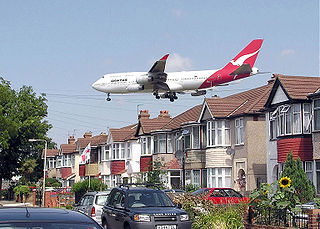
\includegraphics[width=0.7\textwidth]{function_regression/aircraft_noise.jpg}
\caption{Aircraft noise.}\label{AircraftNoiseFigure}
\end{center}
\end{figure}

The self-noise data set used in this example was processed by NASA in
1989 \cite{Brooks1989}, and so it is referred here to as the NASA
data set. It was obtained from a series of aerodynamic and acoustic
tests of two and three-dimensional airfoil blade sections conducted
in an anechoic wind tunnel. 

The NASA data set comprises different size NACA 0012 airfoils at
various wind tunnel speeds and angles of attack. The span of the
airfoil and the observer position were the same in all of the
experiments. The NASA data set contains $1503$ instances. 

In that way, this problem has the following inputs:

\begin{enumerate}
\item Frequency, in Hertzs.
\item Angle of attack, in degrees.
\item Chord length, in meters.
\item Free-stream velocity, in meters per second.
\item Suction side displacement thickness, in meters.
\item Scaled sound pressure level, in decibels.
\end{enumerate}

The only output is:

\begin{enumerate}
\item Scaled sound pressure level, in decibels.
\end{enumerate}

In this example, the neural network is composed by a multilayer perceptron with scaling and unscaling layers. 
The performance functional is composed of just an objective term, the normalized squared error. 
Finally, the training strategy is only composed of a main training algorithm, the quasi-Newton method. 



%%%%%%%%%%%%%%%%%%%%%%%%%%%%%%%%%%%%%%%%%%%%%%%%%%%%%%%%%%%%%%%%%%%%%%%%%%%%%%%%%%%%
 
\chapter{Pattern recognition}\label{PatternRecognition}
Pattern recognition is also a traditional learning task for neural networks. 
\texttt{OpenNN} classes which are related to the solution of pattern recognition problems include the data set, 
several performance terms, the model selection and the testing analysis classes. 



\section{Basic theory}\label{PatternRecognitionBasicTheory}
\index{data set}
\index{nominal variables}
\index{multilayer perceptron}
\index{performance functional, pattern recognition}
\index{training algorithm, pattern recognition}
\index{underfitting}
\index{overfitting}
\index{regularization theory}
\index{early stopping}
\index{classification accuracy}
\index{error rate}
\index{sensitivity}
\index{specifity}
\index{confusion matrix}
\index{true positives}
\index{false positives}
\index{true negatives}
\index{false negatives}

\subsection*{Introduction}

Another traditional learning task for the neural networks is the pattern recognition (or classification) problem \cite{Bishop1995}. 
The task of pattern recognition can be stated as the process whereby a received pattern, characterized by a distinct set of features, 
is assigned to one of a prescribed number of classes. 
Here the neural network learns from
knowledge represented by a data set consisting of input-target examples.
The inputs include a set of features which characterize a pattern. The targets specify
the class that each pattern belongs to.

Therefore, in order to solve a pattern recognition problem, the input space must
be properly separated into regions, where each region is assigned to a class. A border
between two regions is called a decision boundary. The goal in a pattern recognition problem 
 is thus to obtain a neural network function as an
approximation of the pattern recognition function.


The formulation of a pattern recognition problem requires:

\begin{itemize}
\item[-] A data set. 
\item[-] A neural network.
\item[-] A performance functional.
\item[-] A training strategy.
\item[-] A model selection algorithm.
\item[-] A testing method.
\end{itemize}

A common feature of most data sets is that the data
exhibits an underlying systematic aspect, represented by some
function, but is corrupted with random noise. 

The central goal is to produce a model which exhibits good generalization, or in other words, one which makes good predictions for new data. The best generalization to new data is obtained when the mapping represents the underlying
systematic aspects of the data, rather capturing the specific
details (i.e. the noise contribution) of the particular data set. 

\subsection*{Data set}

In pattern recognition a pattern is represented by a set of attributes, viewed as a multi-dimensional feature vector. 
They are associated with one of a prescribed number of classes, which are in general of nominal nature.  

Table \ref{PatternRecognitionDataSetTable} shows the format of a data set for pattern recognition.
It consists of $n$ input variables and $m$ target variables,
comprising $q$ instances.

\begin{table}[h!]
\begin{center}
\begin{tabular}{|ccc|c|}
\hline
$input_{1,1}$ & $\ldots$ & $input_{1,n}$ & $\mathcal{class}_{1}$\\
$input_{2,1}$ & $\ldots$ & $input_{2,n}$ & $\mathcal{class}_{2}$\\
$\vdots$  & $\vdots$ & $\vdots$  & $\vdots$\\ 
$input_{q,1}$ & $\ldots$ & $inputx_{q,n}$ & $\mathcal{class}_{q}$\\
\hline
\end{tabular}\caption{Data set for pattern recognition.}
\label{PatternRecognitionDataSetTable}
\end{center}
\end{table}

As we have said, the target variables are nominal variables,
Therefore, for numerical computation, they need to be given numerical values. 

For the case of two classes, the number of target variables will be just one.
One class can be simply codified as $0$ and the other as $1$. 
For instance, in a medical diagnostic application, we can assign the value $0$ to a sane person and $1$ to an ill person.

For the case of multiple classes  the target data can be codified with a $1$-of-$m$ scheme. 
For instance, consider a food industry which needs to classifying fishes into $3$ species. 
That species can be given the targets $(1,0,0)$, $(0,1,0)$ and $(0,0,1)$, respectively. 

Note that some attributes can also be of nominal nature. 
In this case the same coding scheme as that described above for the targets will be used for the inputs. 

A simple statistical analysis must be always performed in order to check
for data consistency. Basic statistics of a data set for pattern recognition include the
mean, standard deviation, minimum and maximum values of the input variables and the frequency of the different classes. 

Also, it is a must to scale the input data. 
Either the mean and standard deviation or the and the minimum and maximum methods can be used for this purpose. 
Note that the target data has already proper $0$ and $1$ values. 

It is also convenient to split the data set into a training, a generalization and a testing subsets.
The size of each subset is up to the designer, but ratios of $60\%$, $20\%$ and $20\%$ are quite common. 
The data can be divided at random or by specifying given indices. 

The neural network represents the pattern recognition function. 
The number of inputs must be equal to the number 
of inputs in the data set, and the number of outputs must be the number of targets. 
The basis of this neural network is a multilayer perceptron. 
It might also include a scaling layer for the inputs, and a probabilistic layer for the outputs. 
On the other hand, the complexity of the neural network is up to the designer. 
This complexity will be given by the number and the sizes of the layers in the multilayer perceptron. 
Figure \ref{NeuralNetworkPatternRecognitionFigure} shows a neural network to be used for pattern recognition. 

\begin{figure}[h!]
\begin{center}
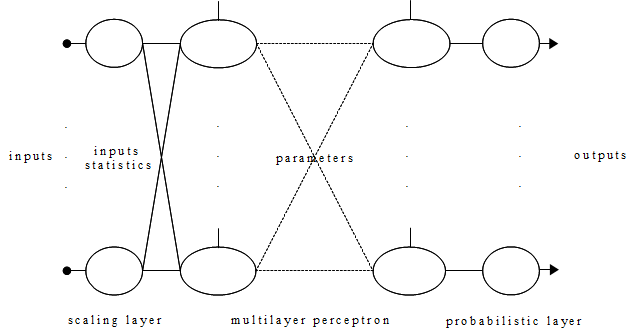
\includegraphics[width=1.2\textwidth]{pattern_recognition/neural_network_pattern_recognition.png}
\caption{Neural network for pattern recognition.}\label{NeuralNetworkPatternRecognitionFigure}
\end{center}
\end{figure}

In general, a multilayer perceptron with two layers is enough. 
A common activation function for the first layer is a sigmoid, such as the hyperbolic tangent or the logistic. 
Let us consider the activation function which should be used for the output layer. 

If the number of classes is two, the number of outputs in the neural network will be one. 
Therefore, a logistic activation function will interpret the outputs as probabilities, since it lies in the range $(0,1)$,
and no probabilistic layer is needed here. 

For multiple classes, we can use a multilayer perceptron with linear output layer. 
A probabilistic layer with softmax method is then added to form the neural network in Figure \ref{NeuralNetworkPatternRecognitionFigure}.

\subsection*{Performance functional}

In pattern recognition problems, the performance functional evaluates quantitatively the performance of the pattern recognition function against the data set. 
It is of the form

\begin{eqnarray}\label{PerformanceFunctionalPatternRecognition}\nonumber
\text{performance functional}=\text{objective term}+\text{regularization term}.
\end{eqnarray}

Common objective functionals for function regression, such as the sum squared error, the mean squared error, the root mean squared error, the normalized squared error and the Minkowski error are also commonly applied for pattern recognition. 
However, there are specific problems for this learning task, such as the cross-entropy error.

\subsection*{Training strategy}

The training algorithm for pattern recognition problems applies in the same way as for function regression problems. 

\subsection*{Model selection}

The problems of underfitting and overfitting also might occur when solving a pattern recognition problem with a neural network. 
Underfitting is explained in terms of a too simple decision boundary which gives poor separation of the training data. 
On the other hand, overfitting is explained in terms of a too complex decision boundary which achieves good separation of the training
data, but exhibits poor generalization.

A method for preventing underfitting and overfitting is to use a network that is just large enough to provide an adequate fit. 
An alternative approach to obtain good generalization is by using regularization theory.

As in function regression, early stopping can also be performed in pattern recognition to prevent overfitting. 
However, this technique usually produces underfitting and a more precise model selection analysis is preferible. 

\subsection*{Testing analysis}


The classification accuracy, error rate, sensitivity, specifity positive likelihood and negative likelihood are parameters for testing the performance of a pattern recognition problem with two classes. 

The classification accuracy is the ratio of instances correctly classified,  

\begin{eqnarray}\nonumber
\text{classification accuracy} = \frac{\text{true positives} + \text{true negatives}}{\text{true positives}+\text{true negatives}+\text{false positives}+\text{false negatives}}.
\end{eqnarray}

The error rate is the ratio of instances misclassified, 

\begin{eqnarray}\nonumber
\text{error rate} = \frac{\text{false positives} + \text{false negatives}}{\text{true positives}+\text{true negatives}+\text{false positives}+\text{false negatives}}.
\end{eqnarray}

The sensitivity, or true positive rate, is the proportion of alcual positive which are predicted positive, 

\begin{eqnarray}\nonumber
\text{sensitivity} = \frac{\text{true positives}}{\text{true positives}+\text{false positives}}.
\end{eqnarray}


The specifity, or true negative rate, is the proportion of actual negative which are predicted negative, 

\begin{eqnarray}\nonumber
\text{specifity} = \frac{\text{true negatives}}{\text{true negatives}+\text{false positives}}.
\end{eqnarray}
 
The positive likelihood is the likelihood that a predicted positive is an actual positive

\begin{eqnarray}\nonumber\label{PositiveLikelihood}
\text{positive likelihood} = \frac{sensitivity}{1-specifity}.
\end{eqnarray}

The negative likelihood is the likelihood that a predicted negative is an actual negative

\begin{eqnarray}\nonumber
\text{negative likelihood}= \frac{specifity}{1-sensitivity}.
\end{eqnarray}

Table \ref{BinaryClassificationPerformanceVariables} summarizes the binary classification performance variables

\begin{table}[h!]
\begin{center}
\begin{tabular}{c}
\hline
Classification accuracy\\
Error rate\\
Sensitivity\\
Specifity\\
True positive rate\\
True negative rate\\
\hline
\end{tabular}\caption{Binary classification performance variables.}
\label{BinaryClassificationPerformanceVariables}
\end{center}
\end{table}


In the confusion matrix the rows represent the target classes and the columns the output classes for a testing target data set. The diagonal cells in each table show the number of cases that were correctly
classified, and the off-diagonal cells show the misclassified cases. 

For the case of two classes the confusion matrix takes the form

\begin{eqnarray}\nonumber
\mathbf{C} = 
\left(
\begin{array}{cc}
\text{true positives} & \text{false positives} \\
\text{false negatives} & \text{true negatives} \\
\end{array}
\right).
\end{eqnarray}

% ROC CURVES



\section{Examples}\label{ExamplesPatternRecognition}
\subsection*{Simple pattern recognition}

This is an academic example defined by a data set with $100$ instances, $2$ inputs, or attributes, and $1$ target. 
The target variable represents two classes ($0$ and $1$). 
The aim is to design a neural network that can predict the correct class for given attribute values. 
Figure \ref{SimplePatternRecognitionFigure} shows this data set.

\begin{figure}[!hbp]
\begin{center}
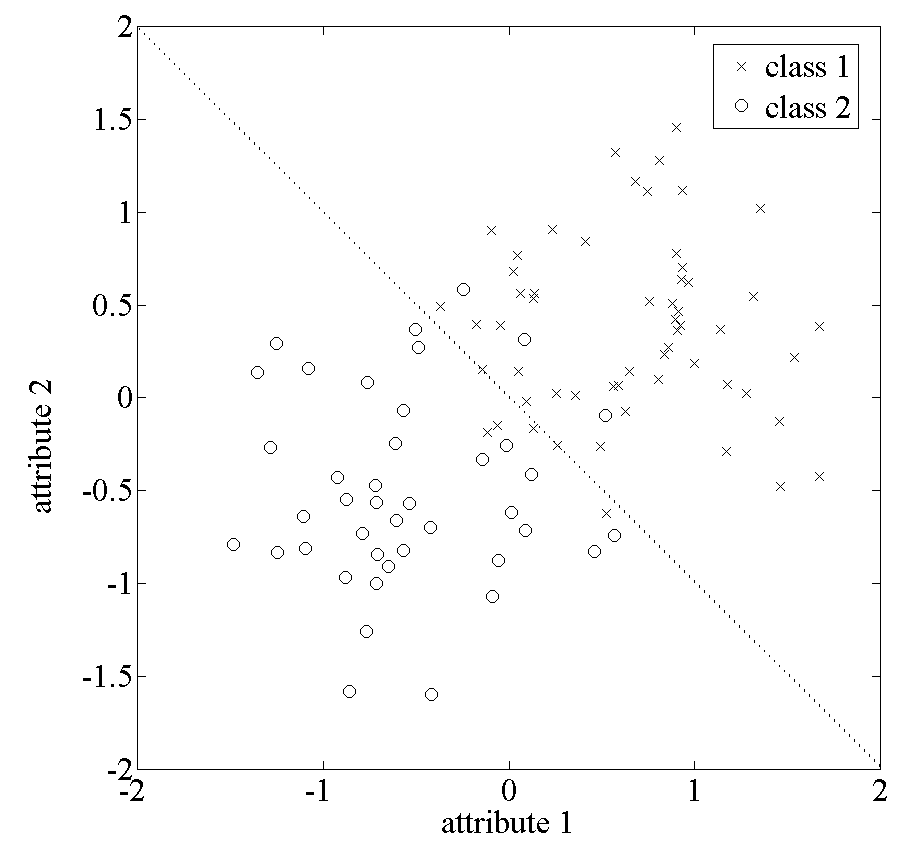
\includegraphics[width=0.75\textwidth]{pattern_recognition/simple_pattern_recognition_data_set.png}
\caption{Data set for the simple pattern recognition example.}\label{SimplePatternRecognitionFigure}
\end{center}
\end{figure}

\subsection*{Iris plant}

This is perhaps the best known data set to be found in the pattern recognition literature. 
It contains $3$ classes of $50$ instances each, where each class refers to a type of iris plant. 
One class is linearly separable from the other two; the latter are not linearly separable from each other.
Figure \ref{IrisPlantFigure} illustrates this example. That picture is has been taken from Wikipedia.  

\begin{figure}[!hbp]
\begin{center}
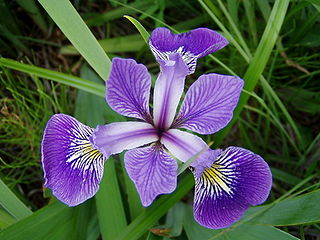
\includegraphics[width=0.6\textwidth]{pattern_recognition/iris_versicolor}
\caption{Iris versicolor.}\label{IrisPlantFigure}
\end{center}
\end{figure}

The input variables are:

\begin{enumerate}
\item Sepal length, in centimeters.
\item Sepal width, in centimeters.
\item Petal length, in centimeters.
\item Petal width, in centimeters.
\item Class -iris setosa, iris versicolour or iris virginica.
\end{enumerate}

The predicted class is the class of iris plant:
 
\begin{enumerate}
\item Iris setosa (true or false).
\item Iris versicolour (true or false).
\item Iris virginica (true or false).
\end{enumerate}

More information on this problem can be found in \cite{UCI}.

\subsection*{Pima indians diabetes}

Pima Indians of Arizona have the population with the highest rate of diabetics in the world. 
It has been estimated that around $50\%$ of adults suffer from this disease. 
The aim of this pattern recognition problem is to predict whether an individual of Pima Indian heritage has diabetes from personal characteristics and physical measurements.
Figure \ref{BloodGlucoseTestingFigure} is a blood glucose testing device, showed here to illustrate this example. 
That picture has been taken from Wikipedia. 

\begin{figure}[!hbp]
\begin{center}
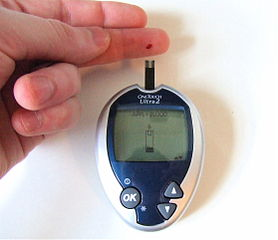
\includegraphics[width=0.5\textwidth]{pattern_recognition/blood_glucose_testing}
\caption{Blood glucose testing.}\label{BloodGlucoseTestingFigure}
\end{center}
\end{figure}


The data is taken from the UCI Machine Learning Repository
\cite{UCI}. The number of samples in the data set is $768$.
The number of input variables for each sample is $8$. All input
variables are numeric-valued, and represent personal
characteristics and physical measurements of an individual. The
number of target variables is $1$, and represents the absence or
presence of diabetes in an individual. Table
\ref{DataSetInformation} summarizes the 
data set information, while tables \ref{InputVariablesInformation}
and \ref{TargetVariablesInformation} depict the input and target
variables information, respectively.

\begin{table}[h!]
\begin{center}
\begin{tabular}{cc}
\hline
Number of instances: & $768$ \\
Number of input variables: & $8$ \\
Number of target variables: & $1$ \\
\hline
\end{tabular}\caption{Data set information.}\label{DataSetInformation}
\end{center}
\end{table}


\begin{table}[h!]
\begin{center}
\begin{tabular}{cc}
\hline
1. & Number of times pregnant.\\
2. & Plasma glucose concentration a 2 hours in an oral glucose tolerance test.\\
3. & Diastolic blood pressure ($mm Hg$).  \\
4. & Triceps skin fold thickness ($mm$).  \\
5. & 2-Hour serum insulin ($mu U/ml$). \\
6. & Body mass index (weight in $kg$/(height in $m$)$^2$). \\
7. & Diabetes pedigree function. \\
8. & Age (years). \\
\hline
\end{tabular}\caption{Input variables information.}\label{InputVariablesInformation}
\end{center}
\end{table}

\begin{table}[h!]
\begin{center}
\begin{tabular}{cc}
\hline
1. & Absence or presence of diabetes (0 or 1). \\
\hline
\end{tabular}\caption{Target variables information.}\label{TargetVariablesInformation}
\end{center}
\end{table}



%%%%%%%%%%%%%%%%%%%%%%%%%%%%%%%%%%%%%%%%%%%%%%%%%%%%%%%%%%%%%%%%%%%%%%%%%%%%%%%%%%%%

\chapter{Optimal control}\label{OptimalControl}
Optimal control is also a learning tasks for neural networks. 
\texttt{OpenNN} classes which are related to the solution of optimal control problems include the mathematical model and  
several performance term classes. 



\section{Basic theory}\label{BasicTheoryOptimalControl}
Optimal control -which is playing an increasingly important role in
the design of modern systems- has as its aim the optimization,
in some defined sense, of physical processes. 
More specifically, the
objective of optimal control is to determine the control signals
that will cause a process to satisfy the physical constraints and at
the same time minimize or maximize some performance criterion
\cite{Kirk1970}.

The formulation of an optimal control problem requires:

\begin{itemize}
\item[-] A mathematical model.
\item[-] A neural network.
\item[-] A performance functional.
\item[-] A training strategys.
\end{itemize}

\subsection*{Mathematical model}\index{mathematical model}
\index{state variable}
\index{control variable}
\index{state equation}
\index{algebraic operator}
\index{differential operator}
\index{forcing term}

The model of a process is a mathematical description that
adequately predicts the response of the physical system to all
anticipated inputs.

A mathematical model (or state equation) contains state variables and control variables. 
Mathematical models can be expressed as all algebraic, ordinary differential and partial differential equations. 
However, many optimal control problems in the literature are based on mathematical models described by a system of ordinary differential equations together with their respective initial conditions, representing a dynamical model of the system. 
Integration here is usually performed with the Runge-Kutta-Fehlberg method.

\subsection*{Neural network}
\index{input constraint}
\index{control constraint}
\index{state constraint}
\index{boundary condition}
\index{lower and upper bounds}
\index{admissible control}

A neural network is used to represent the control variables. 
The number of inputs is usually one, which represents the time, and the number of outputs is normally small, representing the control variables. 
Although the number of hidden layers and the sizes of each are design variables, that is not a critical issue in optimal control. 
Indeed, this class of problems are regarded as being well-possed, 
and a sufficient complexity for the function space selected is generally enough. 

Figure \ref{NeuralNetworkOptimalControlFigure} shows a neural network template for solving optimal control problems. 

\begin{figure}[h!]
\begin{center}
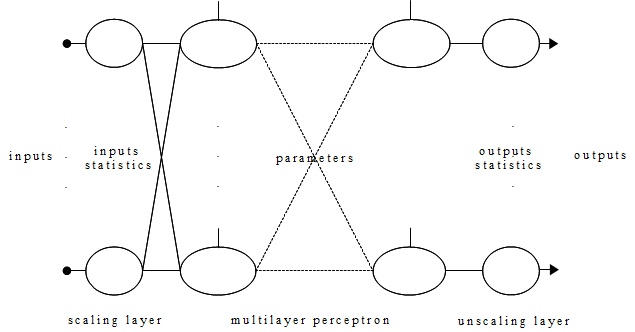
\includegraphics[width=1.2\textwidth]{optimal_control/neural_network_optimal_control.png}
\caption{Neural network for optimal control.}\label{NeuralNetworkOptimalControlFigure}
\end{center}
\end{figure}

An optimal control problem might be specified by a set of constraints on the control variables. 
Two important types of control constraints are boundary conditions and lower and upper bounds. 

If some outputs are specified for given
inputs, then the problem is said to include boundary
conditions. On the other hand, if some
control variables are restricted to fall in some interval, then the
problem is said to have lower and upper bounds.

Also, some optimal control problems need a neural network with associated independent parameters. 
The most common are those with free final time.

\subsection*{Performance functional}
\index{performance criterion, see objective functional}
\index{admissible state}

The performance functional of an optimal control problem always includes an objective term.
It might also include a regularization and a constraints terms,  

\begin{eqnarray}\nonumber
\text{Performance functional = objective term + regularization term + constraints term}. 
\end{eqnarray}

In certain cases the problem statement might clearly indicate which
objective criterion is to be selected, whereas in other cases that
selection is a subjective matter \cite{Kirk1970}.

The regularization term makes the control variables to have smoother shapes. 

State constraints are conditions that the physical system must
satisfy. This type of constraints vary according to the problem at
hand.

In this way, a control which satisfies all the control and state
constraints is called an admissible control \cite{Kirk1970}.

Similarly, a state which satisfies the state constraints is called
an admissible state \cite{Kirk1970}.

An optimal control is defined as one that minimizes or maximizes the
performance criterion, and the corresponding state is called an
optimal state. In this way, the problem of optimal control is formulated as a
variational problem \cite{Kirk1970}.

In general, the performance function, cannot be evaluated analytically. 
This makes that the gradient vector and the Hessian matrix can neither be computed analytically, and numerical differentiation must be used. 

\subsection*{Training strategy}

We have seen that the performance functional for optimal control problems might contain up to three terms: 
objective, regularization and constraints. On the other hand, in most of the cases, it cannot be computed analitycally. 
That makes that a single training algorithm might not fully converge if the solution is far away from the optimal one. 

Therefore, when solving optimal control problems, it is recommended to use an initialization training algorithm before the main training process. 
The form of the training strategy is therefore as follows:

\begin{eqnarray}\nonumber
\text{Training strategy: initialization training algorithm, main training algorithm}. 
\end{eqnarray}

The initialization training algorithm is usually a zero order algorithm, such as random search or the evolutionary algorithm;
the main training algorithm might be a first order algorithm, such as conjugate gradient or the quasi-Newton method. 


\section{Examples}\label{ExamplesOptimalControl}
\subsection*{Car problem}

Consider a car which is to be driven along the x-axis from some initial position and
velocity to some desired position and velocity in a minimum time see Figure \ref{CarProblemFigure}.
 
\begin{figure}[h!]
\begin{center}
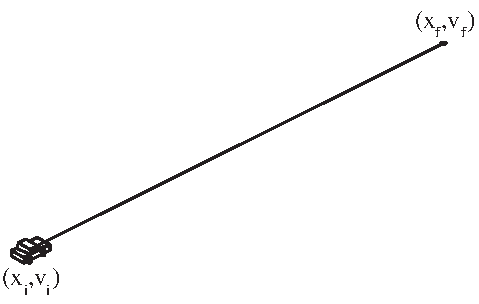
\includegraphics[width=0.6\textwidth]{optimal_control/car_problem_statement}
\caption{Car problem statement.}\label{CarProblemFigure}
\end{center}
\end{figure}
 
 
To simplify the problem, let us approximate the car by a unit point mass
that can be accelerated by using the throttle or decelerated by using the
brake. 
Selecting position and velocity as state variables the mathematical
model of this system becomes a problem of two ordinary differential
equations with their corresponding initial conditions.

The acceleration is bounded by the capability of the engine, and the
deceleration is limited by the braking system parameters. 

As the objective is to make the car reach the final point as quickly as
possible, the objective functional for this problem is given by the final time.

On the other hand, the car is to be driven to a desired position and a
desired velocity. The erros in that target position and velocity are the constraints of the problem.

The statement and the solution itself of this car problem points out a
number of significant issues. First, some variational problems might require
a function space with independent parameters associated to it. Indeed, the
final time is not part of the control, but it represents the interval when it is
defined. Finally, this kind of applications demand spaces of functions with
very good approximation properties, since they are likely to have very non-
linear solutions. Here the optimal control even exhibits discontinuities.


\subsection*{Car problem neurocomputing}

This problem is very similar to the one above. 
It can be formulated as an optimal control problem with one control and two state variables, 
and where the control is subject to two boundary conditions and lower and upper bounds. 
The performance functional has one constraint and requires the integration of a system of two ordinary differential equations. 

Therefore, there main differences between these two car problems are in the number of control variables and in the characteristics of them.
In the problem above the number of control variables is two (acceleration and deceleration), while that in this problem there is just one (acceleration, which can be negative to represent deceleration).
On the other hand, in the problems above, the variables are not subject to any condition,while here the acceleration must be zero at both the initial and final times.

\subsection*{Fed batch fermenter}

The fed batch fermenter problem formulated in this section is an optimal
control problem with one control and four state variables, and defined by
a performance functional with one constraint and requiring the integration
of a system of ordinary differential equations. 

In many biochemical processes, the reactors are operated in fed batch mode,
where the feed rate into the reactor is used for control. 
There is no outflow, so the feed rate must be chosen so that that batch volume does not exceed
the physical volume of the reactor.
As a specific example, an optimization study of the fed batch fermentation
for ethanol production by Saccharomyces cerevisiae is presented.
Figure \ref{EthanolPlantFigure}, taken from Wikipedia, is a picture of a ethanol plant. 

\begin{figure}[!hbp]
\begin{center}
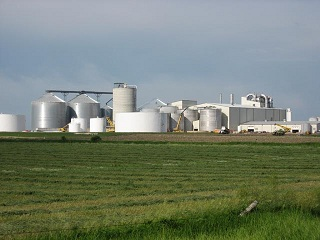
\includegraphics[width=0.7\textwidth]{optimal_control/ethanol_plant}
\caption{Chemical plant for ethanol production.}\label{EthanolPlantFigure}
\end{center}
\end{figure}


The fed batch fermentation process considered here is a process in which
ethanol is produced by Saccharomyces cerevisiae and the production of ethanol
is inhibited by itself.

A batch fermenter generally consists of a closed vessel provided with a
means of stirring and with temperature control. It may be held at constant
pressure or it can be entirely enclosed at a constant volume. In many biochemical processes, 
the reactors are operated in fed batch mode, where the
feed rate into the reactor chosen so that that batch volume does not exceed
the physical volume of the reactor \cite{Luus1993}. 

The states of the plant are the concentration of cell mass, the concentration of substrate, 
the concentration of product and the broth volume in the fermenter. 
The control variable is the feeding rate, and it is
is the only manipulated variable of this process \cite{Luus1993}. 

The dynamic behavior of this fed batch fermentation process can be described by four differential-algebraic equations,
together with their initial conditions. 

The liquid volume of the reactor is limited by the vessel size. This
constraint on the state of the system can be written as an error functional.

The desired objective is to obtain a maximum amount of yield at the end of
the process. The actual yield in the reactor is given by the concentration of
product multiplied by the broth volume in the reactor. 

Since the equations describing the fermenter are nonlinear and the inputs
and states are constrained, the determination of the feed rate to maximize
the yield can be quite difficult.


\subsection*{Aircraft landing}

This is an optimal control problem of aeronautical engineering interest, with one control and
four state variables, and where the objective functional is evaluated by integrating a system of
four ordinary differential equations.

The landing of an aircraft consists of two main stages: the
glide-path phase and the flare-out phase. Here we seek to determine the optimal control and the
corresponding optimal trajectory of an aircraft during its final
approach before landing. 
Figure \ref{AircraftLandingFigure} illustrates the landing process of an aircraft. 
That picture is taken from Wikipedia. 

\begin{figure}[!hbp]
\begin{center}
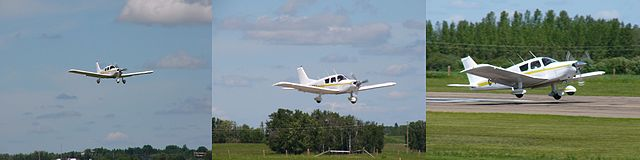
\includegraphics[width=1.0\textwidth]{optimal_control/aircraft_landing}
\caption{Landing of an aircraft.}\label{AircraftLandingFigure}
\end{center}
\end{figure}

The aircraft landing problem examined here is similar to that considered in \cite{Ellert1963}.

In the flare-out phase the longitudinal dynamics of the aircraft
are governed by the pitch angle, which in turn is controlled by the elevator deflection angle \cite{Ashley1992}. 


Figure \ref{AircraftAngles} depicts the
pitch and the elevator deflection angles of an aircraft.

\begin{figure}[h!]
\begin{center}
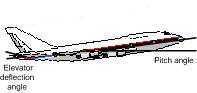
\includegraphics[width=0.5\textwidth]{optimal_control/aircraft_angles.jpg}
\caption{Elevator deflection angle and pitch angle.}\label{AircraftAngles}
\end{center}
\end{figure}

Thus the aim of the aircraft landing problem considered here is to
determine an optimal elevator deflection angle as a function of
time that satisfies a set of performance requirements.

As stated earlier, the elevator controls the longitudinal motion
of the aircraft. It is assumed that any control signal is
instantaneously represented by the elevator. The elevator
deflection angle is also physically limited to a finite range.

The following variables will be used to describe the dynamics of the aircraft \cite{Ellert1963}:
the pitch angle rate, the pitch angle, the altitude rate and, the altitude. 

The velocity of the aircraft and it is assumed to be constant during the flare-out phase. 

The mathematical model shows that the elevator deflection angle
has a direct effect on the pitch angle rate,
which in turn affects the pitch angle, the altitude
rate and the altitude.

The performance requirements define the physical constraints and
desired values of the control and the state variables. The most
important requirements and constraints for the landing system
considered in this problem are highlighted in the following section.

In our example problem the flare-out procedure ends at the final or touchdown time. 

During a process it is often desirable to be able to define the
desired value of a given state variable; this information can then
be used to evaluate the performance of the system. The desired
altitude of the aircraft is the most visual characteristic of the
landing procedure. For this problem it is given by Figure
\ref{DesiredAltitudeFigure}.

\begin{figure}[h!]
\begin{center}
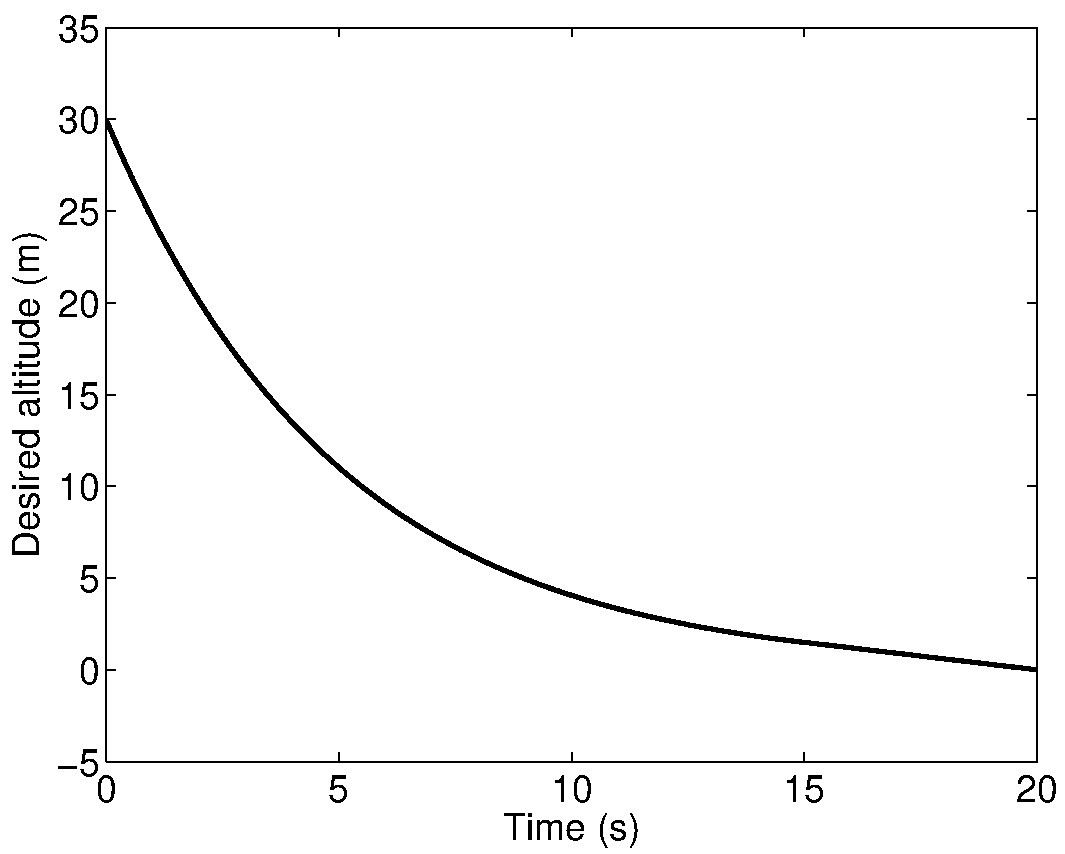
\includegraphics[width=0.6\textwidth]{optimal_control/target_altitude_aircraft_landing}
\caption{Desired landing altitude.}\label{DesiredAltitudeFigure}
\end{center}
\end{figure}

It is desirable to land without expending excessive amounts of
control effort. Therefore, a regularization term can be added. 

At the time of touchdown the pitch angle of the aircraft must lie
in an appropriate range. This requirement is
defined by a set of physical limitations. The lower limit serves
to ensure the nose wheel of a tricycle landing gear does not
touchdown prematurely. Similarly the upper limit is set to prevent
the tail gear touching downing first. A desired pitch angle at
touchdown could be specified as a constraints term. 





 
%%%%%%%%%%%%%%%%%%%%%%%%%%%%%%%%%%%%%%%%%%%%%%%%%%%%%%%%%%%%%%%%%%%%%%%%%%%%%%%%%%%%
 
\chapter{Optimal shape design}\label{OptimalShapeDesign}
Optimal shape design is another learning tasks for neural networks. 
That problem type is formulated in a very similar way than optimal control. 
\texttt{OpenNN} classes which are related to the solution of optimal shape design problems include the mathematical model and  
several performance term classes. 



\section{Basic theory}\label{BasicTheoryOptimalShapeDesign}
Optimal shape design is a very interesting field both mathematically
and for industrial applications. The goal here is to computerize the
design process and therefore shorten the time it takes to design or
improve some existing design. In an optimal shape design process one
wishes to optimize a criteria involving the solution of some
mathematical model with respect to its domain of definition
\cite{Mohammadi2004}. The detailed study of this subject is at the
interface of variational calculus and numerical analysis.

%For instance the design of a harbor which minimizes the waves
%coming from far can be done at little cost by standard
%optimization methods once the numerical simulation of Helmholtz
%equation is mastered.
%
%Weight reduction in car engine, aircraft structures, etc
%Electromagnetically optimal shapes, such as in stealth airplanes
%Wave canceling fore bulbe in boat design Drag reduction for
%airplanes,cars and boats. An example of an optimal shape design
%problem could be the design of flow aerofoil sections.

%Optimal Shape Design is concerned with the optimization of some
%performance criterion dependent (besides the constraints of the
%problem) on the physical form of some region (device).

%Optimal Shape Design has developed over the years, from the
%abstract field of calculus of variations to applications in
%structure mechanics and fluid mechanics becoming now a valuable
%tool for the design optimization of airplanes. Weight reduction,
%stress reinforcement, drag reduction and even noise reduction can
%be obtained. The field is said to have started with Hadamard[8]
%who gave the first formula to evaluate the change due to a
%boundary modification of the domain of a partial differential
%equation.

In order to properly define an optimal shape design problem the
following concepts are needed:

\begin{enumerate}
\item Mathematical model.
\item Neural network.
\item Performance functional. 
\item Training strategy.
\end{enumerate}

\subsection*{Mathematical model}
\index{mathematical model}
\index{shape variable}
\index{state variable}
\index{state equation}

The mathematical model or state equation is a well-formed formula which involves the
physical form of the device to be optimized. 
It contains shape variables and state variables. 

A mathematical model might be described by algebraic equations, ordinary differential equations or partial differential equations. 

\subsection*{Neural network}
\index{shape constraint}
\index{boundary condition}
\index{lower and upper bounds} 

A neural network is used to represent the shape variables. 
Optimal shape design problems are usually defined by constraints on the shape function. 
Two important types of shape constraints are boundary conditions and lower and upper bounds. 

\subsection*{Performance functional}
\index{state constraint}
\index{admissible shape}
\index{admissible state}

The performance functional of an optimal shape design problem always includes an objective term.
It usually includes a constraints term,  

\begin{eqnarray}\nonumber
\text{Performance functional = objective term + constraints term}. 
\end{eqnarray}


An optimal shape design problem might also be specified by a set of
constraints on the state variables of the
device.

State constraints are conditions that the solution to the problem
must satisfy. This type of constraints vary according to the problem
at hand.

In this way, a design which satisfies all the shape and state
constraints is called an admissible shape.

Similarly, a state which satisfies the constraints is called an
admissible state.

The performance criterion expresses how well a given design does the
activity for which it has been built.


Optimal shape design problems solved in practice are, as a rule,
multi-criterion problems. This property is
typical when optimizing the device as a whole, considering, for
example, weight, operational reliability, costs, etc. It would be
desirable to create a device that has extreme values for each of
these properties. However, by virtue of contradictory of separate
criteria, it is impossible to create devices for which each of them
equals its extreme value.


\subsection*{Trainining strategy}

The performance functional for optimal shape design problems might contain up to three terms: 
objective, regularization and constraints. 
On the other hand, in most of the cases, it cannot be computed analitycally. 
That makes that a single training algorithm might not fully converge if the solution is far away from the optimal one. 

Therefore, when solving optimal shape design problems, it is recommended to use an initialization training algorithm before the main training process. 
The form of the training strategy is therefore as follows:

\begin{eqnarray}\nonumber
\text{Training strategy: initialization training algorithm, main training algorithm}. 
\end{eqnarray}

The initialization training algorithm is usually a zero order algorithm, such as random search or the evolutionary algorithm;
the main training algorithm might be a first order algorithm, such as conjugate gradient or the quasi-Newton method. 


\section{Examples}\label{ExamplesOptimalShapeDesign}
\subsubsection*{Minimum drag problem}

The minimum drag problem formulated here an optimal shape
design problem with one input and one output variables, besides two boundary conditions. 
It is defined by an unconstrained objective functional requiring the integration of a function. 

Consider the design of a body of revolution with given length and diameter providing minimum drag at zero angle of attack and for neglected friction
effects. 
Figure \ref{SpaceShuttleFigure} is a picture of a space shuttle, which could be that body of revolution. 
That picture is taken from Wikipedia. 

\begin{figure}[h!]
\begin{center}
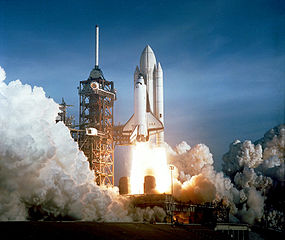
\includegraphics[width=0.7\textwidth]{optimal_shape_design/space_shuttle}
\caption{Space shuttle.}\label{SpaceShuttleFigure}
\end{center}
\end{figure}

For a slender body, the pressure coefficient can be approximated by the Newtonian flow relation.
The Newtonian flor provides us with a simple approximation for the drag.



%%%%%%%%%%%%%%%%%%%%%%%%%%%%%%%%%%%%%%%%%%%%%%%%%%%%%%%%%%%%%%%%%%%%%%%%%%%%%%%%%%%%
 
\chapter{Inverse problems}\label{InverseProblems}
Iverse problems are the most complex applications for neural networks, 
since learning is performed here from both mathematical models and data sets. 
\texttt{OpenNN} classes which are related to the solution of inverse problems include the mathematical model, the data set,  
several performance term classes and the testing analysis classes. 



\section{Basic theory}\label{BasicTheoryInverseProblems}
Inverse problems can be described as being opposed to direct
problems. In a direct problem the cause is given, and the effect is
determined. In an inverse problem the effect is given, and the cause
is estimated \cite{Kirsch1996}. There are two main types of inverse
problems: input estimation, in which the system properties and
output are known and the input is to be estimated; and properties
estimation, in which the the system input and output are known and
the properties are to be estimated \cite{Kirsch1996}. Inverse
problems are found in many areas of science and engineering.

%Inverse problems are those where a set of measured results is
%analyzed in order to get as much information as possible on a model
%which is proposed to represent a system in the real world. Exact
%inverse problems are related to most parts of mathematics. Applied
%inverse problems are the keys to other sciences. Hence the field,
%which is very wealthy, yields the best example of interdisciplinary
%research but it has nevertheless a strong individuality. The
%obtained results and explored directions of the 20th century are
%sketched in this review, with attempts to predict their evolution.
%
%Inverse problems are the problems that consist of finding an
%unknown property of an object, or a medium, from the observation
%of a response of this object, or medium, to a probing signal.
%Thus, the theory of inverse problems yields a theoretical basis
%for remote sensing and non-destructive evaluation
%\cite{Ramm2005}.

%For example, if an acoustic plane wave is scattered by an
%obstacle, and one observes the scattered field far from the
%obstacle, or in some exterior region, then the inverse problem is
%to find the shape and material properties of the obstacle. Such
%problems are important in identification of flying objects
%(airplanes missiles, etc.), objects immersed in water (submarines,
%paces of fish, etc.), and in many other situations. In geophysics
%one sends an acoustic wave from the surface of the earth and
%collects the scattered field on the surface for various positions
%of the source of the field for a fixed frequency, or for several
%frequencies. The inverse problem is to find the subsurface
%inhomogeneities. In technology one measures the eigenfrequencies
%of a piece of a material, and the inverse problem is to find a
%defect in this material, for example, a hole in a metal. In
%geophysics the inhomogeneity can be an oil deposit, a cave, a
%mine. In medicine it may be a tumor, or some abnormality in a
%human body. If one is able to find inhomogeneities in a medium by
%processing the scattered field on the surface, then one does not
%have to drill a hole in a medium. This, in turn, avoids expensive
%and destructive evaluation. The practical advantages of remote
%sensing are what makes the inverse problems important
%\cite{Ramm2005}.

An inverse problem is specified by the following concepts:

\begin{itemize}
\item[-] Mathematical model.
\item[-] Data set.
\item[-] Neural network.
\item[-] Performance functional.
\item[-] Training strategy.
\end{itemize}

\subsubsection*{Mathematical model}
\index{mathematical model}
\index{unknown variable}
\index{state variable}
\index{algebraic operator}
\index{differential operator}
\index{forcing term}

The mathematical model can be defined as a representation of the
essential aspects of some system which presents knowledge of that
system in usable form.

%Let us represent $\mathbf{y}(\mathbf{x})$ the vector of unknowns
%(inputs or properties) and
%$\mathbf{u}(\mathbf{x})$ the vector of state variables. The mathematical model, or state equation, relating
%unknown and state variables takes the form

%\begin{eqnarray}\label{InputEstimationEquation}
%\mathcal{L}(\mathbf{y}(\mathbf{x}),
%\mathbf{u}(\mathbf{x}),\mathbf{x}) = \mathbf{f},
%\end{eqnarray}

%\noindent where $\mathcal{L}$ is some algebraic or differential
%operator and $\mathbf{f}$ is some forcing term.


%The variables of an inverse problem, i.e., variables which describe
%the characteristics of the device for which the problem is
%specified, are interrelated according to the following operator
%equation \cite{Korovkin2007}:

%Equation (\ref{InverseProblemsEquation}) provides a means to
%calculate the variables $\mathbf{w}$ of the inverse problem for
%any $\mathbf{p}$.

\subsubsection*{Data set}
\index{observed data}

Inverse problems are those where a set of measured results is
analyzed in order to get as much information as possible on a
mathematical model which is proposed to represent a real system.

Therefore, a data set on the state variables is
needed in order to estimate the unknown variables of that system.

In general, that data set is invariably affected by noise and
uncertainty, which will translate into uncertainties in the system
inputs or properties.

\subsubsection*{Neural network}
\index{unknowns constraint}

The neural network represents here the inputs to the system or the properties of that system. 
They might include boundary conditions or bounds. 

\subsubsection*{Performance functional}
\index{state constraint}
\index{input constraint}\index{property constraint}
\index{boundary condition}\index{lower and upper bounds}
\index{admissible unknown}
\index{admissible state}

For inverse problems, the presence of restrictions is typical. 
State constraints are those conditions that the system needs to
hold. This type of restrictions depend on the particular problem.

In this way, an unknown which satisfies all the input and state
constraints is called an admissible unknown.


Also, a state which satisfies the state constraints is called an
admissible state.

The inverse problem provides a link between the outputs from the
model and the observed data. When formulating and solving inverse
problems the concept of error functional is used to specify the
proximity of the state variable to the
observed data.


Some common performance functionals for invers problems are the inverse sum squared
error or the inverse Minkowski error. Regularization
theory can also be applied here
\cite{Bucur2005}.

The solution of inverse problems is then reduced to finding the
extremum of a functional.

On the other hand, inverse problems might be ill-posed
\cite{Tikhonov1977}. A problem is said to be
well possed if the following conditions are true: (a) the solution to the problem exists;
(b) the solution is unique; and (c) the solution
is stable. This implies that for the
above-considered problems, these conditions can be violated.
Therefore, their solution requires application of special methods.
In this regard, the use of regularization theory is widely used
\cite{Engl2000}.

In some elementary cases, it is possible to establish analytic
connections between the sought inputs or properties and the observed
data. But for the majority of cases the search of extrema for the
error functional must be carried out numerically, and the so-called
direct methods can be applied.

\subsubsection*{Training strategy}

The training strategy is entrusted to solve the reduced function optimization problems. 
When possible, a quasi-Newton problem should be used. 
If the gradient of the performance function cannot be computed accurately, an evolutionary algorithm could be used instead. 



\section{Examples}\label{ExamplesInverseProblems}
\subsubsection*{Precipitate dissolution modeling}

This is an property estimation problem with one input variable, one output variable and one independent parameter. 
The mathematical model here is expressed as an algebraic equation. 

The objective is to model the dissolution rate of hardening precipitates in aluminium alloys. 
The effective activation energy is also in unison determined as that providing the best results. 
Aluminium alloys 2014-T6 and 7449-T79 are considered. 
Figure \ref{VickersTesterFigure} shows a Vickers hardness tester (picture from Wikipedia). 

\begin{figure}[h!]
\begin{center}
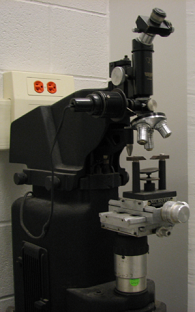
\includegraphics[width=0.5\textwidth]{inverse_problems/vickers_tester}
\caption{Vickers hardness tester.}\label{VickersTesterFigure}
\end{center}
\end{figure}

Assuming that the nucleation of precipitates is
negligible compared to the dissolution of precipitates, the
following linear relationship between the Vickers hardness and the
volumetric fraction of precipitates can be established
\cite{Myrh1991b}.

The Vickers hardness equation is extremely useful since the
hardness is much easier to measure than the relative volume
fraction of precipitates.

The dissolution modeling process is to estimate an activation
energy providing minimum dispersion for the experimental data
while a function providing minimum error.
Mathematically, this can be formulated as a variational problem
including independent parameters.

Experimental tests have been performed in order to get the
isothermal time evolution of Vickers hardness at different
temperatures and for various aluminium alloys. In particular, two
materials have been used for the isothermal heat treatments, 2014-T6
and 7449-T79 aluminium alloys.

The Vickers hardness data for aluminium alloy 2014-T6 is taken from
\cite{Shercliff2005}, while that for aluminium alloy 7449-T79 is
obtained from an independent test performed within the DEEPWELD
Specific Targeted Research Project (STREP) co-funded by the 6th
Framework Programme of the European Community (AST4-CT-2005-516134).

Figures \ref{VickersHardnessTest2014-T6} and
\ref{VickersHardnessTest7449-T79} depict these Vickers hardness test
for aluminium alloys 2014-T6 and AA7449-T6, respectively. Note that,
in both figures the Vickers hardness decreases with the time, due to
dissolution of hardness precipitates.

\begin{figure}[h!]
\begin{center}
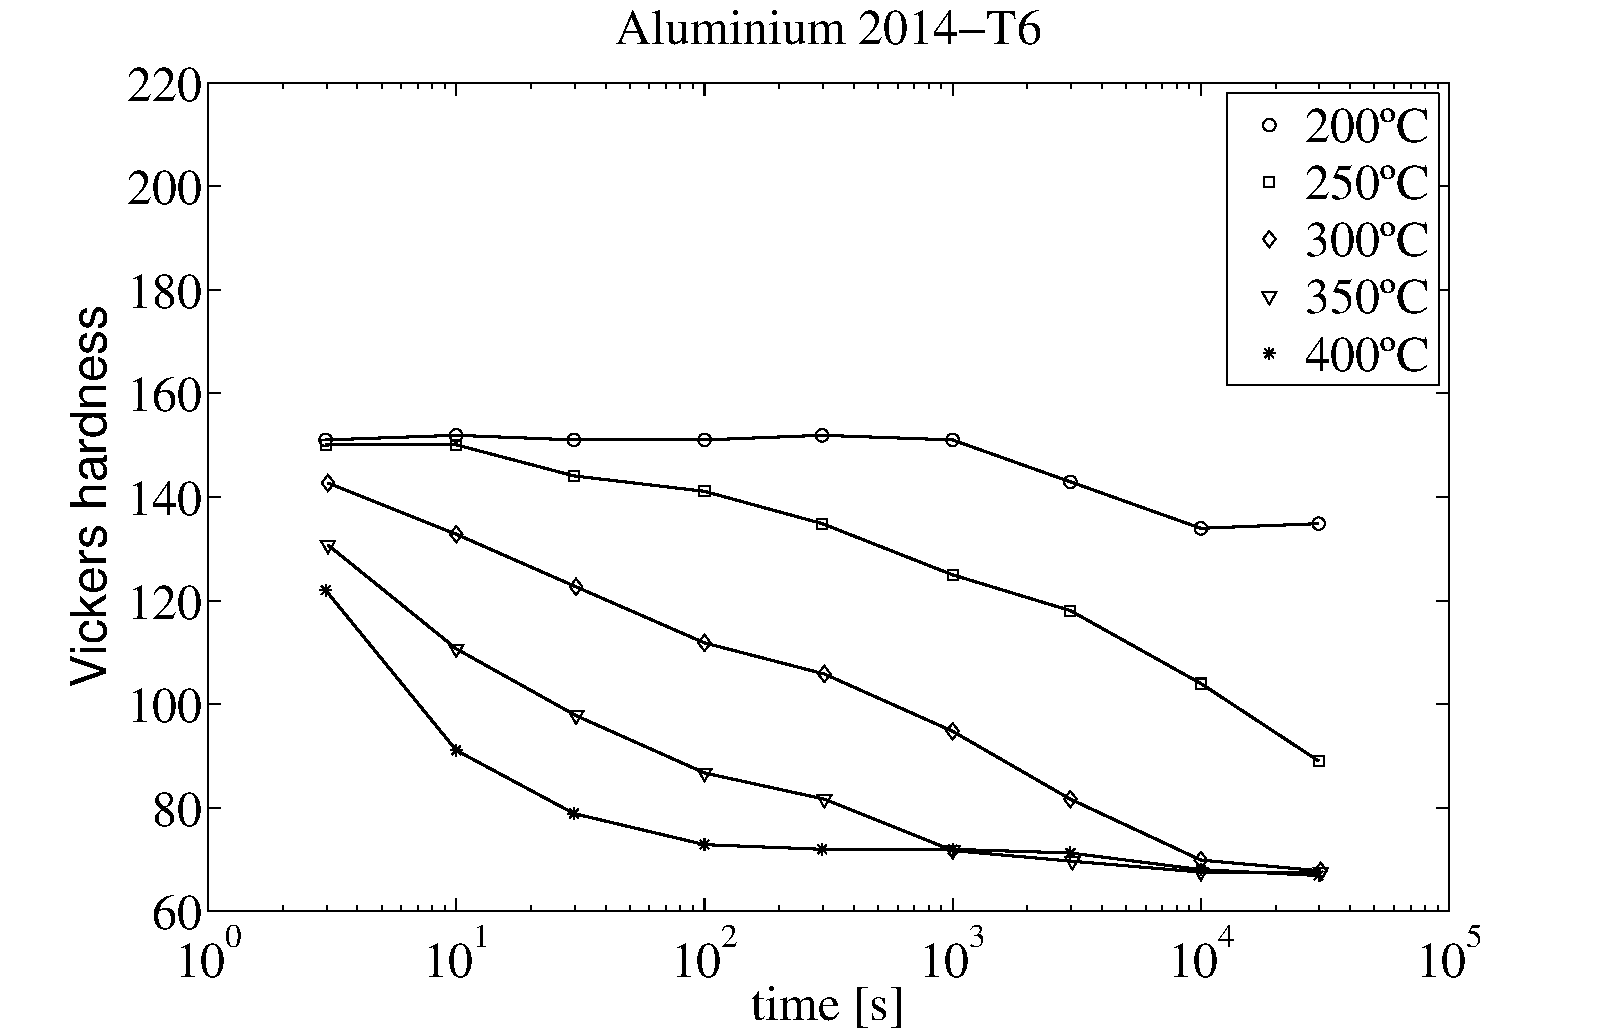
\includegraphics[width=0.9\textwidth]{inverse_problems/vickers_hardness_test_2014-T6}
\caption{Vickers hardness test for aluminium alloy
2014-T6.}\label{VickersHardnessTest2014-T6}
\end{center}
\end{figure}

\begin{figure}[h!]
\begin{center}
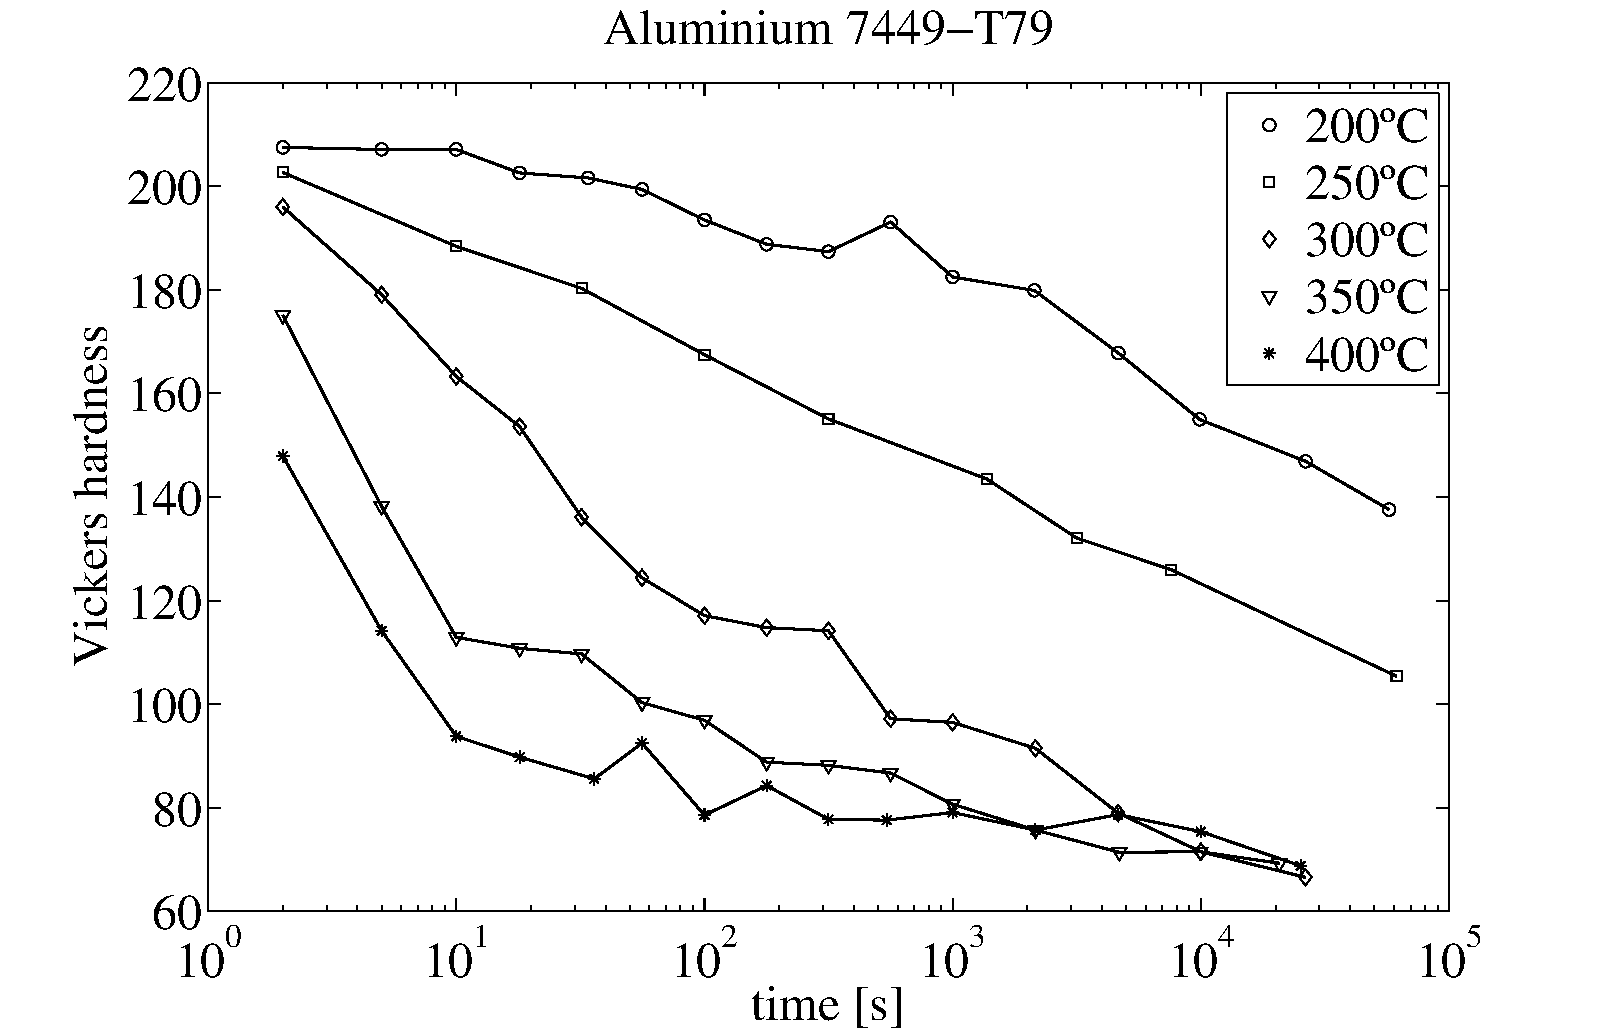
\includegraphics[width=0.9\textwidth]{inverse_problems/vickers_hardness_test_7449-T79}
\caption{Vickers hardness test for aluminium alloy
7449-T79.}\label{VickersHardnessTest7449-T79}
\end{center}
\end{figure}


%%%%%%%%%%%%%%%%%%%%%%%%%%%%%%%%%%%%%%%%%%%%%%%%%%%%%%%%%%%%%%%%%%%%%%%%%%%%%%%%%%%%
 
\chapter{Function optimization}\label{FunctionOptimization}
\texttt{Open} provides a workaround for function optimization problem.
It also includes some benchmark problems in function optimization. 


\section{Basic theory}\label{BasicTheoryFunctionOptimization}
\index{global minimum condition}
\index{minimal argument} 
\index{minimization}
\index{maximal argument}
\index{maximization} 
\index{global minimum}
\index{local minimum}
\index{unimodal function}
\index{multimodal function}
\index{local minimum condition}

The variational problem is formulated in terms of finding a function
which is an extremal argument of some performance functional. On the
other hand, the function optimization problem is formulated in terms
of finding a vector which is an extremal argument of some performance
function.

While neural networks naturally leads to the solution of
variational problems, \texttt{OpenNN} provides a workaround for function
optimization problems by means of the independent parameters. 

Function optimization refers to the study of problems in which the
aim is to minimize or maximize a real function. In this way, the
performance function defines the optimization problem itself.

The formulation of a function optimization problem requires:

\begin{itemize}
\item[-] A neural network.
\item[-] A performance functional.
\item[-] A training strategy.
\end{itemize}

\subsection*{Neural network}
\index{unconstrained function optimization problem}
\index{number of variables}
\index{domain, objective function}
\index{image, objective function}

The independent parameters of a neural network spans a vector space to represent the possible solutions of a function optimization problem.

\subsection*{Performance functional}

The function to be optimized is called the performance function. The
domain of the objective function for a function optimization problem
is the set of independent parameteres, and the image of that function
is the set of real numbers. The number of variables in the objective function
is the number of independent parameters. 

A function optimization problem can be specified by a set of
constraints, which are equalities or inequalities that the solution
must satisfy. Such constraints are expressed as functions. 

Thus, the
constrained function optimization problem can be formulated so as to find a vector 
 such that the constrainst functions are zero 
and for which the performance function takes on a minimum value.

In other words, the constrained function optimization problem
consists of finding an argument which makes all the constraints to
be satisfied and the objective function to be an extremum. The
integer $l$ is known as the number of constraints in the function
optimization problem.

\subsection*{Training strategy}

The training strategy is the solving strategy
 for the optimization problem. 
If possible, the quasi-Newton method should be applied here. 
If that fails, the evolutionary algorithm can be used. 


 
\section{Examples}\label{FunctionOptimizationExamples}
This section describes a number of test functions for
optimization. That functions are taken from the literature on both
local and global optimization.

%\subsection*{The De Jong's function}

%One of the simplest test functions for optimization is the De Jong's
%function, which is an unconstrained and unimodal function. The De
%Jong's function optimization problem in $d$ variables can be stated
%as:


%The De Jong's function has got a unique minimal argument
%$\boldsymbol\zeta^{*} = (0, \ldots, 0 )$, which gives a minimum value
%$f(\boldsymbol\zeta^{*}) = 0$. Figure \ref{DeJongFunction} is a plot of
%that function in $2$ variables.

%\begin{figure}[h!]
%\begin{center}
%\includegraphics[width=0.75\textwidth]{function_optimization/de_jong_function}
%\caption{The De Jong's Function in $2$ variables.}\label{DeJongFunction}
%\end{center}
%\end{figure}

%The gradient vector for the De Jong's function is given by and the Hessian matrix by

\subsection*{The Rosenbrock's function}

The Rosenbrock's function, also known as banana function, is an
unconstrained and unimodal function. The optimum is inside a long,
narrow, parabolic shaped flat valley. Convergence to that optimum is
difficult and hence this problem has been repeatedly used in assess
the performance of optimization algorithms. The Rosenbrock's
function optimization problem in $d$ variables can be stated as:

\begin{figure}[h!]
\begin{center}
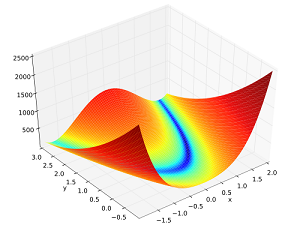
\includegraphics[width=0.75\textwidth]{function_optimization/rosenbrock_function.png}
\caption{The Rosenbrock's function in $2$
variables.}\label{RosenbrockFunction}
\end{center}
\end{figure}

The minimal argument of the Rosenbrock's function is found at
$(1, \ldots, 1)$. The minimum value of that
function is $= 0$. Figure \ref{RosenbrockFunction}
is a plot of the Rosenbrock's function in $2$ variables.

\subsection*{The Rastrigin's function}

The Rastrigin's function is based on the De Jong's function with the
addition of cosine modulation to produce many local minima. As a
result, this function is highly multimodal. However, the location of
the minima are regularly distributed. The Rastrigin's function
optimization problem in $d$ variables can be stated as:


\begin{figure}[h!]
\begin{center}
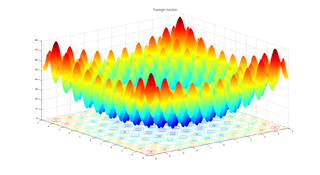
\includegraphics[width=0.75\textwidth]{function_optimization/rastrigin_function.png}
\caption{The Rastrigin's function in $2$
variables.}\label{RastriginFunction}
\end{center}
\end{figure}

The global minimum of the Rastrigin's Function is at $(0,\ldots,0)$. 
At this minimal argument the value of the function is
$0$. Figure \ref{RastriginFunction} is a plot of the
Rastrigin's function in $2$ variables.

The gradient vector for the Rastrigin's function is given by
\noindent and the Hessian matrix by



 
%%%%%%%%%%%%%%%%%%%%%%%%%%%%%%%%%%%%%%%%%%%%%%%%%%%%%%%%%%%%%%%%%%%%%%%%%%%%%%%%%%%%

\appendix

\chapter{Unit testing}\label{UnitTesting}
\section*{The unit testing development pattern}

Unit testing is the process of creating integrated tests into a source code, and running those tests every time it is to be built. In that way, the build process checks not only for syntax errors, but for semantic errors as well. 

In that regard, unit testing is generally considered a development pattern, in which the tests would be written even before the actual code. If tests are written first, they:

\begin{itemize}
\item[-] Describe what the code is supposed to do in concrete, verifiable terms.
\item[-] Provide examples of code use rather than just  academic descriptions. 
\item[-] Provide a way to verify when the code is finished (when all the tests run correctly). 
\end{itemize}

\section*{Related code}

There exist several available frameworks for incorporating test cases in C++ code, such as CppUnit or Cpp test. 
However, for portability reasons, \texttt{OpenNN} comes with a simple unit testing utility class for handing automated tests. 
Also, every classes and methods have test classes and methods associated. 

\subsubsection*{The UnitTesting class in OpenNN}

\texttt{OpenNN} includes the \lstinline"UnitTesting" abstract class to provide some simple mechanisms to build test cases and test suites.

\subsubsection*{Constructor}

Unit testing is to be performed on classes and methods. Therefore the \lstinline"UnitTesting" class is abstract and it can't be instantiated. Concrete test classes must be derived here. 

\subsubsection*{Members}

The \lstinline"UnitTesting" class has the following members:

\begin{itemize}
\item[-] The counted number of tests.
\item[-] The counted number of passed tests.
\item[-] The counted number of failed tests.
\item[-] The output message. 
\end{itemize}

That members can be accessed or modified using get and set methods, respectively. 

\subsubsection*{Methods}

Derived classes must implement the pure virtual \lstinline"run_test_case" method, which includes all testing methods. The use of this method is as follows:

\begin{lstlisting}
TestMockClass tmc;
tmc.run_test_case();
\end{lstlisting}

The \lstinline"assert_true" and \lstinline"assert_false" methods are used to prove if some condition is satisfied or not, respectively. If the result is correct, the counter of passed tests is increased by one; otherwise the counter of failed tests is increased by one, 

\begin{lstlisting}
unsigned int a = 0;
unsigned int b = 0;

TestMockClass tmc;
tmc.assert_true(a == b, "Increase tests passed count");
tmc.assert_false(a == b, "Increase tests failed count");
\end{lstlisting}

Finally, the \lstinline"print_results" method prints the testing outcome,

\begin{lstlisting}
TestMockClass tmc;
tmc.run_test_case();
tmc.print_results();
\end{lstlisting}

\subsubsection*{The unit testing classes}

Every single class in \texttt{OpenNN} has a test class associated, and every single method of that class has also a test method associated. 

On the other hand, a test suite of all the classes distributed within \texttt{OpenNN} can be found in the folder \lstinline"AllTests".


\bibliography{bibliography}\bibliographystyle{plain}

%\printindex

\end{document}
